%----------------------------------------------------------------------------------------
% Preambulo y Configuración
%----------------------------------------------------------------------------------------

\documentclass[
    11pt,
    spanish,
    singlespacing,
    parskip,
    headsepline,
    bookmarks=true,
    unicode=true,
    pdftoolbar=true,
    pdfmenubar=true,
    pdffitwindow=false,
    colorlinks=true,
    linkcolor=blue,
    citecolor=blue,
    urlcolor=blue
]{MastersDoctoralThesis}

\usepackage[utf8]{inputenc} % Codificación de entrada UTF-8
\usepackage[T1]{fontenc}    % Codificación de salida para caracteres especiales
\usepackage{graphicx}       % Manejo de gráficos
\usepackage{eso-pic}        % Permite agregar fondos
\usepackage{hyperref}       % Manejo de hipervínculos y marcadores
\usepackage{tikz}           % Manejo de gráficos
\usepackage{multirow}
\usetikzlibrary{positioning, calc, babel}

% Redefinición de caracteres problemáticos en marcadores
\hypersetup{
    pdftitle={Asignación de características musicales para ambientación comercial},
    pdfauthor={Ing. Carlos Alberto Rivas Araque},
    pdfkeywords={Inteligencia Artificial, Aprendizaje Automático, Procesamiento de Señales, Análisis de Datos, Extracción de información musical},
    pdfstartview={FitH},
    unicode=true,
    colorlinks=true,
    linkcolor=blue,
    citecolor=blue,
    urlcolor=blue
}

\pdfstringdefDisableCommands{%
  \def\texttt#1{#1}%
  \def\textbf#1{#1}%
  \def\textit#1{#1}%
  \def\"{\"}%
  \def\~{~}%
  \def\'{'}%
  \def\^{}%
  \def\textunderscore{\_} % Manejo del subrayado en marcadores
}


% Definir comandos requeridos por la clase
\newcommand{\degreename}{Carrera de Especialización en Inteligencia Artificial} % Cambia según tu título
\newcommand{\univname}{Universidad de Buenos Aires} % Cambia según tu universidad
\newcommand{\keywordnames}{Inteligencia Artificial, Aprendizaje Automático, Análisis de Datos, Extracción de información musical}
%----------------------------------------------------------------------------------------
% Documento Principal
%----------------------------------------------------------------------------------------

\begin{document}

% Configuración de la portada
\posgrado{Carrera de Especialización en Inteligencia Artificial}
\keywords{Inteligencia Artificial, Aprendizaje Automático, Análisis de Datos, Extracción de información musical}

% Incluir la portada desde un archivo separado
\include{portada}

% Configuración del contenido preliminar
\frontmatter % Usar numeración romana para las páginas preliminares
\pagestyle{plain} % Estilo de encabezado simple

%----------------------------------------------------------------------------------------
% Resumen
%----------------------------------------------------------------------------------------

\begin{abstract}
\addchaptertocentry{\abstractname} % Agregar resumen al índice
En la presente memoria se describe el diseño e implementación de un sistema que extrae información de las canciones y las etiqueta automáticamente a partir de su audio. Este trabajo fue desarrollado para la empresa Plusyc Live con el fin de optimizar el armado de catálogos musicales destinados a la ambientación de distintos espacios comerciales.

Para la elaboración de este trabajo fueron fundamentales los conocimientos adquiridos durante la carrera sobre tratamiento de datos estadísticos, modelos de árboles de clasificación y regresión, perceptrones multicapa, aprendizaje por transferencia, y puesta en producción.
\end{abstract}

%----------------------------------------------------------------------------------------
% Agradecimientos
%----------------------------------------------------------------------------------------
%
%%\begin{acknowledgements}
%%\vspace{1.5cm}
%%Esta sección es para agradecimientos personales y es totalmente \textbf{OPCIONAL}.
%%\end{acknowledgements}

%----------------------------------------------------------------------------------------
% Índice
%----------------------------------------------------------------------------------------

\tableofcontents
\listoffigures
\listoftables

%----------------------------------------------------------------------------------------
% Dedicatoria
%----------------------------------------------------------------------------------------

%%\dedicatory{\textbf{Dedicado a... [OPCIONAL]}}

%----------------------------------------------------------------------------------------
% Capítulos
%----------------------------------------------------------------------------------------

\mainmatter % Iniciar numeración numérica para el contenido principal
\pagestyle{thesis} % Estilo de encabezado de tesis

% Incluir capítulos desde archivos separados
% Chapter 1

\chapter{Introducción general} % Main chapter title

\label{Chapter1} % For referencing the chapter elsewhere, use \ref{Chapter1} 
\label{IntroGeneral}

% Tudos os capítulos deben comenzar con un breve párrafo introductorio que indique cuál es el contenido que se encontrará al leerlo.  La redacción sobre el contenido de la memoria debe hacerse en presente y todo lo referido al proyecto en pasado, siempre de modo impersonal.

En este capítulo se introduce la definición de la extracción de información musical, se expone la problemática que motivó la búsqueda de una solución automatizada para la asignación de características musicales a partir del audio de canciones, y se detalla el alcance de la solución propuesta. Finalmente, se realiza una revisión general de las soluciones existentes.
%----------------------------------------------------------------------------------------

% Define some commands to keep the formatting separated from the content 
\newcommand{\keyword}[1]{\textbf{#1}}
\newcommand{\tabhead}[1]{\textbf{#1}}
\newcommand{\code}[1]{\texttt{#1}}
\newcommand{\file}[1]{\texttt{\bfseries#1}}
\newcommand{\option}[1]{\texttt{\itshape#1}}
\newcommand{\grados}{$^{\circ}$}

%----------------------------------------------------------------------------------------

%\section{Introducción}

%----------------------------------------------------------------------------------------
\section{Extracción de información musical}

% Introducción a la extracción de información musical (MIR).

La extracción de información musical, comúnmente conocida como MIR (por su sigla en inglés, \textit{Music Information Retrieval}), procesa, analiza y organiza datos musicales \citep{Downie2003}.

Los sistemas MIR abarcan el procesamiento digital de señales (DSP) y el aprendizaje automático, y permiten automatizar tareas como el etiquetado de canciones, la clasificación de géneros o el reconocimiento de estados de ánimo a partir del audio digital \citep{Casey2008}.

La aplicación de estas tecnologías en el contexto comercial resulta fundamental para la personalización y ambientación de espacios físicos. La literatura académica señala que la música de fondo (\textit{background music}) no es un elemento pasivo, sino un factor ambiental estratégico. Investigaciones en el área muestran que componentes estructurales de la música alteran de forma predecible la excitación emocional (\textit{arousal}), la percepción del tiempo y la intención de compra de los consumidores en entornos minoristas y de servicios \citep{bruner1990music, garlin2006setting, roschk2017calibrating}. 

Para lograr una personalización ambiental efectiva en cada comercio, es necesario seleccionar pistas musicales que se ajusten a criterios sonoros y emocionales específicos dictados por la identidad de cada marca. La curaduría manual resulta inescalable debido a la gran magnitud de los catálogos musicales; en consecuencia, es importante desarrollar un producto que implemente técnicas MIR para caracterizar automáticamente los archivos de audio de las canciones de grandes repositorios de audio, para el uso de las características en sistemas que llevan música a espacios comerciales, según las necesidades específicas de cada lugar.
% Acá tiene un ejemplo de una ``subsubsección'' que es el cuarto nivel de ordenamiento del texto, después de capítulo, sección y subsección.  Como se puede ver, las subsubsecciones no van numeradas en el cuerpo del documento ni en el índice.  El formato está definido por la plantilla y no debe ser modificado.

% \subsection{Guía matemática rápida para \LaTeX{}}

% Si estás escribiendo un documento con mucho contenido matemático, entonces es posible que desees leer el documento de la AMS (American Mathematical Society) llamado, \enquote{A Short Math Guide for \LaTeX{}}. Se puede encontrar en línea en el siguiente link: \url{http://www.ams.org/tex/amslatex.html} en la sección \enquote{Additional Documentation} hacia la parte inferior de la página.


%----------------------------------------------------------------------------------------

\section{Contexto de aplicación}

% MIR en el contexto de la ambientación comercial.
El trabajo se realiza para dar respuesta a una necesidad tecnológica de Plusyc Live SAS \citep{plusyc_web}, una empresa dedicada a la creación de experiencias musicales personalizadas para locales comerciales. La plataforma de la compañía crea listas de reproducción basadas en las características musicales de un catálogo de canciones. 

Anteriormente, la asignación de estas características dependía del consumo de interfaces de programación de aplicaciones (API) de terceros. Esta metodología generaba restricciones de disponibilidad, incrementos en los costos operativos y limitaba la autonomía de la empresa. 

Con la implementación de este trabajo, la empresa cuenta con un sistema de inteligencia artificial que caracteriza automáticamente canciones a partir de su archivo de audio. Esto reduce la dependencia de servicios externos y mejora la escalabilidad y autonomía de la aplicación; de esta manera se fortalece la experiencia musical personalizada que la empresa ofrece a los comercios.

%----------------------------------------------------------------------------------------

\section{Objetivos y alcance}

Esta sección define las metas. Se presenta el objetivo general y los objetivos específicos, y el conjunto de características musicales consideradas.

\subsection{Objetivo general}

Desarrollar un sistema basado en inteligencia artificial para predecir las características musicales de las canciones del catálogo de Plusyc Live a partir de su archivo de audio y reducir la dependencia de servicios de terceros.

\subsection{Objetivos específicos}

Para alcanzar el objetivo general, se definen los siguientes objetivos específicos:

\begin{itemize}
  \item Seleccionar y analizar un conjunto de datos musicales pertinente para el entrenamiento de modelos de aprendizaje supervisado.
  \item Extraer representaciones numéricas y descriptores semánticos a partir de las señales de audio originales.
  \item Ejecutar el análisis exploratorio de datos (EDA) y el preprocesamiento de las variables.
  \item Entrenar modelos de aprendizaje supervisado para la predicción de las características objetivo.
  \item Evaluar el rendimiento de los modelos y seleccionar los de mejor desempeño.
  \item Desplegar los modelos en un entorno productivo para su integración operativa.
\end{itemize}
% Definición de lo que abarca el trabajo y lo que no se compromete.

% El trabajo incluye la asignación de las características musicales definidas en la tabla~\ref{tab:caracteristicas_ia}.
% Las definiciones de las características agrupadas como básicas y perceptibles tienen como origen la documentación de Spotify~\cite{spotify}.

% \begin{table}[htpb]
%   \centering
%   \caption[Características predictivas]{Definición, ejemplos y tipo de problema de aprendizaje supervisado por característica.}
%   \label{tab:caracteristicas_ia}
%   \renewcommand{\arraystretch}{1.2}
%   \begin{tabular}{@{}l p{5.5cm} p{3.5cm} l@{}}
%     \toprule
%     \textbf{Característica} & \textbf{Definición} & \textbf{Ejemplos} & \textbf{Tipo de problema} \\
%     \midrule
%     \multicolumn{4}{@{}l}{\textbf{Básicas}} \\
%     \midrule
%     \textit{Key} & Tonalidad estimada de la pista mapeada a números enteros (\textit{Pitch Class}). & 0 (Do), 1 (Do\#), 2 (Re) & Clasificación \\
%     \textit{Mode} & Modalidad (mayor o menor) del contenido melódico. & 1 (Mayor), 0 (Menor) & Clasificación \\
%     \textit{Tempo} & Tempo global estimado en pulsaciones por minuto (BPM). & 120 BPM, 85 BPM & Regresión \\
%     \textit{Loudness} & Volumen global promedio en decibeles (dB). & -5.2 dB, -12.4 dB & Regresión \\
%     \midrule
%     \multicolumn{4}{@{}l}{\textbf{Perceptibles}} \\
%     \midrule
%     \textit{Acousticness} & Confianza de que la pista es acústica (0.0 a 1.0). & 0.95, 0.10 & Regresión \\
%     \textit{Danceability} & Capacidad de ser bailable según tempo y ritmo (0.0 a 1.0). & 0.85, 0.20 & Regresión \\
%     \textit{Energy} & Medida de intensidad y actividad (0.0 a 1.0). & 0.90 & Regresión \\
%     \textit{Instrumentalness} & Probabilidad de ausencia de contenido vocal (0.0 a 1.0). & 0.90 (sin voz), 0.05 (cantada) & Regresión \\
%     \textit{Liveness} & Confianza de grabación con público en vivo (0.0 a 1.0). & 0.85 (concierto), 0.10 (estudio) & Regresión \\
%     \textit{Speechiness} & Presencia de palabras habladas (0.0 a 1.0). & 0.85 (conversación), 0.5 (rap), 0.05 (música) & Regresión \\
%     \textit{Valence} & Positividad musical transmitida (0.0 a 1.0). & 0.90, 0.15 & Regresión \\
%     \midrule
%     \multicolumn{4}{@{}l}{\textbf{Clasificables por ánimo y género}} \\
%     \midrule
%     \textit{Primary Mood} & Estado de ánimo o emoción predominante. & \textit{Energizing, Lively, Empowering} & Clasificación \\
%     \textit{Secondary Mood} & Estados de ánimo complementarios. & \textit{Euphoric Energy, Energetic Anxious} & Clasificación \\
%     \textit{Suggested Genres} & Género musical sugerido. & \textit{Chill House, EDM} & Clasificación \\
%     \bottomrule
%   \end{tabular}
% \end{table}

\subsection{Alcance}

El alcance de este trabajo comprende la predicción computacional de trece características musicales, que se agrupan en tres categorías principales:

\begin{itemize}
    \item Básicas: tonalidad (key), modo (mode), tempo y volumen (loudness).
    \item Perceptibles: nivel acústico (acousticness), bailabilidad (danceability), energía (energy), instrumentalidad (instrumentalness), presencia de público (liveness), presencia de voz (speechiness) y positividad (valence).
    \item Clasificables por ánimo y género: estados de ánimo predominantes (primary moods), estados de ánimo secundarios (secondary moods) y géneros sugeridos (suggested genres).
\end{itemize}

Para cada una de las características mencionadas se busca cumplir con los objetivos específicos definidos.

% El presente trabajo no incluye:

% \begin{itemize}
%   \item Asignación del subconjunto de otras características que no requieren de inteligencia artificial para su asignación.
%   \item Análisis de las letras de las canciones.
%   \item Desarrollo de interfaces gráficas de usuario.
%   \item Mantenimiento y monitoreo a largo plazo.
% \end{itemize}

%----------------------------------------------------------------------------------------

\section{Estado del arte}

% Soluciones en la industria.

En el campo de la extracción de información musical existen diversas herramientas computacionales para el análisis de audio. Por un lado, se encuentran las bibliotecas de procesamiento digital de señales, que permiten extraer representaciones numéricas a partir de archivos de audio. Además, existen modelos preentrenados capaces de obtener información semántica y servicios comerciales orientados a inferir etiquetas de alto nivel.

\subsection{Procesamiento digital de señales y extracción a bajo nivel}

Existen bibliotecas de software para extraer descriptores numéricos de bajo nivel, como Librosa \citep{librosa} y Essentia \citep{essentia}. 

Las bibliotecas de procesamiento digital de señales proveen funciones para representar la señal digital en arreglos numéricos, como espectrogramas y cromagramas. Este tipo de transformaciones matemáticas son útiles para reducir la dimensionalidad de los archivos de audio y generar variables predictivas para modelos de aprendizaje automático.

\subsection{Modelos preentrenados y soluciones comerciales}

Para la predicción de características semánticas existen modelos de código abierto basados en aprendizaje profundo. Dos ejemplos son la arquitectura musicnn \citep{musicnn} y los modelos entrenados sobre el conjunto de datos AudioSet \citep{audioset}. Estos sistemas clasifican etiquetas musicales generales. Su limitación principal radica en el uso de taxonomías fijas orientadas a los datos con los que fueron entrenados originalmente.
La biblioteca Essentia también incorpora modelos preentrenados para inferir atributos semánticos, y por lo tanto se incluye en esta categoría.

Por su parte, soluciones comerciales como Spotify \citep{spotify} y Gracenote \citep{gracenote} operan en la modalidad de software como servicio (SaaS) y entregan predicciones mediante su interfaz de programación de aplicaciones (API). La gran desventaja es que introducen costos operativos recurrentes y generan dependencia tecnológica hacia el proveedor.

También existen plataformas web que permiten consultar esta información de manera individual. Un ejemplo es Tunebat \citep{Tunebat}, que permite visualizar un conjunto de características, pero restringe la consulta a una canción a la vez. En la figura~\ref{fig:tunebat_screenshot} se presenta un ejemplo de perfil de características musicales de una canción en la plataforma web Tunebat.
En la interfaz se exponen algunas características, como la tonalidad (Si menor o \textit{B Minor}), el \textit{tempo} (153 BPM) y la duración. Asimismo, la herramienta cuantifica algunas características en una escala porcentual de 0 a 100, mostrando para este caso específico niveles de acusticidad (77\%) e instrumentalidad (76\%), una baja probabilidad de presencia de habla (\textit{speechiness} en 4\%) y público en vivo (\textit{liveness} en 9\%), además de registrar el volumen medio en decibelios (-8 dB).

\begin{figure}[htpb]
    \centering
    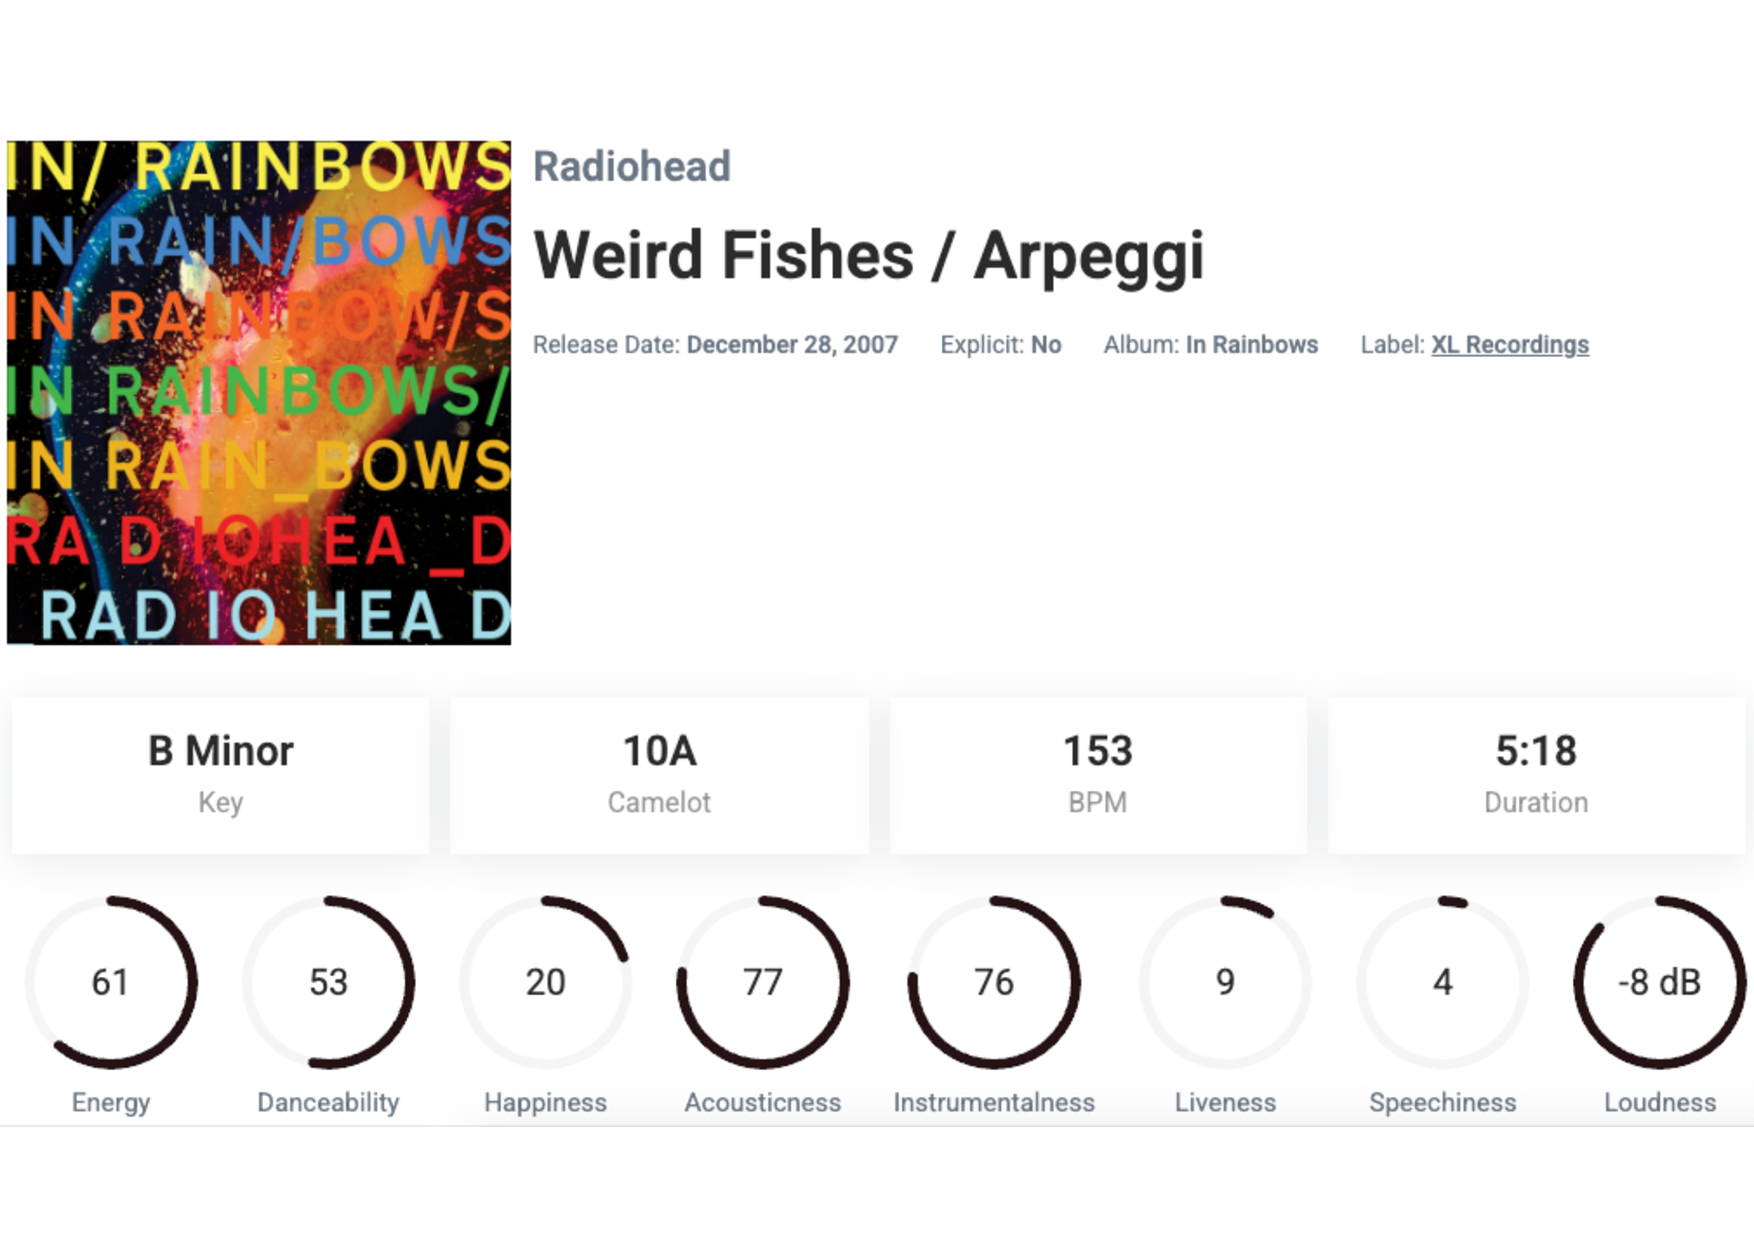
\includegraphics[width=1\textwidth]{Figures/weirdfishes.pdf}
    \caption[Interfaz de consulta en Tunebat]{Ejemplo de visualización de características musicales en Tunebat\protect\footnotemark.}
    \label{fig:tunebat_screenshot}
\end{figure}
\footnotetext{Imagen tomada de \url{https://bit.ly/4nJ8RWg}}
% \subsection{Carpetas}

\subsection{Síntesis comparativa}
\label{subsec:sintesis_estado_arte}

Las tecnologías existentes ofrecen herramientas útiles para el objetivo del trabajo. Las bibliotecas de procesamiento digital de señales permiten extraer representaciones numéricas de las ondas sonoras, y los modelos preentrenados ofrecen representaciones semánticas. Por otro lado, las soluciones comerciales proveen servicios de etiquetado para canciones.
 
Sin embargo, persisten limitaciones operativas para su aplicación directa en el entorno de la empresa. Los servicios de terceros generan costos recurrentes, limitan la cantidad de consultas y crean dependencia tecnológica. Las plataformas web de uso manual no son viables para procesar catálogos con miles de canciones. Además, los modelos no coinciden con las características y las clases específicas que usa Plusyc Live.

Por estos motivos, resulta necesario desarrollar una solución propia. El propósito de este trabajo es aprovechar las técnicas actuales de inteligencia artificial para crear un sistema independiente. Esto permite analizar directamente los archivos de audio, etiquetarlos según las necesidades de la empresa y así reducir la dependencia de proveedores externos.



% Esta plantilla se distribuye como una único archivo .zip que se puede descomprimir en varios archivos y carpetas. Asimismo, se puede consultar el repositorio git para obtener la última versión de los archivos, \url{https://github.com/patriciobos/Plantilla-CESE.git}. Los nombres de las carpetas son, o pretender ser, auto-explicativos.

% \keyword{Appendices} -- Esta es la carpeta donde se deben poner los apéndices. Cada apéndice debe ir en su propio archivo \file{.tex}. Se incluye un ejemplo y una plantilla en la carpeta.

% \keyword{Chapters} -- Esta es la carpeta donde se deben poner los capítulos de la memoria. Cada capítulo debe ir un su propio archivo \file{.tex} por separado.  Se ofrece por defecto, la siguiente estructura de capítulos y se recomienda su utilización dentro de lo posible:

% \begin{itemize}
% \item Capítulo 1: Introducción general	
% \item Capítulo 2: Introducción específica
% \item Capítulo 3: Diseño e implementación
% \item Capítulo 4: Ensayos y resultados
% \item Capítulo 5: Conclusiones

% \end{itemize}

% Esta estructura de capítulos es la que se recomienda para las memorias de la especialización.

% \keyword{Figures} -- Esta carpeta contiene todas las figuras de la memoria.  Estas son las versiones finales de las imágenes que van a ser incluidas en la memoria.  Pueden ser imágenes en formato \textit{raster}\footnote{\url{https://en.wikipedia.org/wiki/Raster_graphics}} como \file{.png}, \file{.jpg} o en formato vectoriales\footnote{\url{https://en.wikipedia.org/wiki/Vector_graphics}} como \file{.pdf}, \file{.ps}.  Se debe notar que utilizar imágenes vectoriales disminuye notablemente el peso del documento final y acelera el tiempo de compilación por lo que es recomendable su utilización siempre que sea posible.

% \subsection{Archivos}

% También están incluidos varios archivos, la mayoría de ellos son de texto plano y se puede ver su contenido en un editor de texto. Después de la compilación inicial, se verá que más archivos auxiliares son creados por \ LaTeX{} o BibTeX, pero son de uso interno y no es necesario hacer nada en particular con ellos.  Toda la información necesaria para compilar el documento se encuentra en los archivos \file{.tex}, \file{.bib}, \file{.cls} y en las imágenes de la carpeta Figures.

% \keyword{referencias.bib} - este es un archivo importante que contiene toda la información de referencias bibliográficas que se utilizarán para las citas en la memoria en conjunto con BibTeX. Usted puede escribir las entradas bibliográficas en forma manual, aunque existen también programas de gestión de referencias que facilitan la creación y gestión de las referencias y permiten exportarlas en formato BibTeX.  También hay disponibles sitios web como \url{books.google.com} que permiten obtener toda la información necesaria para una cita en formato BibTeX. Ver sección \ref{sec:biblio}

% \keyword{MastersDoctoralThesis.cls} -- este es un archivo importante. Es el archivos con la clase que le informa a \LaTeX{} cómo debe dar formato a la memoria. El usuario de la plantilla no debería necesitar modificar nada de este archivo.

% \keyword{memoria.pdf} -- esta es su memoria con una tipografía bellamente compuesta (en formato de archivo PDF) creado por \LaTeX{}. Se distribuye con la plantilla y después de compilar por primera vez sin hacer ningún cambio se debería obtener una versión idéntica a este documento.

% \keyword{memoria.tex} -- este es un archivo importante. Este es el archivo que tiene que compilar \LaTeX{} para producir la memoria como un archivo PDF. Contiene un marco de trabajo y estructuras que le indican a \LaTeX{} cómo diagramar la memoria.  Está altamente comentado para que se pueda entender qué es lo que realiza cada línea de código y por qué está incluida en ese lugar.  En este archivo se debe completar la información personalizada de las primeras sección según se indica en la sección \ref{sec:FillingFile}.

% Archivos que \emph{no} forman parte de la distribución de la plantilla pero que son generados por \LaTeX{} como archivos auxiliares necesarios para la producción de la memoria.pdf son:

% \keyword{memoria.aux} -- este es un archivo auxiliar generado por \LaTeX{}, si se borra \LaTeX{} simplemente lo regenera cuando se compila el archivo principal \file{memoria.tex}.

% \keyword{memoria.bbl} -- este es un archivo auxiliar generado por BibTeX, si se borra BibTeX simplemente lo regenera cuando se compila el archivo principal \file{memoria.tex}. Mientras que el archivo \file{.bib} contiene todas las referencias que hay, este archivo \file{.bbl} contine sólo las referencias que han sido citadas y se utiliza para la construcción de la bibiografía.

% \keyword{memoria.blg} -- este es un archivo auxiliar generado por BibTeX, si se borra BibTeX simplemente lo regenera cuando se compila el archivo principal \file{memoria.tex}.

% \keyword{memoria.lof} -- este es un archivo auxiliar generado por \LaTeX{}, si se borra \LaTeX{} simplemente lo regenera cuando se compila el archivo principal \file{memoria.tex}.  Le indica a \LaTeX{} cómo construir la sección \emph{Lista de Figuras}.
 
% \keyword{memoria.log} --  este es un archivo auxiliar generado por \LaTeX{}, si se borra \LaTeX{} simplemente lo regenera cuando se compila el archivo principal \file{memoria.tex}. Contiene mensajes de \LaTeX{}. Si se reciben errores o advertencias durante la compilación, se guardan en este archivo \file{.log}.

% \keyword{memoria.lot} -- este es un archivo auxiliar generado por \LaTeX{}, si se borra \LaTeX{} simplemente lo regenera cuando se compila el archivo principal \file{memoria.tex}.  Le indica a \LaTeX{} cómo construir la sección \emph{Lista de Tablas}.

% \keyword{memoria.out} -- este es un archivo auxiliar generado por \LaTeX{}, si se borra \LaTeX{} simplemente lo regenera cuando se compila el archivo principal \file{memoria.tex}.

% De esta larga lista de archivos, sólo aquellos con la extensión \file{.bib}, \file{.cls} y \file{.tex} son importantes.  Los otros archivos auxiliares pueden ser ignorados o borrados ya que \LaTeX{} y BibTeX los regenerarán durante la compilación.

%----------------------------------------------------------------------------------------


% \subsection{Paquetes adicionales}

% Si bien durante el proceso de instalación de TexMaker, o cualquier otro editor que se haya elegido, se instalarán en el sistema los paquetes básicos necesarios para trabajar con \LaTeX{}, la plantilla de los trabajos de Especialización y Maestría requieren de paquete adicionales.

% Se indican a continuación los comandos que se deben introducir en la consola de Ubuntu (ctrl + alt + t) para instalarlos:

% \begin{lstlisting}[language=bash]
%   $ sudo apt install texlive-lang-spanish texlive-science 
%   $ sudo apt install texlive-bibtex-extra biber
%   $ sudo apt install texlive texlive-fonts-recommended
%   $ sudo apt install texlive-latex-extra
% \end{lstlisting}


% \subsection{Configurando TexMaker}
% \label{subsec:configurando}



% Una vez instalado el programa y los paquetes adicionales se debe abrir el archivo memoria.tex con el editor para ver una pantalla similar a la que se puede apreciar en la figura \ref{fig:texmaker}. 
% Una vez instalado el programa y los paquetes adicionales se debe abrir el archivo memoria.tex con el editor para ver una pantalla similar a la que se puede apreciar en la figura \ref{fig:texmaker}. 
% Una vez instalado el programa y los paquetes adicionales se debe abrir el archivo memoria.tex con el editor para ver una pantalla similar a la que se puede apreciar en la figura \ref{fig:texmaker}. 
% Una vez instalado el programa y los paquetes adicionales se debe abrir el archivo memoria.tex con el editor para ver una pantalla similar a la que se puede apreciar en la figura \ref{fig:texmaker}. 

% \vspace{1cm}

% \begin{figure}[htbp]
% 	\centering
% 	\includegraphics[width=.5\textwidth]{./Figures/texmaker.png}
% 	\caption{Entorno de trabajo de texMaker.}
% 	\label{fig:texmaker}
% \end{figure}

% \vspace{1cm}

% Notar que existe una vista llamada Estructura a la izquierda de la interfaz que nos permite abrir desde dentro del programa los archivos individuales de los capítulos.  A la derecha se encuentra una vista con el archivo propiamente dicho para su edición. Hacia la parte inferior se encuentra una vista del log con información de los resultados de la compilación.  En esta última vista pueden aparecen advertencias o \textit{warning}, que normalmente pueden ser ignorados, y los errores que se indican en color rojo y deben resolverse para que se genere el PDF de salida.

% Recordar que el archivo que se debe compilar con PDFLaTeX es \file{memoria.tex}, si se tratara de compilar alguno de los capítulos saldría un error.  Para salvar la molestia de tener que cambiar de archivo para compilar cada vez que se realice una modificación en un capítulo, se puede definir el archivo \file{memoria.tex} como ``documento maestro'' yendo al menú opciones -> ``definir documento actual como documento maestro'', lo que permite compilar con PDFLaTeX memoria.tex directamente desde cualquier archivo que se esté modificando . Se muestra esta opción en la figura \ref{fig:docMaestro}.

% \begin{figure}[h]
% 	\centering
% 	\includegraphics[width=\textwidth]{./Figures/docMaestro.png}
% 	\caption{Definir memoria.tex como documento maestro.}
% 	\label{fig:docMaestro}
% \end{figure}

% En el menú herramientas se encuentran las opciones de compilación.  Para producir un archivo PDF a partir de un archivo .tex se debe ejecutar PDFLaTeX (el shortcut es F6). Para incorporar nueva bibliografía se debe utilizar la opción BibTeX del mismo menú herramientas (el shortcut es F11).

% Notar que para actualizar las tablas de contenidos se debe ejecutar PDFLaTeX dos veces.  Esto se debe a que es necesario actualizar algunos archivos auxiliares antes de obtener el resultado final.  En forma similar, para actualizar las referencias bibliográficas se debe ejecutar primero PDFLaTeX, después BibTeX y finalmente PDFLaTeX dos veces por idénticos motivos.

% \section{Personalizando la plantilla, el archivo \file{memoria.tex}}
% \label{sec:FillingFile}

% Para personalizar la plantilla se debe incorporar la información propia en los distintos archivos \file{.tex}. 

% Primero abrir \file{memoria.tex} con TexMaker (o el editor de su preferencia). Se debe ubicar dentro del archivo el bloque de código titulado \emph{INFORMACIÓN DE LA PORTADA} donde se deben incorporar los primeros datos personales con los que se construirá automáticamente la portada.


%----------------------------------------------------------------------------------------

% \section{El código del archivo \file{memoria.tex} explicado}

% El archivo \file{memoria.tex} contiene la estructura del documento y es el archivo de mayor jerarquía de la memoria.  Podría ser equiparable a la función \emph{main()} de un programa en C, o mejor dicho al archivo fuente .c donde se encuentra definida la función main().

% La estructura básica de cualquier documento de \LaTeX{} comienza con la definición de clase del documento, es seguida por un preámbulo donde se pueden agregar funcionalidades con el uso de \texttt{paquetes} (equiparables a bibliotecas de C), y finalmente, termina con el cuerpo del documento, donde irá el contenido de la memoria.

% \lstset{%
%   basicstyle=\small\ttfamily,
%   language=[LaTeX]{TeX}
% }

% \begin{lstlisting}
% \documentclass{article}  <- Definicion de clase
% \usepackage{listings}	 <- Preambulo

% \begin{document}	 <- Comienzo del contenido propio 
% 	Hello world!
% \end{document}
% \end{lstlisting}


% El archivo \file{memoria.tex} se encuentra densamente comentado para explicar qué páginas, secciones y elementos de formato está creando el código \LaTeX{} en cada línea. El código está dividido en bloques con nombres en mayúsculas para que resulte evidente qué es lo que hace esa porción de código en particular. Inicialmente puede parecer que hay mucho código \LaTeX{}, pero es principalmente código para dar formato a la memoria por lo que no requiere intervención del usuario de la plantilla.  Sí se deben personalizar con su información los bloques indicados como:

% \begin{itemize}
% 	\item Informacion de la memoria
% 	\item Resumen
% 	\item Agradecimientos
% 	\item Dedicatoria
% \end{itemize}

% El índice de contenidos, las listas de figura de tablas se generan en forma automática y no requieren intervención ni edición manual por parte del usuario de la plantilla. 

% En la parte final del documento se encuentran los capítulos y los apéndices.  Por defecto se incluyen los 5 capítulos propuestos que se encuentran en la carpeta /Chapters. Cada capítulo se debe escribir en un archivo .tex separado y se debe poner en la carpeta \emph{Chapters} con el nombre \file{Chapter1}, \file{Chapter2}, etc\ldots El código para incluir capítulos desde archivos externos se muestra a continuación.

% \begin{verbatim}
% 	% Chapter 1

\chapter{Introducción general} % Main chapter title

\label{Chapter1} % For referencing the chapter elsewhere, use \ref{Chapter1} 
\label{IntroGeneral}

% Tudos os capítulos deben comenzar con un breve párrafo introductorio que indique cuál es el contenido que se encontrará al leerlo.  La redacción sobre el contenido de la memoria debe hacerse en presente y todo lo referido al proyecto en pasado, siempre de modo impersonal.

En este capítulo se introduce la definición de la extracción de información musical, se expone la problemática que motivó la búsqueda de una solución automatizada para la asignación de características musicales a partir del audio de canciones, y se detalla el alcance de la solución propuesta. Finalmente, se realiza una revisión general de las soluciones existentes.
%----------------------------------------------------------------------------------------

% Define some commands to keep the formatting separated from the content 
\newcommand{\keyword}[1]{\textbf{#1}}
\newcommand{\tabhead}[1]{\textbf{#1}}
\newcommand{\code}[1]{\texttt{#1}}
\newcommand{\file}[1]{\texttt{\bfseries#1}}
\newcommand{\option}[1]{\texttt{\itshape#1}}
\newcommand{\grados}{$^{\circ}$}

%----------------------------------------------------------------------------------------

%\section{Introducción}

%----------------------------------------------------------------------------------------
\section{Extracción de información musical}

% Introducción a la extracción de información musical (MIR).

La extracción de información musical, comúnmente conocida como MIR (por su sigla en inglés, \textit{Music Information Retrieval}), procesa, analiza y organiza datos musicales \citep{Downie2003}.

Los sistemas MIR abarcan el procesamiento digital de señales (DSP) y el aprendizaje automático, y permiten automatizar tareas como el etiquetado de canciones, la clasificación de géneros o el reconocimiento de estados de ánimo a partir del audio digital \citep{Casey2008}.

La aplicación de estas tecnologías en el contexto comercial resulta fundamental para la personalización y ambientación de espacios físicos. La literatura académica señala que la música de fondo (\textit{background music}) no es un elemento pasivo, sino un factor ambiental estratégico. Investigaciones en el área muestran que componentes estructurales de la música alteran de forma predecible la excitación emocional (\textit{arousal}), la percepción del tiempo y la intención de compra de los consumidores en entornos minoristas y de servicios \citep{bruner1990music, garlin2006setting, roschk2017calibrating}. 

Para lograr una personalización ambiental efectiva en cada comercio, es necesario seleccionar pistas musicales que se ajusten a criterios sonoros y emocionales específicos dictados por la identidad de cada marca. La curaduría manual resulta inescalable debido a la gran magnitud de los catálogos musicales; en consecuencia, es importante desarrollar un producto que implemente técnicas MIR para caracterizar automáticamente los archivos de audio de las canciones de grandes repositorios de audio, para el uso de las características en sistemas que llevan música a espacios comerciales, según las necesidades específicas de cada lugar.
% Acá tiene un ejemplo de una ``subsubsección'' que es el cuarto nivel de ordenamiento del texto, después de capítulo, sección y subsección.  Como se puede ver, las subsubsecciones no van numeradas en el cuerpo del documento ni en el índice.  El formato está definido por la plantilla y no debe ser modificado.

% \subsection{Guía matemática rápida para \LaTeX{}}

% Si estás escribiendo un documento con mucho contenido matemático, entonces es posible que desees leer el documento de la AMS (American Mathematical Society) llamado, \enquote{A Short Math Guide for \LaTeX{}}. Se puede encontrar en línea en el siguiente link: \url{http://www.ams.org/tex/amslatex.html} en la sección \enquote{Additional Documentation} hacia la parte inferior de la página.


%----------------------------------------------------------------------------------------

\section{Contexto de aplicación}

% MIR en el contexto de la ambientación comercial.
El trabajo se realiza para dar respuesta a una necesidad tecnológica de Plusyc Live SAS \citep{plusyc_web}, una empresa dedicada a la creación de experiencias musicales personalizadas para locales comerciales. La plataforma de la compañía crea listas de reproducción basadas en las características musicales de un catálogo de canciones. 

Anteriormente, la asignación de estas características dependía del consumo de interfaces de programación de aplicaciones (API) de terceros. Esta metodología generaba restricciones de disponibilidad, incrementos en los costos operativos y limitaba la autonomía de la empresa. 

Con la implementación de este trabajo, la empresa cuenta con un sistema de inteligencia artificial que caracteriza automáticamente canciones a partir de su archivo de audio. Esto reduce la dependencia de servicios externos y mejora la escalabilidad y autonomía de la aplicación; de esta manera se fortalece la experiencia musical personalizada que la empresa ofrece a los comercios.

%----------------------------------------------------------------------------------------

\section{Objetivos y alcance}

Esta sección define las metas. Se presenta el objetivo general y los objetivos específicos, y el conjunto de características musicales consideradas.

\subsection{Objetivo general}

Desarrollar un sistema basado en inteligencia artificial para predecir las características musicales de las canciones del catálogo de Plusyc Live a partir de su archivo de audio y reducir la dependencia de servicios de terceros.

\subsection{Objetivos específicos}

Para alcanzar el objetivo general, se definen los siguientes objetivos específicos:

\begin{itemize}
  \item Seleccionar y analizar un conjunto de datos musicales pertinente para el entrenamiento de modelos de aprendizaje supervisado.
  \item Extraer representaciones numéricas y descriptores semánticos a partir de las señales de audio originales.
  \item Ejecutar el análisis exploratorio de datos (EDA) y el preprocesamiento de las variables.
  \item Entrenar modelos de aprendizaje supervisado para la predicción de las características objetivo.
  \item Evaluar el rendimiento de los modelos y seleccionar los de mejor desempeño.
  \item Desplegar los modelos en un entorno productivo para su integración operativa.
\end{itemize}
% Definición de lo que abarca el trabajo y lo que no se compromete.

% El trabajo incluye la asignación de las características musicales definidas en la tabla~\ref{tab:caracteristicas_ia}.
% Las definiciones de las características agrupadas como básicas y perceptibles tienen como origen la documentación de Spotify~\cite{spotify}.

% \begin{table}[htpb]
%   \centering
%   \caption[Características predictivas]{Definición, ejemplos y tipo de problema de aprendizaje supervisado por característica.}
%   \label{tab:caracteristicas_ia}
%   \renewcommand{\arraystretch}{1.2}
%   \begin{tabular}{@{}l p{5.5cm} p{3.5cm} l@{}}
%     \toprule
%     \textbf{Característica} & \textbf{Definición} & \textbf{Ejemplos} & \textbf{Tipo de problema} \\
%     \midrule
%     \multicolumn{4}{@{}l}{\textbf{Básicas}} \\
%     \midrule
%     \textit{Key} & Tonalidad estimada de la pista mapeada a números enteros (\textit{Pitch Class}). & 0 (Do), 1 (Do\#), 2 (Re) & Clasificación \\
%     \textit{Mode} & Modalidad (mayor o menor) del contenido melódico. & 1 (Mayor), 0 (Menor) & Clasificación \\
%     \textit{Tempo} & Tempo global estimado en pulsaciones por minuto (BPM). & 120 BPM, 85 BPM & Regresión \\
%     \textit{Loudness} & Volumen global promedio en decibeles (dB). & -5.2 dB, -12.4 dB & Regresión \\
%     \midrule
%     \multicolumn{4}{@{}l}{\textbf{Perceptibles}} \\
%     \midrule
%     \textit{Acousticness} & Confianza de que la pista es acústica (0.0 a 1.0). & 0.95, 0.10 & Regresión \\
%     \textit{Danceability} & Capacidad de ser bailable según tempo y ritmo (0.0 a 1.0). & 0.85, 0.20 & Regresión \\
%     \textit{Energy} & Medida de intensidad y actividad (0.0 a 1.0). & 0.90 & Regresión \\
%     \textit{Instrumentalness} & Probabilidad de ausencia de contenido vocal (0.0 a 1.0). & 0.90 (sin voz), 0.05 (cantada) & Regresión \\
%     \textit{Liveness} & Confianza de grabación con público en vivo (0.0 a 1.0). & 0.85 (concierto), 0.10 (estudio) & Regresión \\
%     \textit{Speechiness} & Presencia de palabras habladas (0.0 a 1.0). & 0.85 (conversación), 0.5 (rap), 0.05 (música) & Regresión \\
%     \textit{Valence} & Positividad musical transmitida (0.0 a 1.0). & 0.90, 0.15 & Regresión \\
%     \midrule
%     \multicolumn{4}{@{}l}{\textbf{Clasificables por ánimo y género}} \\
%     \midrule
%     \textit{Primary Mood} & Estado de ánimo o emoción predominante. & \textit{Energizing, Lively, Empowering} & Clasificación \\
%     \textit{Secondary Mood} & Estados de ánimo complementarios. & \textit{Euphoric Energy, Energetic Anxious} & Clasificación \\
%     \textit{Suggested Genres} & Género musical sugerido. & \textit{Chill House, EDM} & Clasificación \\
%     \bottomrule
%   \end{tabular}
% \end{table}

\subsection{Alcance}

El alcance de este trabajo comprende la predicción computacional de trece características musicales, que se agrupan en tres categorías principales:

\begin{itemize}
    \item Básicas: tonalidad (key), modo (mode), tempo y volumen (loudness).
    \item Perceptibles: nivel acústico (acousticness), bailabilidad (danceability), energía (energy), instrumentalidad (instrumentalness), presencia de público (liveness), presencia de voz (speechiness) y positividad (valence).
    \item Clasificables por ánimo y género: estados de ánimo predominantes (primary moods), estados de ánimo secundarios (secondary moods) y géneros sugeridos (suggested genres).
\end{itemize}

Para cada una de las características mencionadas se busca cumplir con los objetivos específicos definidos.

% El presente trabajo no incluye:

% \begin{itemize}
%   \item Asignación del subconjunto de otras características que no requieren de inteligencia artificial para su asignación.
%   \item Análisis de las letras de las canciones.
%   \item Desarrollo de interfaces gráficas de usuario.
%   \item Mantenimiento y monitoreo a largo plazo.
% \end{itemize}

%----------------------------------------------------------------------------------------

\section{Estado del arte}

% Soluciones en la industria.

En el campo de la extracción de información musical existen diversas herramientas computacionales para el análisis de audio. Por un lado, se encuentran las bibliotecas de procesamiento digital de señales, que permiten extraer representaciones numéricas a partir de archivos de audio. Además, existen modelos preentrenados capaces de obtener información semántica y servicios comerciales orientados a inferir etiquetas de alto nivel.

\subsection{Procesamiento digital de señales y extracción a bajo nivel}

Existen bibliotecas de software para extraer descriptores numéricos de bajo nivel, como Librosa \citep{librosa} y Essentia \citep{essentia}. 

Las bibliotecas de procesamiento digital de señales proveen funciones para representar la señal digital en arreglos numéricos, como espectrogramas y cromagramas. Este tipo de transformaciones matemáticas son útiles para reducir la dimensionalidad de los archivos de audio y generar variables predictivas para modelos de aprendizaje automático.

\subsection{Modelos preentrenados y soluciones comerciales}

Para la predicción de características semánticas existen modelos de código abierto basados en aprendizaje profundo. Dos ejemplos son la arquitectura musicnn \citep{musicnn} y los modelos entrenados sobre el conjunto de datos AudioSet \citep{audioset}. Estos sistemas clasifican etiquetas musicales generales. Su limitación principal radica en el uso de taxonomías fijas orientadas a los datos con los que fueron entrenados originalmente.
La biblioteca Essentia también incorpora modelos preentrenados para inferir atributos semánticos, y por lo tanto se incluye en esta categoría.

Por su parte, soluciones comerciales como Spotify \citep{spotify} y Gracenote \citep{gracenote} operan en la modalidad de software como servicio (SaaS) y entregan predicciones mediante su interfaz de programación de aplicaciones (API). La gran desventaja es que introducen costos operativos recurrentes y generan dependencia tecnológica hacia el proveedor.

También existen plataformas web que permiten consultar esta información de manera individual. Un ejemplo es Tunebat \citep{Tunebat}, que permite visualizar un conjunto de características, pero restringe la consulta a una canción a la vez. En la figura~\ref{fig:tunebat_screenshot} se presenta un ejemplo de perfil de características musicales de una canción en la plataforma web Tunebat.
En la interfaz se exponen algunas características, como la tonalidad (Si menor o \textit{B Minor}), el \textit{tempo} (153 BPM) y la duración. Asimismo, la herramienta cuantifica algunas características en una escala porcentual de 0 a 100, mostrando para este caso específico niveles de acusticidad (77\%) e instrumentalidad (76\%), una baja probabilidad de presencia de habla (\textit{speechiness} en 4\%) y público en vivo (\textit{liveness} en 9\%), además de registrar el volumen medio en decibelios (-8 dB).

\begin{figure}[htpb]
    \centering
    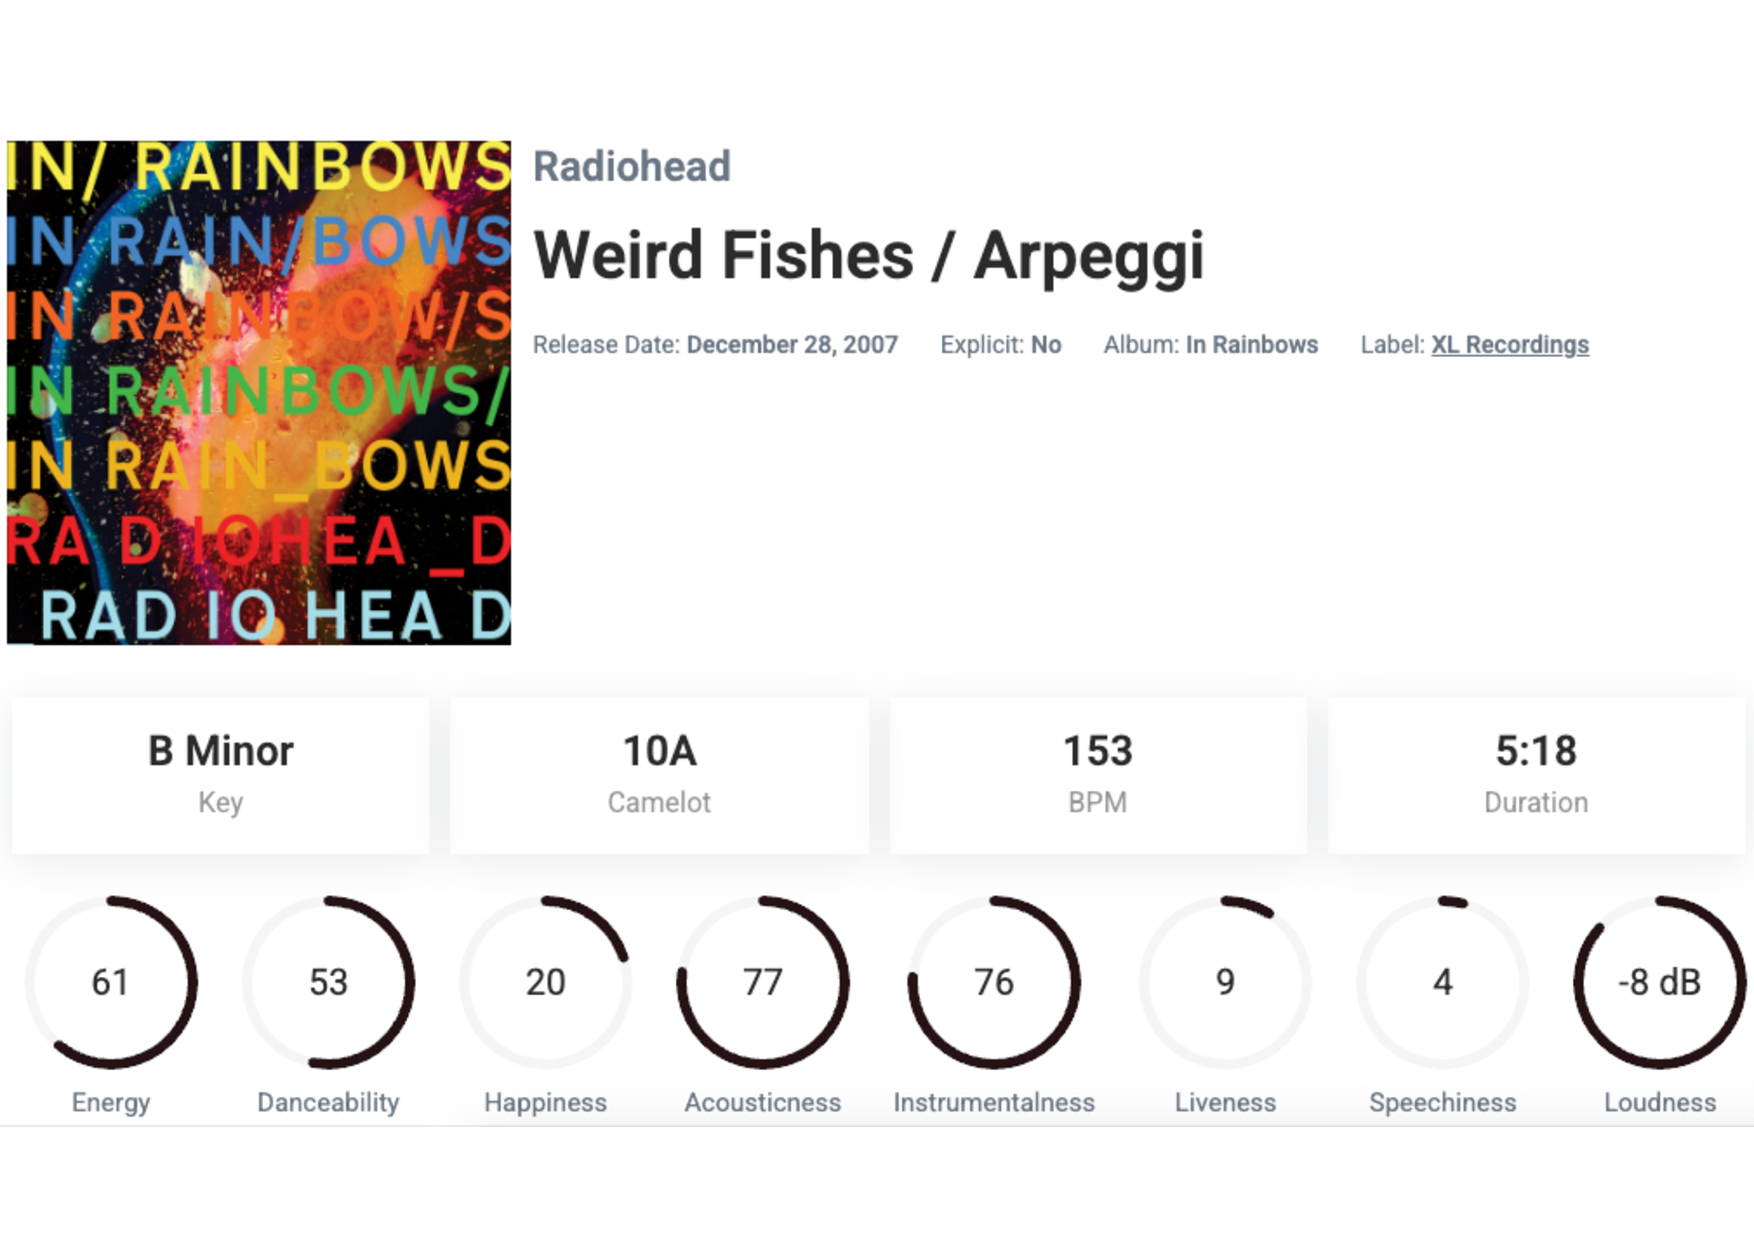
\includegraphics[width=1\textwidth]{Figures/weirdfishes.pdf}
    \caption[Interfaz de consulta en Tunebat]{Ejemplo de visualización de características musicales en Tunebat\protect\footnotemark.}
    \label{fig:tunebat_screenshot}
\end{figure}
\footnotetext{Imagen tomada de \url{https://bit.ly/4nJ8RWg}}
% \subsection{Carpetas}

\subsection{Síntesis comparativa}
\label{subsec:sintesis_estado_arte}

Las tecnologías existentes ofrecen herramientas útiles para el objetivo del trabajo. Las bibliotecas de procesamiento digital de señales permiten extraer representaciones numéricas de las ondas sonoras, y los modelos preentrenados ofrecen representaciones semánticas. Por otro lado, las soluciones comerciales proveen servicios de etiquetado para canciones.
 
Sin embargo, persisten limitaciones operativas para su aplicación directa en el entorno de la empresa. Los servicios de terceros generan costos recurrentes, limitan la cantidad de consultas y crean dependencia tecnológica. Las plataformas web de uso manual no son viables para procesar catálogos con miles de canciones. Además, los modelos no coinciden con las características y las clases específicas que usa Plusyc Live.

Por estos motivos, resulta necesario desarrollar una solución propia. El propósito de este trabajo es aprovechar las técnicas actuales de inteligencia artificial para crear un sistema independiente. Esto permite analizar directamente los archivos de audio, etiquetarlos según las necesidades de la empresa y así reducir la dependencia de proveedores externos.



% Esta plantilla se distribuye como una único archivo .zip que se puede descomprimir en varios archivos y carpetas. Asimismo, se puede consultar el repositorio git para obtener la última versión de los archivos, \url{https://github.com/patriciobos/Plantilla-CESE.git}. Los nombres de las carpetas son, o pretender ser, auto-explicativos.

% \keyword{Appendices} -- Esta es la carpeta donde se deben poner los apéndices. Cada apéndice debe ir en su propio archivo \file{.tex}. Se incluye un ejemplo y una plantilla en la carpeta.

% \keyword{Chapters} -- Esta es la carpeta donde se deben poner los capítulos de la memoria. Cada capítulo debe ir un su propio archivo \file{.tex} por separado.  Se ofrece por defecto, la siguiente estructura de capítulos y se recomienda su utilización dentro de lo posible:

% \begin{itemize}
% \item Capítulo 1: Introducción general	
% \item Capítulo 2: Introducción específica
% \item Capítulo 3: Diseño e implementación
% \item Capítulo 4: Ensayos y resultados
% \item Capítulo 5: Conclusiones

% \end{itemize}

% Esta estructura de capítulos es la que se recomienda para las memorias de la especialización.

% \keyword{Figures} -- Esta carpeta contiene todas las figuras de la memoria.  Estas son las versiones finales de las imágenes que van a ser incluidas en la memoria.  Pueden ser imágenes en formato \textit{raster}\footnote{\url{https://en.wikipedia.org/wiki/Raster_graphics}} como \file{.png}, \file{.jpg} o en formato vectoriales\footnote{\url{https://en.wikipedia.org/wiki/Vector_graphics}} como \file{.pdf}, \file{.ps}.  Se debe notar que utilizar imágenes vectoriales disminuye notablemente el peso del documento final y acelera el tiempo de compilación por lo que es recomendable su utilización siempre que sea posible.

% \subsection{Archivos}

% También están incluidos varios archivos, la mayoría de ellos son de texto plano y se puede ver su contenido en un editor de texto. Después de la compilación inicial, se verá que más archivos auxiliares son creados por \ LaTeX{} o BibTeX, pero son de uso interno y no es necesario hacer nada en particular con ellos.  Toda la información necesaria para compilar el documento se encuentra en los archivos \file{.tex}, \file{.bib}, \file{.cls} y en las imágenes de la carpeta Figures.

% \keyword{referencias.bib} - este es un archivo importante que contiene toda la información de referencias bibliográficas que se utilizarán para las citas en la memoria en conjunto con BibTeX. Usted puede escribir las entradas bibliográficas en forma manual, aunque existen también programas de gestión de referencias que facilitan la creación y gestión de las referencias y permiten exportarlas en formato BibTeX.  También hay disponibles sitios web como \url{books.google.com} que permiten obtener toda la información necesaria para una cita en formato BibTeX. Ver sección \ref{sec:biblio}

% \keyword{MastersDoctoralThesis.cls} -- este es un archivo importante. Es el archivos con la clase que le informa a \LaTeX{} cómo debe dar formato a la memoria. El usuario de la plantilla no debería necesitar modificar nada de este archivo.

% \keyword{memoria.pdf} -- esta es su memoria con una tipografía bellamente compuesta (en formato de archivo PDF) creado por \LaTeX{}. Se distribuye con la plantilla y después de compilar por primera vez sin hacer ningún cambio se debería obtener una versión idéntica a este documento.

% \keyword{memoria.tex} -- este es un archivo importante. Este es el archivo que tiene que compilar \LaTeX{} para producir la memoria como un archivo PDF. Contiene un marco de trabajo y estructuras que le indican a \LaTeX{} cómo diagramar la memoria.  Está altamente comentado para que se pueda entender qué es lo que realiza cada línea de código y por qué está incluida en ese lugar.  En este archivo se debe completar la información personalizada de las primeras sección según se indica en la sección \ref{sec:FillingFile}.

% Archivos que \emph{no} forman parte de la distribución de la plantilla pero que son generados por \LaTeX{} como archivos auxiliares necesarios para la producción de la memoria.pdf son:

% \keyword{memoria.aux} -- este es un archivo auxiliar generado por \LaTeX{}, si se borra \LaTeX{} simplemente lo regenera cuando se compila el archivo principal \file{memoria.tex}.

% \keyword{memoria.bbl} -- este es un archivo auxiliar generado por BibTeX, si se borra BibTeX simplemente lo regenera cuando se compila el archivo principal \file{memoria.tex}. Mientras que el archivo \file{.bib} contiene todas las referencias que hay, este archivo \file{.bbl} contine sólo las referencias que han sido citadas y se utiliza para la construcción de la bibiografía.

% \keyword{memoria.blg} -- este es un archivo auxiliar generado por BibTeX, si se borra BibTeX simplemente lo regenera cuando se compila el archivo principal \file{memoria.tex}.

% \keyword{memoria.lof} -- este es un archivo auxiliar generado por \LaTeX{}, si se borra \LaTeX{} simplemente lo regenera cuando se compila el archivo principal \file{memoria.tex}.  Le indica a \LaTeX{} cómo construir la sección \emph{Lista de Figuras}.
 
% \keyword{memoria.log} --  este es un archivo auxiliar generado por \LaTeX{}, si se borra \LaTeX{} simplemente lo regenera cuando se compila el archivo principal \file{memoria.tex}. Contiene mensajes de \LaTeX{}. Si se reciben errores o advertencias durante la compilación, se guardan en este archivo \file{.log}.

% \keyword{memoria.lot} -- este es un archivo auxiliar generado por \LaTeX{}, si se borra \LaTeX{} simplemente lo regenera cuando se compila el archivo principal \file{memoria.tex}.  Le indica a \LaTeX{} cómo construir la sección \emph{Lista de Tablas}.

% \keyword{memoria.out} -- este es un archivo auxiliar generado por \LaTeX{}, si se borra \LaTeX{} simplemente lo regenera cuando se compila el archivo principal \file{memoria.tex}.

% De esta larga lista de archivos, sólo aquellos con la extensión \file{.bib}, \file{.cls} y \file{.tex} son importantes.  Los otros archivos auxiliares pueden ser ignorados o borrados ya que \LaTeX{} y BibTeX los regenerarán durante la compilación.

%----------------------------------------------------------------------------------------


% \subsection{Paquetes adicionales}

% Si bien durante el proceso de instalación de TexMaker, o cualquier otro editor que se haya elegido, se instalarán en el sistema los paquetes básicos necesarios para trabajar con \LaTeX{}, la plantilla de los trabajos de Especialización y Maestría requieren de paquete adicionales.

% Se indican a continuación los comandos que se deben introducir en la consola de Ubuntu (ctrl + alt + t) para instalarlos:

% \begin{lstlisting}[language=bash]
%   $ sudo apt install texlive-lang-spanish texlive-science 
%   $ sudo apt install texlive-bibtex-extra biber
%   $ sudo apt install texlive texlive-fonts-recommended
%   $ sudo apt install texlive-latex-extra
% \end{lstlisting}


% \subsection{Configurando TexMaker}
% \label{subsec:configurando}



% Una vez instalado el programa y los paquetes adicionales se debe abrir el archivo memoria.tex con el editor para ver una pantalla similar a la que se puede apreciar en la figura \ref{fig:texmaker}. 
% Una vez instalado el programa y los paquetes adicionales se debe abrir el archivo memoria.tex con el editor para ver una pantalla similar a la que se puede apreciar en la figura \ref{fig:texmaker}. 
% Una vez instalado el programa y los paquetes adicionales se debe abrir el archivo memoria.tex con el editor para ver una pantalla similar a la que se puede apreciar en la figura \ref{fig:texmaker}. 
% Una vez instalado el programa y los paquetes adicionales se debe abrir el archivo memoria.tex con el editor para ver una pantalla similar a la que se puede apreciar en la figura \ref{fig:texmaker}. 

% \vspace{1cm}

% \begin{figure}[htbp]
% 	\centering
% 	\includegraphics[width=.5\textwidth]{./Figures/texmaker.png}
% 	\caption{Entorno de trabajo de texMaker.}
% 	\label{fig:texmaker}
% \end{figure}

% \vspace{1cm}

% Notar que existe una vista llamada Estructura a la izquierda de la interfaz que nos permite abrir desde dentro del programa los archivos individuales de los capítulos.  A la derecha se encuentra una vista con el archivo propiamente dicho para su edición. Hacia la parte inferior se encuentra una vista del log con información de los resultados de la compilación.  En esta última vista pueden aparecen advertencias o \textit{warning}, que normalmente pueden ser ignorados, y los errores que se indican en color rojo y deben resolverse para que se genere el PDF de salida.

% Recordar que el archivo que se debe compilar con PDFLaTeX es \file{memoria.tex}, si se tratara de compilar alguno de los capítulos saldría un error.  Para salvar la molestia de tener que cambiar de archivo para compilar cada vez que se realice una modificación en un capítulo, se puede definir el archivo \file{memoria.tex} como ``documento maestro'' yendo al menú opciones -> ``definir documento actual como documento maestro'', lo que permite compilar con PDFLaTeX memoria.tex directamente desde cualquier archivo que se esté modificando . Se muestra esta opción en la figura \ref{fig:docMaestro}.

% \begin{figure}[h]
% 	\centering
% 	\includegraphics[width=\textwidth]{./Figures/docMaestro.png}
% 	\caption{Definir memoria.tex como documento maestro.}
% 	\label{fig:docMaestro}
% \end{figure}

% En el menú herramientas se encuentran las opciones de compilación.  Para producir un archivo PDF a partir de un archivo .tex se debe ejecutar PDFLaTeX (el shortcut es F6). Para incorporar nueva bibliografía se debe utilizar la opción BibTeX del mismo menú herramientas (el shortcut es F11).

% Notar que para actualizar las tablas de contenidos se debe ejecutar PDFLaTeX dos veces.  Esto se debe a que es necesario actualizar algunos archivos auxiliares antes de obtener el resultado final.  En forma similar, para actualizar las referencias bibliográficas se debe ejecutar primero PDFLaTeX, después BibTeX y finalmente PDFLaTeX dos veces por idénticos motivos.

% \section{Personalizando la plantilla, el archivo \file{memoria.tex}}
% \label{sec:FillingFile}

% Para personalizar la plantilla se debe incorporar la información propia en los distintos archivos \file{.tex}. 

% Primero abrir \file{memoria.tex} con TexMaker (o el editor de su preferencia). Se debe ubicar dentro del archivo el bloque de código titulado \emph{INFORMACIÓN DE LA PORTADA} donde se deben incorporar los primeros datos personales con los que se construirá automáticamente la portada.


%----------------------------------------------------------------------------------------

% \section{El código del archivo \file{memoria.tex} explicado}

% El archivo \file{memoria.tex} contiene la estructura del documento y es el archivo de mayor jerarquía de la memoria.  Podría ser equiparable a la función \emph{main()} de un programa en C, o mejor dicho al archivo fuente .c donde se encuentra definida la función main().

% La estructura básica de cualquier documento de \LaTeX{} comienza con la definición de clase del documento, es seguida por un preámbulo donde se pueden agregar funcionalidades con el uso de \texttt{paquetes} (equiparables a bibliotecas de C), y finalmente, termina con el cuerpo del documento, donde irá el contenido de la memoria.

% \lstset{%
%   basicstyle=\small\ttfamily,
%   language=[LaTeX]{TeX}
% }

% \begin{lstlisting}
% \documentclass{article}  <- Definicion de clase
% \usepackage{listings}	 <- Preambulo

% \begin{document}	 <- Comienzo del contenido propio 
% 	Hello world!
% \end{document}
% \end{lstlisting}


% El archivo \file{memoria.tex} se encuentra densamente comentado para explicar qué páginas, secciones y elementos de formato está creando el código \LaTeX{} en cada línea. El código está dividido en bloques con nombres en mayúsculas para que resulte evidente qué es lo que hace esa porción de código en particular. Inicialmente puede parecer que hay mucho código \LaTeX{}, pero es principalmente código para dar formato a la memoria por lo que no requiere intervención del usuario de la plantilla.  Sí se deben personalizar con su información los bloques indicados como:

% \begin{itemize}
% 	\item Informacion de la memoria
% 	\item Resumen
% 	\item Agradecimientos
% 	\item Dedicatoria
% \end{itemize}

% El índice de contenidos, las listas de figura de tablas se generan en forma automática y no requieren intervención ni edición manual por parte del usuario de la plantilla. 

% En la parte final del documento se encuentran los capítulos y los apéndices.  Por defecto se incluyen los 5 capítulos propuestos que se encuentran en la carpeta /Chapters. Cada capítulo se debe escribir en un archivo .tex separado y se debe poner en la carpeta \emph{Chapters} con el nombre \file{Chapter1}, \file{Chapter2}, etc\ldots El código para incluir capítulos desde archivos externos se muestra a continuación.

% \begin{verbatim}
% 	% Chapter 1

\chapter{Introducción general} % Main chapter title

\label{Chapter1} % For referencing the chapter elsewhere, use \ref{Chapter1} 
\label{IntroGeneral}

% Tudos os capítulos deben comenzar con un breve párrafo introductorio que indique cuál es el contenido que se encontrará al leerlo.  La redacción sobre el contenido de la memoria debe hacerse en presente y todo lo referido al proyecto en pasado, siempre de modo impersonal.

En este capítulo se introduce la definición de la extracción de información musical, se expone la problemática que motivó la búsqueda de una solución automatizada para la asignación de características musicales a partir del audio de canciones, y se detalla el alcance de la solución propuesta. Finalmente, se realiza una revisión general de las soluciones existentes.
%----------------------------------------------------------------------------------------

% Define some commands to keep the formatting separated from the content 
\newcommand{\keyword}[1]{\textbf{#1}}
\newcommand{\tabhead}[1]{\textbf{#1}}
\newcommand{\code}[1]{\texttt{#1}}
\newcommand{\file}[1]{\texttt{\bfseries#1}}
\newcommand{\option}[1]{\texttt{\itshape#1}}
\newcommand{\grados}{$^{\circ}$}

%----------------------------------------------------------------------------------------

%\section{Introducción}

%----------------------------------------------------------------------------------------
\section{Extracción de información musical}

% Introducción a la extracción de información musical (MIR).

La extracción de información musical, comúnmente conocida como MIR (por su sigla en inglés, \textit{Music Information Retrieval}), procesa, analiza y organiza datos musicales \citep{Downie2003}.

Los sistemas MIR abarcan el procesamiento digital de señales (DSP) y el aprendizaje automático, y permiten automatizar tareas como el etiquetado de canciones, la clasificación de géneros o el reconocimiento de estados de ánimo a partir del audio digital \citep{Casey2008}.

La aplicación de estas tecnologías en el contexto comercial resulta fundamental para la personalización y ambientación de espacios físicos. La literatura académica señala que la música de fondo (\textit{background music}) no es un elemento pasivo, sino un factor ambiental estratégico. Investigaciones en el área muestran que componentes estructurales de la música alteran de forma predecible la excitación emocional (\textit{arousal}), la percepción del tiempo y la intención de compra de los consumidores en entornos minoristas y de servicios \citep{bruner1990music, garlin2006setting, roschk2017calibrating}. 

Para lograr una personalización ambiental efectiva en cada comercio, es necesario seleccionar pistas musicales que se ajusten a criterios sonoros y emocionales específicos dictados por la identidad de cada marca. La curaduría manual resulta inescalable debido a la gran magnitud de los catálogos musicales; en consecuencia, es importante desarrollar un producto que implemente técnicas MIR para caracterizar automáticamente los archivos de audio de las canciones de grandes repositorios de audio, para el uso de las características en sistemas que llevan música a espacios comerciales, según las necesidades específicas de cada lugar.
% Acá tiene un ejemplo de una ``subsubsección'' que es el cuarto nivel de ordenamiento del texto, después de capítulo, sección y subsección.  Como se puede ver, las subsubsecciones no van numeradas en el cuerpo del documento ni en el índice.  El formato está definido por la plantilla y no debe ser modificado.

% \subsection{Guía matemática rápida para \LaTeX{}}

% Si estás escribiendo un documento con mucho contenido matemático, entonces es posible que desees leer el documento de la AMS (American Mathematical Society) llamado, \enquote{A Short Math Guide for \LaTeX{}}. Se puede encontrar en línea en el siguiente link: \url{http://www.ams.org/tex/amslatex.html} en la sección \enquote{Additional Documentation} hacia la parte inferior de la página.


%----------------------------------------------------------------------------------------

\section{Contexto de aplicación}

% MIR en el contexto de la ambientación comercial.
El trabajo se realiza para dar respuesta a una necesidad tecnológica de Plusyc Live SAS \citep{plusyc_web}, una empresa dedicada a la creación de experiencias musicales personalizadas para locales comerciales. La plataforma de la compañía crea listas de reproducción basadas en las características musicales de un catálogo de canciones. 

Anteriormente, la asignación de estas características dependía del consumo de interfaces de programación de aplicaciones (API) de terceros. Esta metodología generaba restricciones de disponibilidad, incrementos en los costos operativos y limitaba la autonomía de la empresa. 

Con la implementación de este trabajo, la empresa cuenta con un sistema de inteligencia artificial que caracteriza automáticamente canciones a partir de su archivo de audio. Esto reduce la dependencia de servicios externos y mejora la escalabilidad y autonomía de la aplicación; de esta manera se fortalece la experiencia musical personalizada que la empresa ofrece a los comercios.

%----------------------------------------------------------------------------------------

\section{Objetivos y alcance}

Esta sección define las metas. Se presenta el objetivo general y los objetivos específicos, y el conjunto de características musicales consideradas.

\subsection{Objetivo general}

Desarrollar un sistema basado en inteligencia artificial para predecir las características musicales de las canciones del catálogo de Plusyc Live a partir de su archivo de audio y reducir la dependencia de servicios de terceros.

\subsection{Objetivos específicos}

Para alcanzar el objetivo general, se definen los siguientes objetivos específicos:

\begin{itemize}
  \item Seleccionar y analizar un conjunto de datos musicales pertinente para el entrenamiento de modelos de aprendizaje supervisado.
  \item Extraer representaciones numéricas y descriptores semánticos a partir de las señales de audio originales.
  \item Ejecutar el análisis exploratorio de datos (EDA) y el preprocesamiento de las variables.
  \item Entrenar modelos de aprendizaje supervisado para la predicción de las características objetivo.
  \item Evaluar el rendimiento de los modelos y seleccionar los de mejor desempeño.
  \item Desplegar los modelos en un entorno productivo para su integración operativa.
\end{itemize}
% Definición de lo que abarca el trabajo y lo que no se compromete.

% El trabajo incluye la asignación de las características musicales definidas en la tabla~\ref{tab:caracteristicas_ia}.
% Las definiciones de las características agrupadas como básicas y perceptibles tienen como origen la documentación de Spotify~\cite{spotify}.

% \begin{table}[htpb]
%   \centering
%   \caption[Características predictivas]{Definición, ejemplos y tipo de problema de aprendizaje supervisado por característica.}
%   \label{tab:caracteristicas_ia}
%   \renewcommand{\arraystretch}{1.2}
%   \begin{tabular}{@{}l p{5.5cm} p{3.5cm} l@{}}
%     \toprule
%     \textbf{Característica} & \textbf{Definición} & \textbf{Ejemplos} & \textbf{Tipo de problema} \\
%     \midrule
%     \multicolumn{4}{@{}l}{\textbf{Básicas}} \\
%     \midrule
%     \textit{Key} & Tonalidad estimada de la pista mapeada a números enteros (\textit{Pitch Class}). & 0 (Do), 1 (Do\#), 2 (Re) & Clasificación \\
%     \textit{Mode} & Modalidad (mayor o menor) del contenido melódico. & 1 (Mayor), 0 (Menor) & Clasificación \\
%     \textit{Tempo} & Tempo global estimado en pulsaciones por minuto (BPM). & 120 BPM, 85 BPM & Regresión \\
%     \textit{Loudness} & Volumen global promedio en decibeles (dB). & -5.2 dB, -12.4 dB & Regresión \\
%     \midrule
%     \multicolumn{4}{@{}l}{\textbf{Perceptibles}} \\
%     \midrule
%     \textit{Acousticness} & Confianza de que la pista es acústica (0.0 a 1.0). & 0.95, 0.10 & Regresión \\
%     \textit{Danceability} & Capacidad de ser bailable según tempo y ritmo (0.0 a 1.0). & 0.85, 0.20 & Regresión \\
%     \textit{Energy} & Medida de intensidad y actividad (0.0 a 1.0). & 0.90 & Regresión \\
%     \textit{Instrumentalness} & Probabilidad de ausencia de contenido vocal (0.0 a 1.0). & 0.90 (sin voz), 0.05 (cantada) & Regresión \\
%     \textit{Liveness} & Confianza de grabación con público en vivo (0.0 a 1.0). & 0.85 (concierto), 0.10 (estudio) & Regresión \\
%     \textit{Speechiness} & Presencia de palabras habladas (0.0 a 1.0). & 0.85 (conversación), 0.5 (rap), 0.05 (música) & Regresión \\
%     \textit{Valence} & Positividad musical transmitida (0.0 a 1.0). & 0.90, 0.15 & Regresión \\
%     \midrule
%     \multicolumn{4}{@{}l}{\textbf{Clasificables por ánimo y género}} \\
%     \midrule
%     \textit{Primary Mood} & Estado de ánimo o emoción predominante. & \textit{Energizing, Lively, Empowering} & Clasificación \\
%     \textit{Secondary Mood} & Estados de ánimo complementarios. & \textit{Euphoric Energy, Energetic Anxious} & Clasificación \\
%     \textit{Suggested Genres} & Género musical sugerido. & \textit{Chill House, EDM} & Clasificación \\
%     \bottomrule
%   \end{tabular}
% \end{table}

\subsection{Alcance}

El alcance de este trabajo comprende la predicción computacional de trece características musicales, que se agrupan en tres categorías principales:

\begin{itemize}
    \item Básicas: tonalidad (key), modo (mode), tempo y volumen (loudness).
    \item Perceptibles: nivel acústico (acousticness), bailabilidad (danceability), energía (energy), instrumentalidad (instrumentalness), presencia de público (liveness), presencia de voz (speechiness) y positividad (valence).
    \item Clasificables por ánimo y género: estados de ánimo predominantes (primary moods), estados de ánimo secundarios (secondary moods) y géneros sugeridos (suggested genres).
\end{itemize}

Para cada una de las características mencionadas se busca cumplir con los objetivos específicos definidos.

% El presente trabajo no incluye:

% \begin{itemize}
%   \item Asignación del subconjunto de otras características que no requieren de inteligencia artificial para su asignación.
%   \item Análisis de las letras de las canciones.
%   \item Desarrollo de interfaces gráficas de usuario.
%   \item Mantenimiento y monitoreo a largo plazo.
% \end{itemize}

%----------------------------------------------------------------------------------------

\section{Estado del arte}

% Soluciones en la industria.

En el campo de la extracción de información musical existen diversas herramientas computacionales para el análisis de audio. Por un lado, se encuentran las bibliotecas de procesamiento digital de señales, que permiten extraer representaciones numéricas a partir de archivos de audio. Además, existen modelos preentrenados capaces de obtener información semántica y servicios comerciales orientados a inferir etiquetas de alto nivel.

\subsection{Procesamiento digital de señales y extracción a bajo nivel}

Existen bibliotecas de software para extraer descriptores numéricos de bajo nivel, como Librosa \citep{librosa} y Essentia \citep{essentia}. 

Las bibliotecas de procesamiento digital de señales proveen funciones para representar la señal digital en arreglos numéricos, como espectrogramas y cromagramas. Este tipo de transformaciones matemáticas son útiles para reducir la dimensionalidad de los archivos de audio y generar variables predictivas para modelos de aprendizaje automático.

\subsection{Modelos preentrenados y soluciones comerciales}

Para la predicción de características semánticas existen modelos de código abierto basados en aprendizaje profundo. Dos ejemplos son la arquitectura musicnn \citep{musicnn} y los modelos entrenados sobre el conjunto de datos AudioSet \citep{audioset}. Estos sistemas clasifican etiquetas musicales generales. Su limitación principal radica en el uso de taxonomías fijas orientadas a los datos con los que fueron entrenados originalmente.
La biblioteca Essentia también incorpora modelos preentrenados para inferir atributos semánticos, y por lo tanto se incluye en esta categoría.

Por su parte, soluciones comerciales como Spotify \citep{spotify} y Gracenote \citep{gracenote} operan en la modalidad de software como servicio (SaaS) y entregan predicciones mediante su interfaz de programación de aplicaciones (API). La gran desventaja es que introducen costos operativos recurrentes y generan dependencia tecnológica hacia el proveedor.

También existen plataformas web que permiten consultar esta información de manera individual. Un ejemplo es Tunebat \citep{Tunebat}, que permite visualizar un conjunto de características, pero restringe la consulta a una canción a la vez. En la figura~\ref{fig:tunebat_screenshot} se presenta un ejemplo de perfil de características musicales de una canción en la plataforma web Tunebat.
En la interfaz se exponen algunas características, como la tonalidad (Si menor o \textit{B Minor}), el \textit{tempo} (153 BPM) y la duración. Asimismo, la herramienta cuantifica algunas características en una escala porcentual de 0 a 100, mostrando para este caso específico niveles de acusticidad (77\%) e instrumentalidad (76\%), una baja probabilidad de presencia de habla (\textit{speechiness} en 4\%) y público en vivo (\textit{liveness} en 9\%), además de registrar el volumen medio en decibelios (-8 dB).

\begin{figure}[htpb]
    \centering
    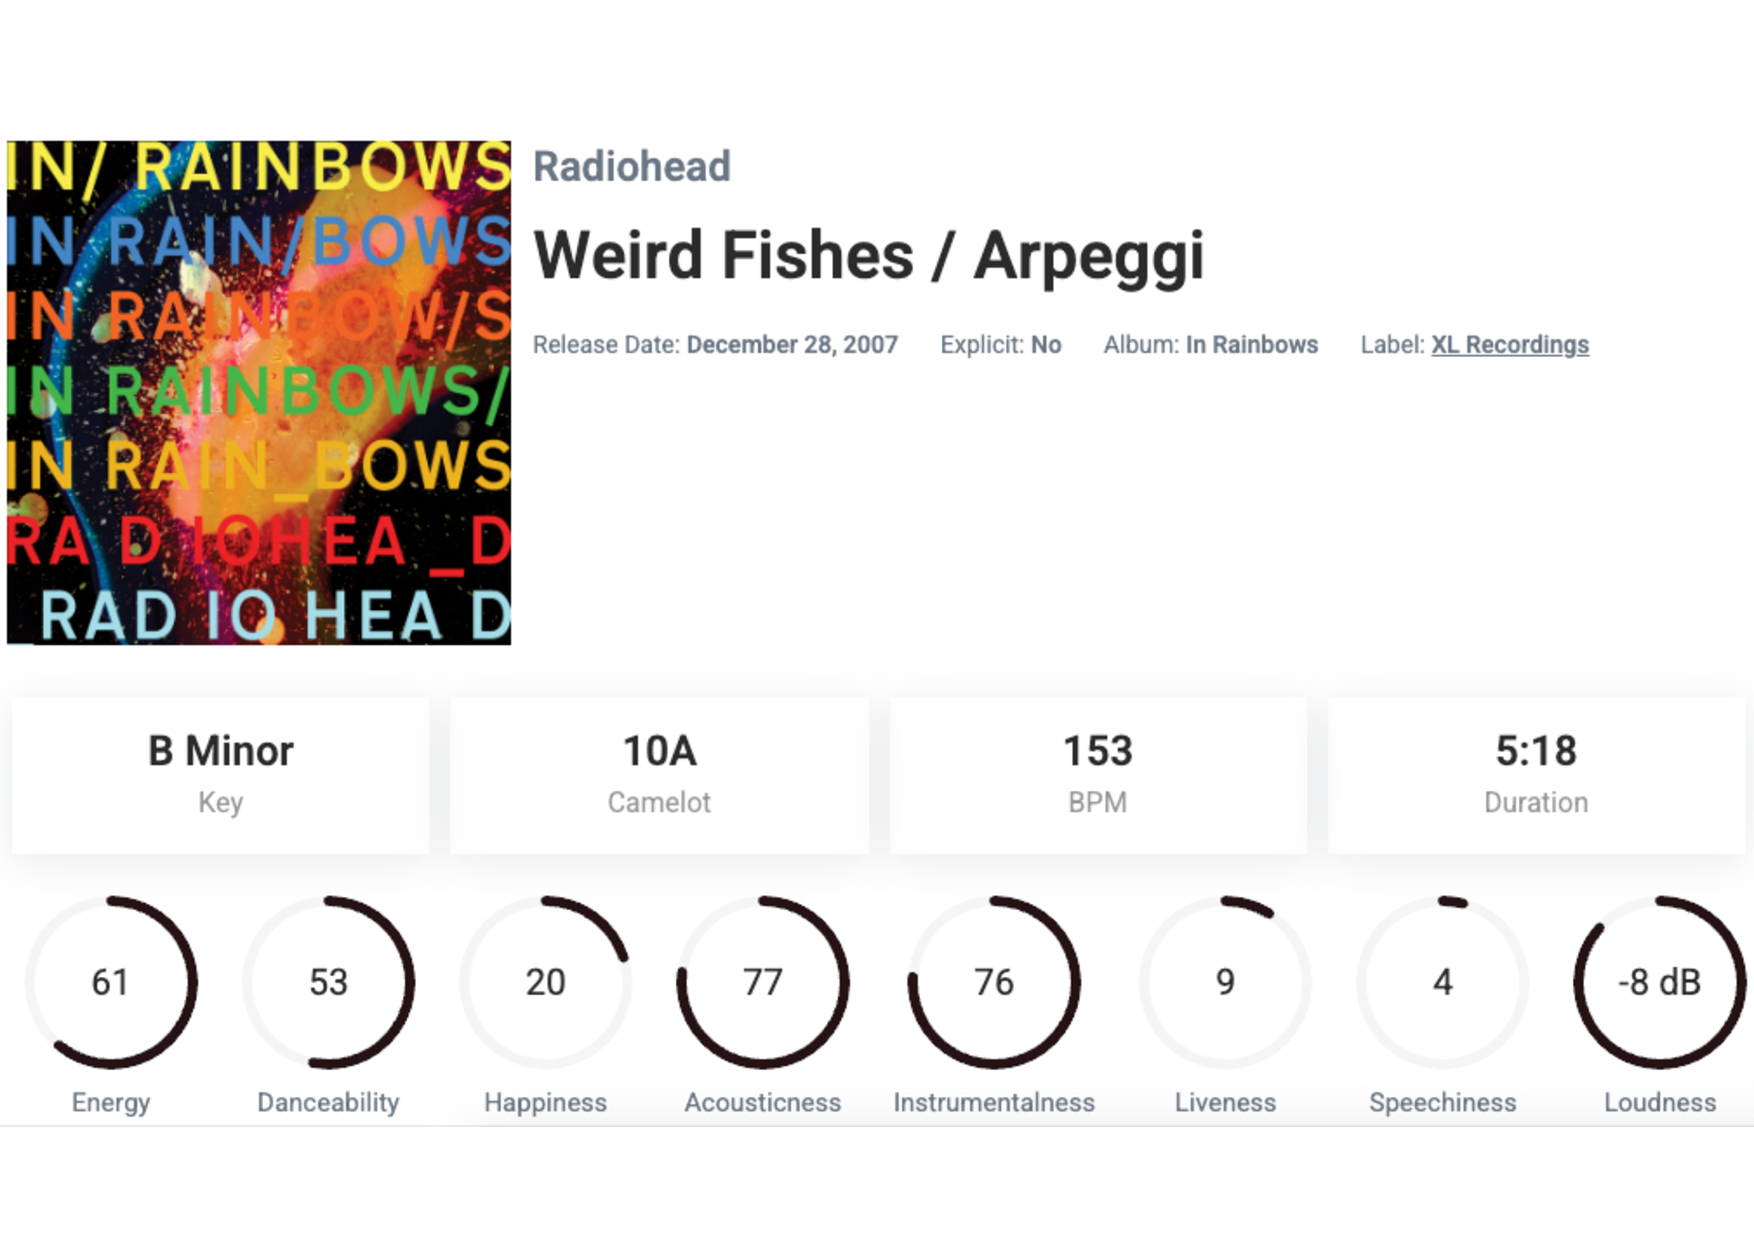
\includegraphics[width=1\textwidth]{Figures/weirdfishes.pdf}
    \caption[Interfaz de consulta en Tunebat]{Ejemplo de visualización de características musicales en Tunebat\protect\footnotemark.}
    \label{fig:tunebat_screenshot}
\end{figure}
\footnotetext{Imagen tomada de \url{https://bit.ly/4nJ8RWg}}
% \subsection{Carpetas}

\subsection{Síntesis comparativa}
\label{subsec:sintesis_estado_arte}

Las tecnologías existentes ofrecen herramientas útiles para el objetivo del trabajo. Las bibliotecas de procesamiento digital de señales permiten extraer representaciones numéricas de las ondas sonoras, y los modelos preentrenados ofrecen representaciones semánticas. Por otro lado, las soluciones comerciales proveen servicios de etiquetado para canciones.
 
Sin embargo, persisten limitaciones operativas para su aplicación directa en el entorno de la empresa. Los servicios de terceros generan costos recurrentes, limitan la cantidad de consultas y crean dependencia tecnológica. Las plataformas web de uso manual no son viables para procesar catálogos con miles de canciones. Además, los modelos no coinciden con las características y las clases específicas que usa Plusyc Live.

Por estos motivos, resulta necesario desarrollar una solución propia. El propósito de este trabajo es aprovechar las técnicas actuales de inteligencia artificial para crear un sistema independiente. Esto permite analizar directamente los archivos de audio, etiquetarlos según las necesidades de la empresa y así reducir la dependencia de proveedores externos.



% Esta plantilla se distribuye como una único archivo .zip que se puede descomprimir en varios archivos y carpetas. Asimismo, se puede consultar el repositorio git para obtener la última versión de los archivos, \url{https://github.com/patriciobos/Plantilla-CESE.git}. Los nombres de las carpetas son, o pretender ser, auto-explicativos.

% \keyword{Appendices} -- Esta es la carpeta donde se deben poner los apéndices. Cada apéndice debe ir en su propio archivo \file{.tex}. Se incluye un ejemplo y una plantilla en la carpeta.

% \keyword{Chapters} -- Esta es la carpeta donde se deben poner los capítulos de la memoria. Cada capítulo debe ir un su propio archivo \file{.tex} por separado.  Se ofrece por defecto, la siguiente estructura de capítulos y se recomienda su utilización dentro de lo posible:

% \begin{itemize}
% \item Capítulo 1: Introducción general	
% \item Capítulo 2: Introducción específica
% \item Capítulo 3: Diseño e implementación
% \item Capítulo 4: Ensayos y resultados
% \item Capítulo 5: Conclusiones

% \end{itemize}

% Esta estructura de capítulos es la que se recomienda para las memorias de la especialización.

% \keyword{Figures} -- Esta carpeta contiene todas las figuras de la memoria.  Estas son las versiones finales de las imágenes que van a ser incluidas en la memoria.  Pueden ser imágenes en formato \textit{raster}\footnote{\url{https://en.wikipedia.org/wiki/Raster_graphics}} como \file{.png}, \file{.jpg} o en formato vectoriales\footnote{\url{https://en.wikipedia.org/wiki/Vector_graphics}} como \file{.pdf}, \file{.ps}.  Se debe notar que utilizar imágenes vectoriales disminuye notablemente el peso del documento final y acelera el tiempo de compilación por lo que es recomendable su utilización siempre que sea posible.

% \subsection{Archivos}

% También están incluidos varios archivos, la mayoría de ellos son de texto plano y se puede ver su contenido en un editor de texto. Después de la compilación inicial, se verá que más archivos auxiliares son creados por \ LaTeX{} o BibTeX, pero son de uso interno y no es necesario hacer nada en particular con ellos.  Toda la información necesaria para compilar el documento se encuentra en los archivos \file{.tex}, \file{.bib}, \file{.cls} y en las imágenes de la carpeta Figures.

% \keyword{referencias.bib} - este es un archivo importante que contiene toda la información de referencias bibliográficas que se utilizarán para las citas en la memoria en conjunto con BibTeX. Usted puede escribir las entradas bibliográficas en forma manual, aunque existen también programas de gestión de referencias que facilitan la creación y gestión de las referencias y permiten exportarlas en formato BibTeX.  También hay disponibles sitios web como \url{books.google.com} que permiten obtener toda la información necesaria para una cita en formato BibTeX. Ver sección \ref{sec:biblio}

% \keyword{MastersDoctoralThesis.cls} -- este es un archivo importante. Es el archivos con la clase que le informa a \LaTeX{} cómo debe dar formato a la memoria. El usuario de la plantilla no debería necesitar modificar nada de este archivo.

% \keyword{memoria.pdf} -- esta es su memoria con una tipografía bellamente compuesta (en formato de archivo PDF) creado por \LaTeX{}. Se distribuye con la plantilla y después de compilar por primera vez sin hacer ningún cambio se debería obtener una versión idéntica a este documento.

% \keyword{memoria.tex} -- este es un archivo importante. Este es el archivo que tiene que compilar \LaTeX{} para producir la memoria como un archivo PDF. Contiene un marco de trabajo y estructuras que le indican a \LaTeX{} cómo diagramar la memoria.  Está altamente comentado para que se pueda entender qué es lo que realiza cada línea de código y por qué está incluida en ese lugar.  En este archivo se debe completar la información personalizada de las primeras sección según se indica en la sección \ref{sec:FillingFile}.

% Archivos que \emph{no} forman parte de la distribución de la plantilla pero que son generados por \LaTeX{} como archivos auxiliares necesarios para la producción de la memoria.pdf son:

% \keyword{memoria.aux} -- este es un archivo auxiliar generado por \LaTeX{}, si se borra \LaTeX{} simplemente lo regenera cuando se compila el archivo principal \file{memoria.tex}.

% \keyword{memoria.bbl} -- este es un archivo auxiliar generado por BibTeX, si se borra BibTeX simplemente lo regenera cuando se compila el archivo principal \file{memoria.tex}. Mientras que el archivo \file{.bib} contiene todas las referencias que hay, este archivo \file{.bbl} contine sólo las referencias que han sido citadas y se utiliza para la construcción de la bibiografía.

% \keyword{memoria.blg} -- este es un archivo auxiliar generado por BibTeX, si se borra BibTeX simplemente lo regenera cuando se compila el archivo principal \file{memoria.tex}.

% \keyword{memoria.lof} -- este es un archivo auxiliar generado por \LaTeX{}, si se borra \LaTeX{} simplemente lo regenera cuando se compila el archivo principal \file{memoria.tex}.  Le indica a \LaTeX{} cómo construir la sección \emph{Lista de Figuras}.
 
% \keyword{memoria.log} --  este es un archivo auxiliar generado por \LaTeX{}, si se borra \LaTeX{} simplemente lo regenera cuando se compila el archivo principal \file{memoria.tex}. Contiene mensajes de \LaTeX{}. Si se reciben errores o advertencias durante la compilación, se guardan en este archivo \file{.log}.

% \keyword{memoria.lot} -- este es un archivo auxiliar generado por \LaTeX{}, si se borra \LaTeX{} simplemente lo regenera cuando se compila el archivo principal \file{memoria.tex}.  Le indica a \LaTeX{} cómo construir la sección \emph{Lista de Tablas}.

% \keyword{memoria.out} -- este es un archivo auxiliar generado por \LaTeX{}, si se borra \LaTeX{} simplemente lo regenera cuando se compila el archivo principal \file{memoria.tex}.

% De esta larga lista de archivos, sólo aquellos con la extensión \file{.bib}, \file{.cls} y \file{.tex} son importantes.  Los otros archivos auxiliares pueden ser ignorados o borrados ya que \LaTeX{} y BibTeX los regenerarán durante la compilación.

%----------------------------------------------------------------------------------------


% \subsection{Paquetes adicionales}

% Si bien durante el proceso de instalación de TexMaker, o cualquier otro editor que se haya elegido, se instalarán en el sistema los paquetes básicos necesarios para trabajar con \LaTeX{}, la plantilla de los trabajos de Especialización y Maestría requieren de paquete adicionales.

% Se indican a continuación los comandos que se deben introducir en la consola de Ubuntu (ctrl + alt + t) para instalarlos:

% \begin{lstlisting}[language=bash]
%   $ sudo apt install texlive-lang-spanish texlive-science 
%   $ sudo apt install texlive-bibtex-extra biber
%   $ sudo apt install texlive texlive-fonts-recommended
%   $ sudo apt install texlive-latex-extra
% \end{lstlisting}


% \subsection{Configurando TexMaker}
% \label{subsec:configurando}



% Una vez instalado el programa y los paquetes adicionales se debe abrir el archivo memoria.tex con el editor para ver una pantalla similar a la que se puede apreciar en la figura \ref{fig:texmaker}. 
% Una vez instalado el programa y los paquetes adicionales se debe abrir el archivo memoria.tex con el editor para ver una pantalla similar a la que se puede apreciar en la figura \ref{fig:texmaker}. 
% Una vez instalado el programa y los paquetes adicionales se debe abrir el archivo memoria.tex con el editor para ver una pantalla similar a la que se puede apreciar en la figura \ref{fig:texmaker}. 
% Una vez instalado el programa y los paquetes adicionales se debe abrir el archivo memoria.tex con el editor para ver una pantalla similar a la que se puede apreciar en la figura \ref{fig:texmaker}. 

% \vspace{1cm}

% \begin{figure}[htbp]
% 	\centering
% 	\includegraphics[width=.5\textwidth]{./Figures/texmaker.png}
% 	\caption{Entorno de trabajo de texMaker.}
% 	\label{fig:texmaker}
% \end{figure}

% \vspace{1cm}

% Notar que existe una vista llamada Estructura a la izquierda de la interfaz que nos permite abrir desde dentro del programa los archivos individuales de los capítulos.  A la derecha se encuentra una vista con el archivo propiamente dicho para su edición. Hacia la parte inferior se encuentra una vista del log con información de los resultados de la compilación.  En esta última vista pueden aparecen advertencias o \textit{warning}, que normalmente pueden ser ignorados, y los errores que se indican en color rojo y deben resolverse para que se genere el PDF de salida.

% Recordar que el archivo que se debe compilar con PDFLaTeX es \file{memoria.tex}, si se tratara de compilar alguno de los capítulos saldría un error.  Para salvar la molestia de tener que cambiar de archivo para compilar cada vez que se realice una modificación en un capítulo, se puede definir el archivo \file{memoria.tex} como ``documento maestro'' yendo al menú opciones -> ``definir documento actual como documento maestro'', lo que permite compilar con PDFLaTeX memoria.tex directamente desde cualquier archivo que se esté modificando . Se muestra esta opción en la figura \ref{fig:docMaestro}.

% \begin{figure}[h]
% 	\centering
% 	\includegraphics[width=\textwidth]{./Figures/docMaestro.png}
% 	\caption{Definir memoria.tex como documento maestro.}
% 	\label{fig:docMaestro}
% \end{figure}

% En el menú herramientas se encuentran las opciones de compilación.  Para producir un archivo PDF a partir de un archivo .tex se debe ejecutar PDFLaTeX (el shortcut es F6). Para incorporar nueva bibliografía se debe utilizar la opción BibTeX del mismo menú herramientas (el shortcut es F11).

% Notar que para actualizar las tablas de contenidos se debe ejecutar PDFLaTeX dos veces.  Esto se debe a que es necesario actualizar algunos archivos auxiliares antes de obtener el resultado final.  En forma similar, para actualizar las referencias bibliográficas se debe ejecutar primero PDFLaTeX, después BibTeX y finalmente PDFLaTeX dos veces por idénticos motivos.

% \section{Personalizando la plantilla, el archivo \file{memoria.tex}}
% \label{sec:FillingFile}

% Para personalizar la plantilla se debe incorporar la información propia en los distintos archivos \file{.tex}. 

% Primero abrir \file{memoria.tex} con TexMaker (o el editor de su preferencia). Se debe ubicar dentro del archivo el bloque de código titulado \emph{INFORMACIÓN DE LA PORTADA} donde se deben incorporar los primeros datos personales con los que se construirá automáticamente la portada.


%----------------------------------------------------------------------------------------

% \section{El código del archivo \file{memoria.tex} explicado}

% El archivo \file{memoria.tex} contiene la estructura del documento y es el archivo de mayor jerarquía de la memoria.  Podría ser equiparable a la función \emph{main()} de un programa en C, o mejor dicho al archivo fuente .c donde se encuentra definida la función main().

% La estructura básica de cualquier documento de \LaTeX{} comienza con la definición de clase del documento, es seguida por un preámbulo donde se pueden agregar funcionalidades con el uso de \texttt{paquetes} (equiparables a bibliotecas de C), y finalmente, termina con el cuerpo del documento, donde irá el contenido de la memoria.

% \lstset{%
%   basicstyle=\small\ttfamily,
%   language=[LaTeX]{TeX}
% }

% \begin{lstlisting}
% \documentclass{article}  <- Definicion de clase
% \usepackage{listings}	 <- Preambulo

% \begin{document}	 <- Comienzo del contenido propio 
% 	Hello world!
% \end{document}
% \end{lstlisting}


% El archivo \file{memoria.tex} se encuentra densamente comentado para explicar qué páginas, secciones y elementos de formato está creando el código \LaTeX{} en cada línea. El código está dividido en bloques con nombres en mayúsculas para que resulte evidente qué es lo que hace esa porción de código en particular. Inicialmente puede parecer que hay mucho código \LaTeX{}, pero es principalmente código para dar formato a la memoria por lo que no requiere intervención del usuario de la plantilla.  Sí se deben personalizar con su información los bloques indicados como:

% \begin{itemize}
% 	\item Informacion de la memoria
% 	\item Resumen
% 	\item Agradecimientos
% 	\item Dedicatoria
% \end{itemize}

% El índice de contenidos, las listas de figura de tablas se generan en forma automática y no requieren intervención ni edición manual por parte del usuario de la plantilla. 

% En la parte final del documento se encuentran los capítulos y los apéndices.  Por defecto se incluyen los 5 capítulos propuestos que se encuentran en la carpeta /Chapters. Cada capítulo se debe escribir en un archivo .tex separado y se debe poner en la carpeta \emph{Chapters} con el nombre \file{Chapter1}, \file{Chapter2}, etc\ldots El código para incluir capítulos desde archivos externos se muestra a continuación.

% \begin{verbatim}
% 	\include{Chapters/Chapter1}
% 	\include{Chapters/Chapter2} 
% 	\include{Chapters/Chapter3}
% 	\include{Chapters/Chapter4} 
% 	\include{Chapters/Chapter5} 
% \end{verbatim}

% Los apéndices también deben escribirse en archivos .tex separados, que se deben ubicar dentro de la carpeta \emph{Appendices}. Los apéndices vienen comentados por defecto con el caracter \code{\%} y para incluirlos simplemente se debe eliminar dicho caracter.

% Finalmente, se encuentra el código para incluir la bibliografía en el documento final.  Este código tampoco debe modificarse. La metodología para trabajar las referencias bibliográficas se desarrolla en la sección \ref{sec:biblio}.
%----------------------------------------------------------------------------------------

% \section{Bibliografía}
% \label{sec:biblio}

% Las opciones de formato de la bibliografía se controlan a través del paquete de latex \option{biblatex} que se incluye en la memoria en el archivo memoria.tex.  Estas opciones determinan cómo se generan las citas bibliográficas en el cuerpo del documento y cómo se genera la bibliografía al final de la memoria.

% En el preámbulo se puede encontrar el código que incluye el paquete biblatex, que no requiere ninguna modificación del usuario de la plantilla, y que contiene las siguientes opciones:

% \begin{lstlisting}
% \usepackage[backend=bibtex,
% 	natbib=true, 
% 	style=numeric, 
% 	sorting=none]
% {biblatex}
% \end{lstlisting}

% En el archivo \file{reference.bib} se encuentran las referencias bibliográficas que se pueden citar en el documento.  Para incorporar una nueva cita al documento lo primero es agregarla en este archivo con todos los campos necesario.  Todas las entradas bibliográficas comienzan con $@$ y una palabra que define el formato de la entrada.  Para cada formato existen campos obligatorios que deben completarse. No importa el orden en que las entradas estén definidas en el archivo .bib.  Tampoco es importante el orden en que estén definidos los campos de una entrada bibliográfica. A continuación se muestran algunos ejemplos:

% \begin{lstlisting}
% @ARTICLE{ARTICLE:1,
%     AUTHOR="John Doe",
%     TITLE="Title",
%     JOURNAL="Journal",
%     YEAR="2017",
% }
% \end{lstlisting}


% \begin{lstlisting}
% @BOOK{BOOK:1,
%     AUTHOR="John Doe",
%     TITLE="The Book without Title",
%     PUBLISHER="Dummy Publisher",
%     YEAR="2100",
% }
% \end{lstlisting}


% \begin{lstlisting}
% @INBOOK{BOOK:2,
%     AUTHOR="John Doe",
%     TITLE="The Book without Title",
%     PUBLISHER="Dummy Publisher",
%     YEAR="2100",
%     PAGES="100-200",
% }
% \end{lstlisting}


% \begin{lstlisting}
% @MISC{WEBSITE:1,
%     HOWPUBLISHED = "\url{http://example.com}",
%     AUTHOR = "Intel",
%     TITLE = "Example Website",
%     MONTH = "12",
%     YEAR = "1988",
%     URLDATE = {2012-11-26}
% }
% \end{lstlisting}

% Se debe notar que los nombres \emph{ARTICLE:1}, \emph{BOOK:1}, \emph{BOOK:2} y \emph{WEBSITE:1} son nombres de fantasía que le sirve al autor del documento para identificar la entrada. En este sentido, se podrían reemplazar por cualquier otro nombre.  Tampoco es necesario poner : seguido de un número, en los ejemplos sólo se incluye como un posible estilo para identificar las entradas.

% La entradas se citan en el documento con el comando: 

% \begin{verbatim}
% \citep{nombre_de_la_entrada}
% \end{verbatim}

% Y cuando se usan, se muestran así: \citep{ARTICLE:1}, \citep{BOOK:1}, \citep{BOOK:2}, \citep{WEBSITE:1}.  Notar cómo se conforma la sección Bibliografía al final del documento.

% Finalmente y como se mencionó en la subsección \ref{subsec:configurando}, para actualizar las referencias bibliográficas tanto en la sección bibliografía como las citas en el cuerpo del documento, se deben ejecutar las herramientas de compilación PDFLaTeX, BibTeX, PDFLaTeX, PDFLaTeX, en ese orden.  Este procedimiento debería resolver cualquier mensaje "Citation xxxxx on page x undefined".

% 	\chapter{Introducción específica} % Main chapter title

\label{Chapter2}

%----------------------------------------------------------------------------------------
%	SECTION 1
%----------------------------------------------------------------------------------------
Este capítulo introduce las herramientas de terceros y las tecnologías necesarias para el desarrollo del sistema. Se describe la fuente de datos principal, las técnicas para extraer representaciones numéricas del audio, los modelos predictivos y las tecnologías utilizadas para el despliegue.

\section{Fuentes de datos de canciones}
\label{sec:datos}

Para el entrenamiento de los modelos predictivos se utilizó la colección privada de canciones de la empresa. Esta fuente de datos cuenta con más de 60~000 archivos de audio de canciones completas.

Se seleccionó este conjunto de datos por la disponibilidad en el acceso a la información y por su representatividad en ambientes comerciales reales. Por el contrario, otros conjuntos de datos públicos musicales, como GTZAN \citep{GTZAN} y los subconjuntos estándar de FMA \citep{FMA}, ofrecen fragmentos limitados a 10 o 30 segundos de audio. El uso de pistas incompletas restringe la disponibilidad de la información musical. Realizar predicciones sobre el audio total resulta más preciso, ya que evita la pérdida de los eventos musicales que ocurren antes o después de una sola ventana. Además, estas alternativas carecen parcialmente de las variables objetivo requeridas en el alcance del trabajo.

El acceso a los archivos de audio de canciones completas garantiza la preservación de la estructura musical, evita la pérdida de información y flexibiliza la extracción de representaciones matemáticas mediante el uso de bibliotecas y modelos preentrenados.

El análisis comparativo de las fuentes de datos, las representaciones estadísticas de las canciones y los criterios de selección de variables predictivas se detallan en el Capítulo 3.
% TODO: Cambiar "Capítulo 3" por las referencias cruzadas (\ref{}) de las secciones exactas una vez que se termine de escribir el Capítulo 3.

\section{Representaciones numéricas de la música}
\label{sec:dsp}

Una canción se traduce a un formato numérico para su procesamiento computacional. El procesamiento digital de señales (DSP) transforma la onda sonora en arreglos matemáticos de una o dos dimensiones. 
Entre las representaciones bidimensionales más destacadas se encuentran el espectrograma, el cromagrama y el espacio armónico o tonnetz. El espectrograma refleja la variación de las frecuencias a lo largo del tiempo. Por su parte, el cromagrama captura la energía asociada a las doce clases de notas musicales. Finalmente, el tonnetz modela las relaciones tonales y armónicas de la pista. A modo de ejemplo, en la figura \ref{fig:representaciones_2d} se ilustran estas tres transformaciones aplicadas a un fragmento de la canción ``Weird Fishes/Arpeggi'' de la banda Radiohead. En estos gráficos, el eje horizontal representa el tiempo, mientras que la intensidad del color indica la magnitud de la energía para las distintas frecuencias, notas musicales o relaciones tonales correspondientes a cada eje vertical.

\begin{figure}[htpb]
    \centering
    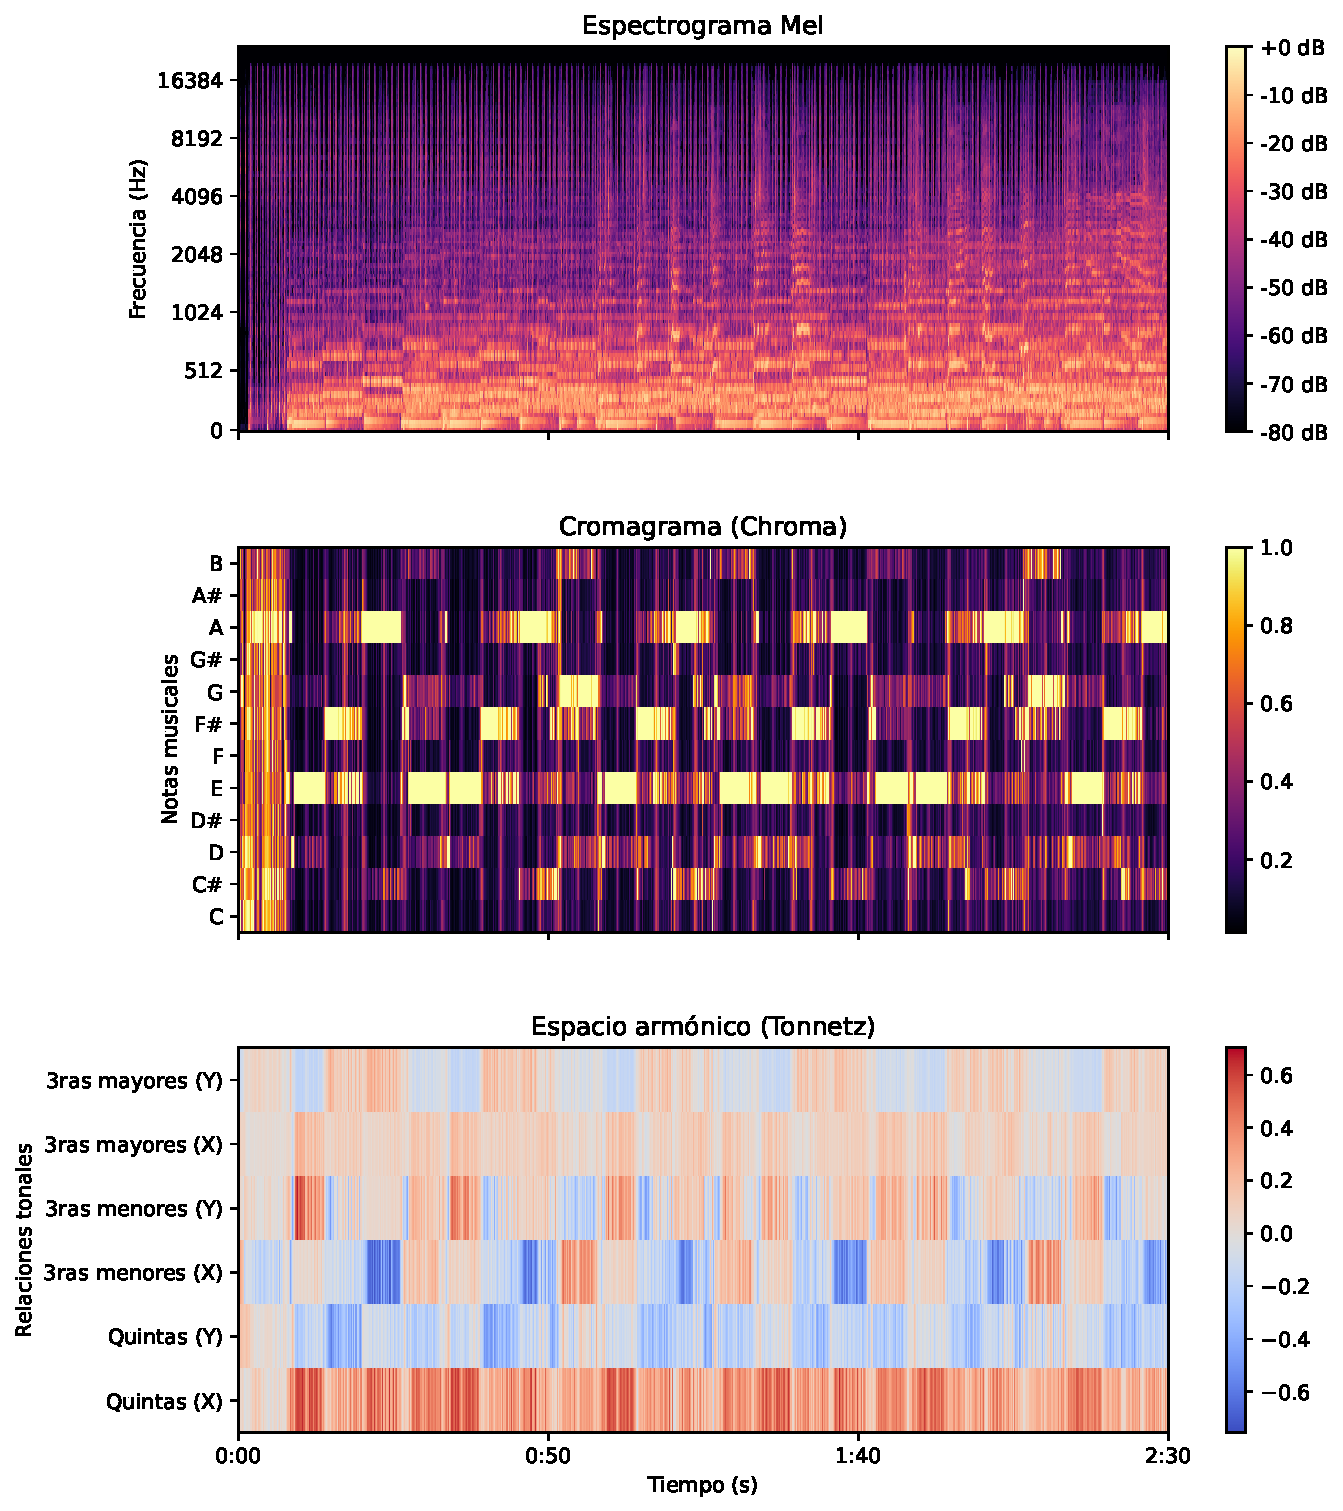
\includegraphics[width=1\textwidth]{./Figures/espectro_croma_tonnetz.pdf}
    \caption[Representaciones visuales del audio]{Representación visual de un espectrograma, un cromagrama y un tonnetz.}
    \label{fig:representaciones_2d}
\end{figure}

Además de las representaciones bidimensionales, las bibliotecas de procesamiento de señales facilitan la extracción de atributos numéricos unidimensionales. En la tabla \ref{tab:atributos_dsp} se presenta un listado que introduce algunas de las características de bajo nivel más representativas en el análisis musical. En la elaboración del trabajo se usaron Librosa y Essentia en este proceso.

Estas transformaciones matemáticas reducen la dimensionalidad del archivo de audio. Sin embargo, carecen de significado semántico. Su función principal, en el contexto de este trabajo, es la de generar las variables predictivas necesarias para entrenar modelos de aprendizaje automático.

El listado completo de las variables de entrada, el análisis de su relevancia y su impacto en el rendimiento de los algoritmos se detalla en el Capítulo 3.

\begin{table}[htpb]
    \centering
    \caption[Atributos representativos]{Listado introductorio de los principales atributos de procesamiento de señales extraídos del audio.}
    \renewcommand{\arraystretch}{1.2}
    \begin{tabular}{p{3.5cm} p{8.5cm}}    
        \toprule
        \textbf{Atributo} & \textbf{Descripción principal} \\
        \midrule
        MFCC & Coeficientes cepstrales que modelan la percepción auditiva humana. \\       
        Centroide espectral & Indica el centro de masa del espectro acústico. Se asocia al brillo del sonido. \\
        Ancho de banda & Mide la dispersión de las frecuencias alrededor del centroide espectral. \\
        Tasa de cruces por cero & Cuantifica la cantidad de cambios de signo en la señal temporal. \\
        Rolloff espectral & Estima la frecuencia por debajo de la que se concentra la mayor parte de la energía. \\
        \bottomrule
    \end{tabular}
    \label{tab:atributos_dsp}
\end{table}

\section{Información semántica del audio}
\label{sec:semantica}

Las representaciones de bajo nivel descritas en la sección 2.2 no siempre son suficientes para capturar conceptos musicales complejos. Es posible mejorar la cobertura de la información musical con el aprendizaje por transferencia. Esta técnica consiste en utilizar modelos previamente entrenados con grandes volúmenes de datos para extraer características semánticas de alto nivel.

Para este fin existen bibliotecas especializadas, como PANNs Inference. Esta herramienta provee acceso a redes neuronales optimizadas para el análisis de eventos sonoros. Dentro de sus opciones, destaca la arquitectura denominada CNN14 \citep{kong2020panns}. Se trata de una red neuronal convolucional, capaz de abstraer patrones del audio y generar embeddings numéricos basados en las clases del conjunto de datos AudioSet. 

Un ejemplo de las probabilidades de detección obtenidas para distintas clases de eventos sonoros a lo largo del tiempo se visualiza en la figura \ref{fig:mapa_semantico}, donde se muestran ventanas consecutivas de 10 segundos de la canción de Radiohead. En este mapa de calor, las áreas más claras indican una mayor probabilidad de activación para cada clase.

El uso de esta arquitectura permite transformar la onda sonora para extraer embeddings y obtener probabilidades asociadas a etiquetas predefinidas, como la presencia de aplausos, instrumentos musicales específicos o habla. Estos datos semánticos enriquecen el conjunto de variables de entrada para la inferencia de algunas de las características musicales que se definieron en el alcance del trabajo.

\newpage
\begin{figure}[!htpb]
    \centering
    
\includegraphics[width=1\textwidth]{mapa_top_clases.pdf}
    \caption[Probabilidades de detección semántica]{Mapa de calor de las características semánticas extraídas mediante la red CNN14.}
    \label{fig:mapa_semantico}
\end{figure}

\section{Modelos de inteligencia artificial utilizados}
\label{sec:modelos}

Una vez obtenidos los descriptores numéricos y semánticos, es necesario aplicar algoritmos de predicción. Para este fin, se utilizaron dos enfoques principales:

\begin{itemize}
    \item Algoritmos LightGBM: se integró la arquitectura LightGBM, basada en el ensamble de árboles de decisión. Esta herramienta destaca por su alta velocidad computacional y eficiencia en tareas generales de predicción.
    \item Redes MLP: los perceptrones multicapa son redes neuronales artificiales con capacidad para modelar relaciones complejas. Permiten, entre otras aplicaciones, predecir múltiples variables continuas de forma simultánea.
\end{itemize}

\section{Despliegue e integración}
\label{sec:despliegue}

La integración del sistema predictivo requirió del despliegue de una interfaz de programación de aplicaciones. Para su construcción se utilizó FastAPI \citep{ramirez2018fastapi} como marco de trabajo. Esta herramienta facilita el desarrollo de servicios web de alto rendimiento basados en Python \citep{python3}.

El alojamiento remoto del producto se apoyó en los servicios de infraestructura de OCI (por su sigla en inglés, Oracle Cloud Infrastructure) \citep{oracle_oci}. Se provisionó una instancia de cómputo virtual en la nube para desplegar la aplicación y ejecutar los modelos predictivos. El uso de esta tecnología garantiza la disponibilidad continua del sistema.

%     \centering
%     \includegraphics[width=0.9\textwidth]{./Figures/diagrama_bloques.pdf}
%     \caption{Diagrama de bloques del sistema en su entorno de despliegue en la nube.}
%     \label{fig:diagrama_despliegue}
% \end{figure}


% \subsection{Uso de mayúscula inicial para los título de secciones}

% Si en el texto se hace alusión a diferentes partes del trabajo referirse a ellas como capítulo, sección o subsección según corresponda. Por ejemplo: ``En el capítulo \ref{Chapter1} se explica tal cosa'', o ``En la sección \ref{sec:ejemplo} se presenta lo que sea'', o ``En la subsección \ref{subsec:ejemplo} se discute otra cosa''.

% Cuando se quiere poner una lista tabulada, se hace así:

% \begin{itemize}
% 	\item Este es el primer elemento de la lista.
% 	\item Este es el segundo elemento de la lista.
% \end{itemize}

% Notar el uso de las mayúsculas y el punto al final de cada elemento.

% Si se desea poner una lista numerada el formato es este:

% \begin{enumerate}
% 	\item Este es el primer elemento de la lista.
% 	\item Este es el segundo elemento de la lista.
% \end{enumerate}

% Notar el uso de las mayúsculas y el punto al final de cada elemento.

% \subsection{Este es el título de una subsección}
% \label{subsec:ejemplo}

% Se recomienda no utilizar \textbf{texto en negritas} en ningún párrafo, ni tampoco texto \underline{subrayado}. En cambio sí se debe utilizar \textit{texto en itálicas} para palabras en un idioma extranjero, al menos la primera vez que aparecen en el texto. En el caso de palabras que estamos inventando se deben utilizar ``comillas'', así como también para citas textuales. Por ejemplo, un \textit{digital filter} es una especie de ``selector'' que permite separar ciertos componentes armónicos en particular.

% La escritura debe ser impersonal. Por ejemplo, no utilizar ``el diseño del firmware lo hice de acuerdo con tal principio'', sino ``el firmware fue diseñado utilizando tal principio''. 

% El trabajo es algo que al momento de escribir la memoria se supone que ya está concluido, entonces todo lo que se refiera a hacer el trabajo se narra en tiempo pasado, porque es algo que ya ocurrió. Por ejemplo, "se diseñó el firmware empleando la técnica de test driven development".

% En cambio, la memoria es algo que está vivo cada vez que el lector la lee. Por eso transcurre siempre en tiempo presente, como por ejemplo:

% ``En el presente capítulo se da una visión global sobre las distintas pruebas realizadas y los resultados obtenidos. Se explica el modo en que fueron llevados a cabo los test unitarios y las pruebas del sistema''.

% Se recomienda no utilizar una sección de glosario sino colocar la descripción de las abreviaturas como parte del mismo cuerpo del texto. Por ejemplo, RTOS (\textit{Real Time Operating System}, Sistema Operativo de Tiempo Real) o en caso de considerarlo apropiado mediante notas a pie de página.

% Si se desea indicar alguna página web utilizar el siguiente formato de referencias bibliográficas, dónde las referencias se detallan en la sección de bibliografía de la memoria, utilizado el formato establecido por IEEE en \citep{IEEE:citation}. Por ejemplo, ``el presente trabajo se basa en la plataforma EDU-CIAA-NXP \citep{CIAA}, la cual...''.

% \subsection{Figuras} 

% Al insertar figuras en la memoria se deben considerar determinadas pautas. Para empezar, usar siempre tipografía claramente legible. Luego, tener claro que \textbf{es incorrecto} escribir por ejemplo esto: ``El diseño elegido es un cuadrado, como se ve en la siguiente figura:''

% \begin{figure}[h]
% \centering
% \includegraphics[scale=.45]{./Figures/cuadradoAzul.png}
% \end{figure}

% La forma correcta de utilizar una figura es con referencias cruzadas, por ejemplo: ``Se eligió utilizar un cuadrado azul para el logo, como puede observarse en la figura \ref{fig:cuadradoAzul}''.

% \begin{figure}[ht]
% 	\centering
% 	\includegraphics[scale=.45]{./Figures/cuadradoAzul.png}
% 	\caption{Ilustración del cuadrado azul que se eligió para el diseño del logo.}
% 	\label{fig:cuadradoAzul}
% \end{figure}

% El texto de las figuras debe estar siempre en español, excepto que se decida reproducir una figura original tomada de alguna referencia. En ese caso la referencia de la cual se tomó la figura debe ser indicada en el epígrafe de la figura e incluida como una nota al pie, como se ilustra en la figura \ref{fig:palabraIngles}.

% \begin{figure}[htpb]
% 	\centering
% 	\includegraphics[scale=.3]{./Figures/word.jpeg}
% 	\caption{Imagen tomada de la página oficial del procesador\protect\footnotemark.}
% 	\label{fig:palabraIngles}
% \end{figure}

% \footnotetext{Imagen tomada de \url{https://goo.gl/images/i7C70w}}

% La figura y el epígrafe deben conformar una unidad cuyo significado principal pueda ser comprendido por el lector sin necesidad de leer el cuerpo central de la memoria. Para eso es necesario que el epígrafe sea todo lo detallado que corresponda y si en la figura se utilizan abreviaturas entonces aclarar su significado en el epígrafe o en la misma figura.



% \begin{figure}[ht]
% 	\centering
% 	\includegraphics[scale=.37]{./Figures/questionMark.png}
% 	\caption{¿Por qué de pronto aparece esta figura?}
% 	\label{fig:questionMark}
% \end{figure}

% Nunca colocar una figura en el documento antes de hacer la primera referencia a ella, como se ilustra con la figura \ref{fig:questionMark}, porque sino el lector no comprenderá por qué de pronto aparece la figura en el documento, lo que distraerá su atención.

% Otra posibilidad es utilizar el entorno \textit{subfigure} para incluir más de una figura, como se puede ver en la figura \ref{fig:three graphs}. Notar que se pueden referenciar también las figuras internas individualmente de esta manera: \ref{fig:1de3}, \ref{fig:2de3} y \ref{fig:3de3}.
 
% \begin{figure}[!htpb]
%      \centering
%      \begin{subfigure}[b]{0.3\textwidth}
%          \centering
%          \includegraphics[width=.65\textwidth]{./Figures/questionMark}
%          \caption{Un caption.}
%          \label{fig:1de3}
%      \end{subfigure}
%      \hfill
%      \begin{subfigure}[b]{0.3\textwidth}
%          \centering
%          \includegraphics[width=.65\textwidth]{./Figures/questionMark}
%          \caption{Otro.}
%          \label{fig:2de3}
%      \end{subfigure}
%      \hfill
%      \begin{subfigure}[b]{0.3\textwidth}
%          \centering
%          \includegraphics[width=.65\textwidth]{./Figures/questionMark}
%          \caption{Y otro más.}
%          \label{fig:3de3}
%      \end{subfigure}
%         \caption{Tres gráficos simples.}
%         \label{fig:three graphs}
% \end{figure}

% El código para generar las imágenes se encuentra disponible para su reutilización en el archivo \file{Chapter2.tex}.

% \subsection{Tablas}

% Para las tablas utilizar el mismo formato que para las figuras, sólo que el epígrafe se debe colocar arriba de la tabla, como se ilustra en la tabla \ref{tab:peces}. Observar que sólo algunas filas van con líneas visibles y notar el uso de las negritas para los encabezados.  La referencia se logra utilizando el comando \verb|\ref{<label>}| donde label debe estar definida dentro del entorno de la tabla.

% \begin{verbatim}
% \begin{table}[h]
% 	\centering
% 	\caption[caption corto]{caption largo más descriptivo}
% 	\begin{tabular}{l c c}    
% 		\toprule
% 		\textbf{Especie}     & \textbf{Tamaño} & \textbf{Valor}\\
% 		\midrule
% 		Amphiprion Ocellaris & 10 cm           & \$ 6.000 \\		
% 		Hepatus Blue Tang    & 15 cm           & \$ 7.000 \\
% 		Zebrasoma Xanthurus  & 12 cm           & \$ 6.800 \\
% 		\bottomrule
% 		\hline
% 	\end{tabular}
% 	\label{tab:peces}
% \end{table}
% \end{verbatim}


% \begin{table}[h]
% 	\centering
% 	\caption[caption corto]{caption largo más descriptivo.}
% 	\begin{tabular}{l c c}    
% 		\toprule
% 		\textbf{Especie} 	 & \textbf{Tamaño} 		& \textbf{Valor}  \\
% 		\midrule
% 		Amphiprion Ocellaris & 10 cm 				& \$ 6.000 \\		
% 		Hepatus Blue Tang	 & 15 cm				& \$ 7.000 \\
% 		Zebrasoma Xanthurus	 & 12 cm				& \$ 6.800 \\
% 		\bottomrule
% 		\hline
% 	\end{tabular}
% 	\label{tab:peces}
% \end{table}

% En cada capítulo se debe reiniciar el número de conteo de las figuras y las tablas, por ejemplo, figura 2.1 o tabla 2.1, pero no se debe reiniciar el conteo en cada sección. Por suerte la plantilla se encarga de esto por nosotros.

% \subsection{Ecuaciones}
% \label{sec:Ecuaciones}

% Al insertar ecuaciones en la memoria dentro de un entorno \textit{equation}, éstas se numeran en forma automática  y se pueden referir al igual que como se hace con las figuras y tablas, por ejemplo ver la ecuación \ref{eq:metric}.

% \begin{equation}
% 	\label{eq:metric}
% 	ds^2 = c^2 dt^2 \left( \frac{d\sigma^2}{1-k\sigma^2} + \sigma^2\left[ d\theta^2 + \sin^2\theta d\phi^2 \right] \right)
% \end{equation}
                                                        
% Para generar la ecuación \ref{eq:metric} se utilizó el siguiente código:

% \begin{verbatim}
% \begin{equation}
% 	\label{eq:metric}
% 	ds^2 = c^2 dt^2 \left( \frac{d\sigma^2}{1-k\sigma^2} + 
% 	\sigma^2\left[ d\theta^2 + 
% 	\sin^2\theta d\phi^2 \right] \right)
% \end{equation}
% \end{verbatim}
 
% 	\chapter{Diseño e implementación} % Main chapter title

\label{Chapter3} % Change X to a consecutive number; for referencing this chapter elsewhere, use \ref{ChapterX}

% Todos los capítulos deben comenzar con un breve párrafo introductorio que indique cuál es el contenido que se encontrará al leerlo.  La redacción sobre el contenido de la memoria debe hacerse en presente y todo lo referido al proyecto en pasado, siempre de modo impersonal.

\definecolor{mygreen}{rgb}{0,0.6,0}
\definecolor{mygray}{rgb}{0.5,0.5,0.5}
\definecolor{mymauve}{rgb}{0.58,0,0.82}

%%%%%%%%%%%%%%%%%%%%%%%%%%%%%%%%%%%%%%%%%%%%%%%%%%%%%%%%%%%%%%%%%%%%%%%%%%%%%
% parámetros para configurar el formato del código en los entornos lstlisting
%%%%%%%%%%%%%%%%%%%%%%%%%%%%%%%%%%%%%%%%%%%%%%%%%%%%%%%%%%%%%%%%%%%%%%%%%%%%%
\lstset{ %
  backgroundcolor=\color{white},   % choose the background color; you must add \usepackage{color} or \usepackage{xcolor}
  basicstyle=\footnotesize,        % the size of the fonts that are used for the code
  breakatwhitespace=false,         % sets if automatic breaks should only happen at whitespace
  breaklines=true,                 % sets automatic line breaking
  captionpos=b,                    % sets the caption-position to bottom
  commentstyle=\color{mygreen},    % comment style
  deletekeywords={...},            % if you want to delete keywords from the given language
  %escapeinside={\%*}{*)},          % if you want to add LaTeX within your code
  %extendedchars=true,              % lets you use non-ASCII characters; for 8-bits encodings only, does not work with UTF-8
  %frame=single,	                % adds a frame around the code
  keepspaces=true,                 % keeps spaces in text, useful for keeping indentation of code (possibly needs columns=flexible)
  keywordstyle=\color{blue},       % keyword style
  language=Python,                % the language of the code
  %otherkeywords={*,...},           % if you want to add more keywords to the set
  numbers=left,                    % where to put the line-numbers; possible values are (none, left, right)
  numbersep=5pt,                   % how far the line-numbers are from the code
  numberstyle=\tiny\color{mygray}, % the style that is used for the line-numbers
  rulecolor=\color{black},         % if not set, the frame-color may be changed on line-breaks within not-black text (e.g. comments (green here))
  showspaces=false,                % show spaces everywhere adding particular underscores; it overrides 'showstringspaces'
  showstringspaces=false,          % underline spaces within strings only
  showtabs=false,                  % show tabs within strings adding particular underscores
  stepnumber=1,                    % the step between two line-numbers. If it's 1, each line will be numbered
  stringstyle=\color{mymauve},     % string literal style
  tabsize=2,	                   % sets default tabsize to 2 spaces
  title=\lstname,                  % show the filename of files included with \lstinputlisting; also try caption instead of title
  morecomment=[s]{/*}{*/}
}


Este capítulo detalla el diseño y la implementación del sistema predictivo. Se analizan los conjuntos de datos utilizados, la extracción de atributos del audio y el tratamiento de datos según las distribuciones de las variables objetivo. Asimismo, se describen las técnicas de reducción y selección de variables, el proceso de optimización de los modelos y los resultados de la iteración productiva. Finalmente, se presenta la arquitectura desarrollada para el despliegue y la integración del sistema en un entorno operativo.

%----------------------------------------------------------------------------------------
%	SECTION 1
%----------------------------------------------------------------------------------------
\section{Conjuntos de datos}
\label{sec:conjuntos_datos}
% Aquí se describirá la extracción de datos del audio.

\subsection{Análisis de conjuntos de datos públicos}

La definición de la estrategia para la extracción de atributos se fundamenta en una revisión de conjuntos de datos públicos estandarizados en el ámbito MIR. 
El objetivo fue entender cómo repositorios de referencia, como FMA y Million Song Dataset, representan y estructuran los datos musicales, para decidir su viabilidad en el contexto de aplicación de este trabajo. 

\subsubsection{GTZAN}
Este conjunto de datos se considera el equivalente al MNIST \cite{lecun1998gradient} para el análisis de audio \cite{sturm2014state}, dada su adopción histórica como estándar de evaluación en tareas de clasificación de géneros musicales.
\begin{itemize}
    \item Variables predictivas principales: tempo, representaciones chroma, amplitud media cuadrática (RMS), descriptores espectrales y coeficientes MFCC.
    \item Estructura: 1~000 archivos de audio en crudo limitados a 30 segundos, acompañados de metadatos tabulares e imágenes de espectrogramas de Mel en su versión distribuida mediante Kaggle \citep{gtzan_kaggle}. 
    Todas estas representaciones fueron extraídas utilizando la biblioteca Librosa. Las tablas contienen los atributos calculados sobre la pista completa y también sobre divisiones de 3 segundos para incrementar el volumen de datos de entrenamiento. En ambos escenarios se aplica una reducción de dimensionalidad temporal: las variables se calculan inicialmente sobre micro-ventanas de milisegundos y luego se colapsan a valores estáticos mediante estadísticos de agregación, como la media y la varianza.
    \item Variables objetivo principales en Plusyc: se podría relacionar con \textit{suggested genres}. 
    \item Desventajas: provee segmentos cortos de audio, lo que limita la representatividad de la información musical a nivel de canción; y solo abarca 10 géneros musicales, mientras que Plusyc trabaja con más de 500.
\end{itemize}

\subsubsection{FMA estándar}
Se analiza la versión estándar de FMA, diseñada para superar las limitaciones de tamaño y acceso a las colecciones completa y mediana.
\begin{itemize}
    \item Variables predictivas principales: representaciones chroma, Transformada de Q Constante (CQT), tonnetz, MFCC, RMS, descriptores espectrales y tasa de cruces por cero (ZCR).
    \item Estructura: ofrece recortes de audio de 30 segundos para sus subconjuntos estándar, acompañados de matrices de atributos precomputados distribuidos en formato tabular (CSV). Los atributos fueron extraídos utilizando Librosa y posteriormente colapsados mediante estadísticos de agregación, como la media, desviación estándar, asimetría y curtosis, para obtener valores estáticos por pista.
    \item Metadatos contextuales: información tabular adicional que incluye álbum, artista, popularidad, fechas de lanzamiento y ubicación geográfica.
    \item Variables objetivo principales: géneros musicales estructurados en una taxonomía jerárquica de clases y para un subconjunto de aproximadamente 13~000 pistas, proporciona atributos como \textit{danceability, energy, valence, speechiness} y \textit{liveness}.
    \item Desventajas: el análisis está restringido a segmentos de 30 segundos en la versión estándar. Las versiones media y completa exceden las capacidades de procesamiento de la infraestructura actual de la empresa. Además, la incertidumbre sobre las versiones exactas de Librosa utilizadas originalmente dificulta la replicabilidad técnica sobre canciones nuevas. Finalmente, la información etiquetada de 13~000 pistas es mucho menor que la de más de 60~000 de Plusyc.
\end{itemize}

\subsubsection{Million Song Dataset (MSD)}
Desarrollado por la Universidad de Columbia y The Echo Nest \cite{bertin2011million}, este conjunto escaló la investigación de información musical a nivel industrial.
\begin{itemize}
    \item Variables predictivas principales: representaciones de tono (chroma y pitch) y descriptores de timbre, ambos calculados a nivel de segmento.
    \item Estructura: colección de metadatos y descriptores precomputados empaquetados en archivos HDF5.
    \item Método de extracción: a diferencia de la segmentación por ventanas fijas, el MSD utiliza una división adaptativa basada en eventos. Esto fragmenta la canción en segmentos de duración variable. Para cada uno de estos segmentos, se calculan coeficientes de tono y timbre, y se genera una matriz de atributos alineada con la estructura temporal de la pista.
    \item Variables objetivo principales: proporciona atributos musicales fundamentales como \textit{tempo, loudness, key} y \textit{mode}.
    \item Desventajas: los descriptores se generaron con algoritmos propietarios de The Echo Nest, lo que complica procesar la segmentación por eventos en canciones nuevas de forma idéntica para realizar el proceso de inferencia.
\end{itemize}

\subsubsection{AudioSet}
Este conjunto masivo establece un estándar para la clasificación de eventos sonoros generales
\begin{itemize}
    \item Estructura: conjunto de identificadores de videos de YouTube y marcas de tiempo que referencian segmentos de 10 segundos, anotados bajo una ontología de 527 clases.
    \item Variables predictivas principales: el corpus original no extrae descriptores tradicionales. Su distribución oficial provee embeddings precomputados mediante el modelo VGGish \cite{hershey2017cnn}, que sirven como entrada rápida para entrenar clasificadores de terceros sin necesidad de descargar el audio original.
    \item Variables objetivo principales: etiquetas multiclase que identifican la presencia de instrumentos musicales, como tipos de voces (habla, canto) y ambientes acústicos.
    \item Desventajas: el enfoque en sonidos generales limita su precisión para los atributos musicales.
\end{itemize}

% En la tabla \ref{tab:variables_datasets} se presentan algunas de las variables predictivas más relevantes de cada conjunto de datos.

Todos estos conjuntos de datos presentan varias limitaciones frente a la solución propuesta: algunos restringen el análisis a segmentos cortos de audio, mientras que otros requieren tamaños de almacenamiento excesivamente pesados o estructuras de datos difíciles de replicar durante el proceso de inferencia y dependientes de las versiones de las bibliotecas de extracción.

Por otro lado, estas restricciones motivaron que el proceso de extracción se ejecute directamente sobre el catálogo privado para eliminar las limitaciones, y su revisión permitió sentar las bases para determinar cuáles son las variables predictivas en la música, cómo se segmentan las canciones, cómo se reduce la dimensionalidad y para hacer los primeros experimentos predictivos de las variables objetivo requeridas.

Cabe mencionar que, a pesar de que en algunas de las fuentes de datos públicas se incluye información del contexto como la región del artista, el año de lanzamiento, el álbum o las letras, en esta solución se trabaja exclusivamente con información musical que se extrae del audio. 

\subsection{Reducción de dimensionalidad mediante estadísticas}

En el ámbito del procesamiento de señales, la información de un archivo de audio se representa como una serie de tiempo multivariada: una secuencia de puntos de datos \cite{muller2015fundamentals}, en este caso, descriptores numéricos y semánticos, indexados y ordenados cronológicamente.

La estrategia adoptada se inspiró en los conjuntos de datos de referencia, donde la señal se divide en ventanas temporales y la información de cada ventana se colapsa en valores estáticos. Esto permite reducir estas secuencias a un vector por cada canción, buscando optimizar el uso de la memoria y los tiempos de procesamiento.
Esta transformación de la señal de secuencias de números a un vector de estadísticos ocurre de la siguiente manera:

\begin{itemize}
    \item Segmentación temporal: se estableció una ventana de análisis de 10 segundos continuos. Esta decisión se fundamenta en la arquitectura de la red neuronal CNN14, entrenada sobre el conjunto de datos AudioSet, cuyos segmentos originales son de 10 segundos.
    \item Extracción de variables predictivas: para cada segmento de 10 segundos de la canción, el algoritmo usa Librosa y Essentia para extraer el conjunto de variables predictivas principales que proveen las fuentes de datos públicos. También se extrae información global de la canción y algunas de las variables predictivas escalares se calculan de forma global y también de forma segmentada y agregada.
    \item Extracción de embeddings y probabilidades: para esos segmentos de 10 segundos, el algoritmo también extrae un vector de embeddings y las probabilidades de activación para 173 clases de eventos musicales provistas por PANNs inference.
    \item Agrupación estadística: dado que una canción estándar produce una cantidad variable de segmentos de 10 segundos, se aplicó una técnica de colapso estadístico a lo largo del eje temporal, diferenciando el tratamiento según el tipo de variable:
    \begin{itemize}
        \item Para las variables predictivas (DSP), se calcularon siete estadísticos por pista: media, desviación estándar, asimetría, curtosis, y los percentiles 10 (cerca del mínimo), 50 (mediana) y 90 (cerca del máximo para evitar ruido).
        \item Para los embeddings y las probabilidades semánticas de las 173 clases seleccionadas de PANNs, se calcularon cuatro medidas: media, valor máximo, desviación estándar y el percentil 90.
    \end{itemize}
\end{itemize}

Este enfoque matemático permite comprimir el volumen masivo de información de una serie de tiempo en un único vector unidimensional por canción.

Algunos experimentos preliminares sirvieron para validar que esta representación permitía capturar la información esencial de la canción de manera eficiente y compacta.
El algoritmo de extracción, es el resultado de múltiples pruebas con distintas configuraciones de variables, estadísticos y métodos de segmentación. Algunos de los experimentos que no resultaron exitosos comprenden:
pruebas con solo variables predictivas sin embeddings, demuestran que no es posible capturar eventos como el público en vivo o el habla en los primeros intentos de inferencia de \textit{liveness} y \textit{speechiness}. Las pruebas con embeddings pero sin variables predictivas en general no proporcionan la información de \textit{key}, \textit{tempo}, \textit{loudness}, \textit{mood} o \textit{genres}.
Pruebas con distintas ventanas resultaron ser ineficientes en el proceso de extracción de más de 60~000 canciones. Pruebas aplicando todos los estadísticos resultaron en un espacio de variables que consume mucho espacio de almacenamiento y con alta correlación.

\subsection{Conformación del espacio de variables masivo}
% Tras validar la superioridad de la arquitectura mixta, se ejecutó el proceso de extracción sobre el catálogo completo. El procesamiento computacional requirió más de una semana de ejecución ininterrumpida para procesar las canciones completas.

% El algoritmo de extracción definitivo combinó las funciones de Librosa y Essentia con la inferencia de la red neuronal CNN14. El resultado fue un conjunto de datos masivo compuesto por más de 9000 variables predictivas independientes por cada registro de audio. Este extenso espacio de características garantiza la disponibilidad de toda la información acústica y semántica posible para la etapa de experimentación. El alto costo computacional de la extracción justifica esta estrategia de recopilación exhaustiva, eliminando la necesidad de reprocesar el audio y trasladando el desafío técnico hacia la selección rigurosa de las variables más relevantes durante la etapa de modelado, proceso que se detalla en la sección \ref{sec:seleccion_variables} %.


\section{Ejecución de tareas sobre el conjunto de datos}
\label{sec:ejecucion_tareas}
% Aquí se detallarán las distribuciones de las variables objetivo, dificultades encontradas y estrategias de muestreo.


\section{Selección de variables de entrada}
\label{sec:seleccion_variables}
% Aquí se describirán las técnicas de selección y reducción para una arquitectura mixta.


\section{Modelado y optimización}
\label{sec:modelado_optimizacion}
% Aquí se abordará el proceso de modelado y la búsqueda de hiperparámetros.


\section{Iteración productiva}
\label{sec:iteracion_productiva}
% Aquí se presentarán los resultados generales de la iteración.


\section{Arquitectura de despliegue e integración}
\label{sec:arquitectura_despliegue}
% Aquí se documentará la arquitectura para el despliegue e integración en un ambiente productivo.

% La idea de esta sección es resaltar los problemas encontrados, los criterios utilizados y la justificación de las decisiones que se hayan tomado.
% Se puede agregar código o pseudocódigo dentro de un entorno lstlisting con el siguiente código:




\begin{verbatim}
\begin{lstlisting}[caption= "un epígrafe descriptivo"]
	las líneas de código irían aquí...
\end{lstlisting}
\end{verbatim}

A modo de ejemplo, se muestra el fragmento de código \ref{cod:vControl}:

\begin{lstlisting}[label=cod:vControl,caption=Pseudocódigo del lazo principal de control.]  % Start your code-block

#define MAX_SENSOR_NUMBER 3
#define MAX_ALARM_NUMBER  6
#define MAX_ACTUATOR_NUMBER 6

uint32_t sensorValue[MAX_SENSOR_NUMBER];		
FunctionalState alarmControl[MAX_ALARM_NUMBER];	//ENABLE or DISABLE
state_t alarmState[MAX_ALARM_NUMBER];						//ON or OFF
state_t actuatorState[MAX_ACTUATOR_NUMBER];			//ON or OFF

void vControl() {

	initGlobalVariables();
	
	period = 500 ms;
		
	while(1) {

		ticks = xTaskGetTickCount();
		
		updateSensors();
		
		updateAlarms();
		
		controlActuators();
		
		vTaskDelayUntil(&ticks, period);
	}
}
\end{lstlisting}




% 	% Chapter Template

% todo en la parte de datasets se me sugirió mover aquí esto...
% Algunos de los experimentos que no resultaron exitosos comprenden:
% pruebas con solo variables predictivas sin embeddings, demuestran que no es posible capturar eventos como el público en vivo o el habla en los primeros intentos de inferencia de \textit{liveness} y \textit{speechiness}. Las pruebas con embeddings pero sin variables predictivas en general no proporcionan la información de \textit{key}, \textit{tempo}, \textit{loudness}, \textit{mood} o \textit{genres}.
% Pruebas con distintas ventanas resultaron ser ineficientes en el proceso de extracción de más de 60~000 canciones. Pruebas aplicando todos los estadísticos resultaron en un espacio de variables que consume mucho espacio de almacenamiento y con alta correlación.

\chapter{Ensayos y resultados} % Main chapter title

\label{Chapter4} % Change X to a consecutive number; for referencing this chapter elsewhere, use \ref{ChapterX}
Todos los capítulos deben comenzar con un breve párrafo introductorio que indique cuál es el contenido que se encontrará al leerlo.  La redacción sobre el contenido de la memoria debe hacerse en presente y todo lo referido al proyecto en pasado, siempre de modo impersonal.

%todo Dada la complejidad de objetivos como los géneros musicales, 197 clases resultantes, se priorizó el análisis de la precisión \textit{Top-K} para capturar la pluralidad semántica de la música
%----------------------------------------------------------------------------------------
%	SECTION 1
%----------------------------------------------------------------------------------------

\section{Pruebas funcionales del hardware}
\label{sec:pruebasHW}

La idea de esta sección es explicar cómo se hicieron los ensayos, qué resultados se obtuvieron y analizarlos.
 
% 	% Chapter Template

\chapter{Conclusiones} % Main chapter title

Este capítulo presenta un resumen de los logros y las dificultades para llegar al estado actual de la solución y sugiere una serie de siguientes pasos para la evolución del sistema.

\label{Chapter5} % Change X to a consecutive number; for referencing this chapter elsewhere, use \ref{ChapterX}

\section{Conclusiones generales}

En este trabajo se propuso diseñar e implementar un sistema capaz de predecir características musicales a partir de audio de canciones. El objetivo principal fue automatizar
un proceso tradicionalmente manual y laborioso de clasificación musical y reducir la dependencia de servicios de tercecros para evitar costos recurrentes.
El trabajo está en producción, clasifica las canciones que ingresan al sistema, es funcional en el contexto de una empresa en crecimiento. 

En relación a los objetivos específicos, se puede concluir que:

%----------------------------------------------------------------------------------------

%----------------------------------------------------------------------------------------
%	SECTION 1
%----------------------------------------------------------------------------------------

\begin{itemize}
\item Se cumplieron los requerimientos técnicos al lograr la caracterización de las variables solicitadas a partir de los datos de Plusyc.
\item La extracción de variables acústicas DSP sirvió para las predicciones, y la inclusión de embeddings y probabilidades de PANNs fue lo que permitió resolver las variables semánticas complejas. Sin esto último, no se habría completado el trabajo.
\item Se aplicaron acciones para mitigar problemas en los datos. Fue necesario aplicar técnicas de preprocesamiento; se cortó el histórico en una fecha específica para aislar un cambio en la distribución de los datos.
\item Se entrenaron modelos de aprendizaje automático para predecir las características musicales y la evaluación de las métricas de rendimiento dan resultados productivos, acorde al análisis y diseño realizados.
\item La decisión de usar bibliotecas como Librosa y PANNs inference y modelos como redes MLP y ensambles de árboles, permitió no depender de licencias ni pagar costos por consultas a modelos de terceros, también facilitó el trabajo al no requerir de arquitecturas complejas.
\item En específico, la clasificación de estados de ánimo y géneros sugiere que la ambigüedad humana al etiquetar afecta el aprendizaje. Estos resultados indican que el equipo de curaduría necesita estandarizar los criterios para la ingesta manual de datos.
\item Para la detección de público en vivo y habla en canciones, se requirió de limpieza de ruido por falsas etiquetas apoyada en un modelo preentrenado con el conjunto de datos AudioSet, creado para la generación automática de subtítulos como [Aplausos] o [Rapping].
\item Completar el trabajo tomó más tiempo del planificado en el cronograma original. Hubo una subestimación del esfuerzo, dado que la cantidad de modelos y el proceso de aprendizaje requirieron más iteraciones de las previstas.

\end{itemize}

\section{Próximos pasos}

Los diseños actuales quedan disponibles y se pueden usar para iteraciones futuras. Algunos aspectos que se podrían mejorar o explorar son:

\begin{itemize}
\item El uso de las inferencias de PANNs y la exploración de otros modelos preentrenados, para mejorar la limpieza de algunos datos y corregir audios mal etiquetados.
Como ejemplos, el \textit{speechiness}, \textit{liveness} y la predicción de \textit{instrumentalness}: el modelo actual logra diferenciar una canción instrumental de una que no lo es, pero los valores en el medio no son claros. 
Se sugiere revisar puntualmente, ya que presenta ruido en los valores intermedios por falta de definiciones claras.
\item También se sugiere iterar sobre el \textit{tempo} para buscar una solución más robusta que el algoritmo de DSP.
\item Se propone empezar a usar el estado de ánimo secundario como filtro en Plusyc para mejorar la precisión de las recomendaciones musicales.
\item El sistema se puede ajustar para el despliegue bajo el modelo de software como servicio y así permitir ofrecer el servicio al público interesado.
\item El equipo de curadores sigue clasificando música. Se contempla automatizar un reentrenamiento periódico para que el sistema aprenda nuevos géneros cada vez que una clase alcance un mínimo de 100 muestras, con el uso de tecnologías como Airflow y MLflow para optimizar estos procesos, hoy manuales.
\item Se podría evaluar a futuro el uso de arquitecturas basadas en transformadores, si se cuenta con mayor capacidad de cómputo, para mejorar la clasificación de clases densas. 
También, complementar el sistema con modelos de aprendizaje profundo enfocados exclusivamente en música.
\end{itemize}
%----------------------------------------------------------------------------------------

%   SECTION 2

%----------------------------------------------------------------------------------------

% \section{Próximos pasos}



% Acá se indica cómo se podría continuar el trabajo más adelante.



% \section{Conclusiones generales}

% % Este capítulo resume los hallazgos del proyecto y establece la hoja de ruta para su evolución en Plusyc.

% \begin{itemize}
% \item Se cumplió la totalidad de los requerimientos técnicos al lograr la caracterización de las variables acústicas solicitadas.
% \item La ejecución tomó más tiempo del planificado en el cronograma original. Hubo una subestimación del esfuerzo, ya que la cantidad de modelos obligó a iterar más de lo previsto para encontrar resultados aceptables.
% \item Se aplicaron acciones para mitigar problemas en los datos. Se cortó el histórico en enero de 2026 para aislar un cambio en la distribución de los registros. Además, se usó submuestreo y limpieza con modelos preentrenados para compensar el desbalance en clases como liveness y speechiness.
% \item La extracción de variables acústicas tradicionales sirvió como base, pero la inclusión de embeddings y probabilidades de PANNs fue lo que permitió resolver las variables semánticas complejas. Sin esto último, no se habría completado el trabajo.
% \item La clasificación de estados de ánimo y géneros demostró que la ambigüedad humana al etiquetar afecta el aprendizaje. Estos resultados indican que el equipo de curaduría necesita estandarizar los criterios para la ingesta manual de datos.
% \item Se optó por usar PyTorch y PANNs para no depender de licencias ni pagar costos por consultas a modelos de terceros. El sistema se desplegó bajo el modelo de software como servicio para facilitar un procesamiento escalable y asíncrono.
% \end{itemize}

% \section{Próximos pasos}

% % Acá se indica cómo se podría continuar el trabajo más adelante.

% \begin{itemize}
% \item Los modelos actuales quedan como base para iteraciones futuras. Se debe revisar puntualmente instrumentalness, ya que presenta mucho ruido por falta de definiciones claras en los valores intermedios.
% \item Se deja como trabajo pendiente usar las inferencias de PANNs para automatizar la limpieza de datos en el histórico y corregir audios mal etiquetados.
% \item El equipo de curadores sigue clasificando música. Se contempla automatizar un reentrenamiento periódico para que el sistema aprenda nuevos géneros cada vez que una clase alcance un mínimo de 100 muestras.
% \item Se propone empezar a usar el estado de ánimo secundario como filtro en Plusyc para mejorar la precisión de las recomendaciones musicales.
% \item Se sugiere evaluar a futuro el uso de arquitecturas basadas en transformadores para audios, si se cuenta con mayor capacidad de cómputo, para buscar mejoras en la clasificación de clases densas como los géneros.
% \end{itemize} 
% \end{verbatim}

% Los apéndices también deben escribirse en archivos .tex separados, que se deben ubicar dentro de la carpeta \emph{Appendices}. Los apéndices vienen comentados por defecto con el caracter \code{\%} y para incluirlos simplemente se debe eliminar dicho caracter.

% Finalmente, se encuentra el código para incluir la bibliografía en el documento final.  Este código tampoco debe modificarse. La metodología para trabajar las referencias bibliográficas se desarrolla en la sección \ref{sec:biblio}.
%----------------------------------------------------------------------------------------

% \section{Bibliografía}
% \label{sec:biblio}

% Las opciones de formato de la bibliografía se controlan a través del paquete de latex \option{biblatex} que se incluye en la memoria en el archivo memoria.tex.  Estas opciones determinan cómo se generan las citas bibliográficas en el cuerpo del documento y cómo se genera la bibliografía al final de la memoria.

% En el preámbulo se puede encontrar el código que incluye el paquete biblatex, que no requiere ninguna modificación del usuario de la plantilla, y que contiene las siguientes opciones:

% \begin{lstlisting}
% \usepackage[backend=bibtex,
% 	natbib=true, 
% 	style=numeric, 
% 	sorting=none]
% {biblatex}
% \end{lstlisting}

% En el archivo \file{reference.bib} se encuentran las referencias bibliográficas que se pueden citar en el documento.  Para incorporar una nueva cita al documento lo primero es agregarla en este archivo con todos los campos necesario.  Todas las entradas bibliográficas comienzan con $@$ y una palabra que define el formato de la entrada.  Para cada formato existen campos obligatorios que deben completarse. No importa el orden en que las entradas estén definidas en el archivo .bib.  Tampoco es importante el orden en que estén definidos los campos de una entrada bibliográfica. A continuación se muestran algunos ejemplos:

% \begin{lstlisting}
% @ARTICLE{ARTICLE:1,
%     AUTHOR="John Doe",
%     TITLE="Title",
%     JOURNAL="Journal",
%     YEAR="2017",
% }
% \end{lstlisting}


% \begin{lstlisting}
% @BOOK{BOOK:1,
%     AUTHOR="John Doe",
%     TITLE="The Book without Title",
%     PUBLISHER="Dummy Publisher",
%     YEAR="2100",
% }
% \end{lstlisting}


% \begin{lstlisting}
% @INBOOK{BOOK:2,
%     AUTHOR="John Doe",
%     TITLE="The Book without Title",
%     PUBLISHER="Dummy Publisher",
%     YEAR="2100",
%     PAGES="100-200",
% }
% \end{lstlisting}


% \begin{lstlisting}
% @MISC{WEBSITE:1,
%     HOWPUBLISHED = "\url{http://example.com}",
%     AUTHOR = "Intel",
%     TITLE = "Example Website",
%     MONTH = "12",
%     YEAR = "1988",
%     URLDATE = {2012-11-26}
% }
% \end{lstlisting}

% Se debe notar que los nombres \emph{ARTICLE:1}, \emph{BOOK:1}, \emph{BOOK:2} y \emph{WEBSITE:1} son nombres de fantasía que le sirve al autor del documento para identificar la entrada. En este sentido, se podrían reemplazar por cualquier otro nombre.  Tampoco es necesario poner : seguido de un número, en los ejemplos sólo se incluye como un posible estilo para identificar las entradas.

% La entradas se citan en el documento con el comando: 

% \begin{verbatim}
% \citep{nombre_de_la_entrada}
% \end{verbatim}

% Y cuando se usan, se muestran así: \citep{ARTICLE:1}, \citep{BOOK:1}, \citep{BOOK:2}, \citep{WEBSITE:1}.  Notar cómo se conforma la sección Bibliografía al final del documento.

% Finalmente y como se mencionó en la subsección \ref{subsec:configurando}, para actualizar las referencias bibliográficas tanto en la sección bibliografía como las citas en el cuerpo del documento, se deben ejecutar las herramientas de compilación PDFLaTeX, BibTeX, PDFLaTeX, PDFLaTeX, en ese orden.  Este procedimiento debería resolver cualquier mensaje "Citation xxxxx on page x undefined".

% 	\chapter{Introducción específica} % Main chapter title

\label{Chapter2}

%----------------------------------------------------------------------------------------
%	SECTION 1
%----------------------------------------------------------------------------------------
Este capítulo introduce las herramientas de terceros y las tecnologías necesarias para el desarrollo del sistema. Se describe la fuente de datos principal, las técnicas para extraer representaciones numéricas del audio, los modelos predictivos y las tecnologías utilizadas para el despliegue.

\section{Fuentes de datos de canciones}
\label{sec:datos}

Para el entrenamiento de los modelos predictivos se utilizó la colección privada de canciones de la empresa. Esta fuente de datos cuenta con más de 60~000 archivos de audio de canciones completas.

Se seleccionó este conjunto de datos por la disponibilidad en el acceso a la información y por su representatividad en ambientes comerciales reales. Por el contrario, otros conjuntos de datos públicos musicales, como GTZAN \citep{GTZAN} y los subconjuntos estándar de FMA \citep{FMA}, ofrecen fragmentos limitados a 10 o 30 segundos de audio. El uso de pistas incompletas restringe la disponibilidad de la información musical. Realizar predicciones sobre el audio total resulta más preciso, ya que evita la pérdida de los eventos musicales que ocurren antes o después de una sola ventana. Además, estas alternativas carecen parcialmente de las variables objetivo requeridas en el alcance del trabajo.

El acceso a los archivos de audio de canciones completas garantiza la preservación de la estructura musical, evita la pérdida de información y flexibiliza la extracción de representaciones matemáticas mediante el uso de bibliotecas y modelos preentrenados.

El análisis comparativo de las fuentes de datos, las representaciones estadísticas de las canciones y los criterios de selección de variables predictivas se detallan en el Capítulo 3.
% TODO: Cambiar "Capítulo 3" por las referencias cruzadas (\ref{}) de las secciones exactas una vez que se termine de escribir el Capítulo 3.

\section{Representaciones numéricas de la música}
\label{sec:dsp}

Una canción se traduce a un formato numérico para su procesamiento computacional. El procesamiento digital de señales (DSP) transforma la onda sonora en arreglos matemáticos de una o dos dimensiones. 
Entre las representaciones bidimensionales más destacadas se encuentran el espectrograma, el cromagrama y el espacio armónico o tonnetz. El espectrograma refleja la variación de las frecuencias a lo largo del tiempo. Por su parte, el cromagrama captura la energía asociada a las doce clases de notas musicales. Finalmente, el tonnetz modela las relaciones tonales y armónicas de la pista. A modo de ejemplo, en la figura \ref{fig:representaciones_2d} se ilustran estas tres transformaciones aplicadas a un fragmento de la canción ``Weird Fishes/Arpeggi'' de la banda Radiohead. En estos gráficos, el eje horizontal representa el tiempo, mientras que la intensidad del color indica la magnitud de la energía para las distintas frecuencias, notas musicales o relaciones tonales correspondientes a cada eje vertical.

\begin{figure}[htpb]
    \centering
    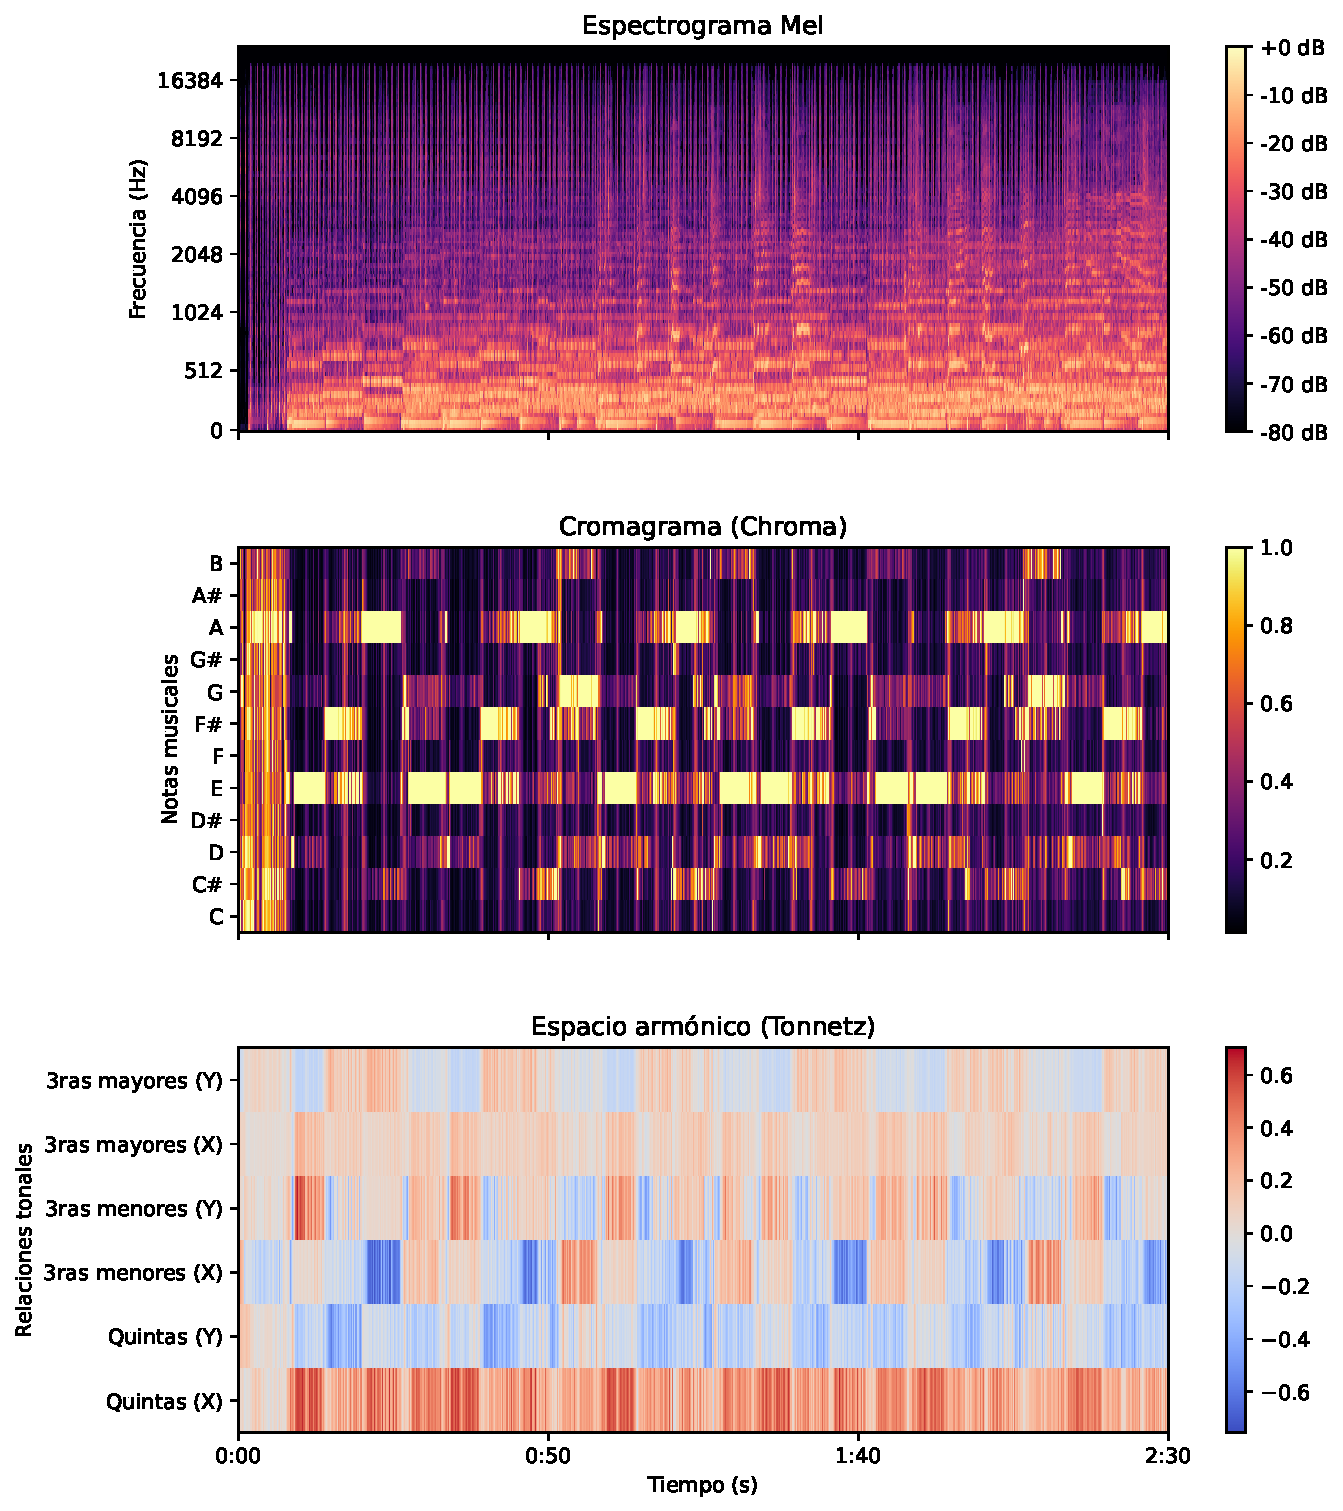
\includegraphics[width=1\textwidth]{./Figures/espectro_croma_tonnetz.pdf}
    \caption[Representaciones visuales del audio]{Representación visual de un espectrograma, un cromagrama y un tonnetz.}
    \label{fig:representaciones_2d}
\end{figure}

Además de las representaciones bidimensionales, las bibliotecas de procesamiento de señales facilitan la extracción de atributos numéricos unidimensionales. En la tabla \ref{tab:atributos_dsp} se presenta un listado que introduce algunas de las características de bajo nivel más representativas en el análisis musical. En la elaboración del trabajo se usaron Librosa y Essentia en este proceso.

Estas transformaciones matemáticas reducen la dimensionalidad del archivo de audio. Sin embargo, carecen de significado semántico. Su función principal, en el contexto de este trabajo, es la de generar las variables predictivas necesarias para entrenar modelos de aprendizaje automático.

El listado completo de las variables de entrada, el análisis de su relevancia y su impacto en el rendimiento de los algoritmos se detalla en el Capítulo 3.

\begin{table}[htpb]
    \centering
    \caption[Atributos representativos]{Listado introductorio de los principales atributos de procesamiento de señales extraídos del audio.}
    \renewcommand{\arraystretch}{1.2}
    \begin{tabular}{p{3.5cm} p{8.5cm}}    
        \toprule
        \textbf{Atributo} & \textbf{Descripción principal} \\
        \midrule
        MFCC & Coeficientes cepstrales que modelan la percepción auditiva humana. \\       
        Centroide espectral & Indica el centro de masa del espectro acústico. Se asocia al brillo del sonido. \\
        Ancho de banda & Mide la dispersión de las frecuencias alrededor del centroide espectral. \\
        Tasa de cruces por cero & Cuantifica la cantidad de cambios de signo en la señal temporal. \\
        Rolloff espectral & Estima la frecuencia por debajo de la que se concentra la mayor parte de la energía. \\
        \bottomrule
    \end{tabular}
    \label{tab:atributos_dsp}
\end{table}

\section{Información semántica del audio}
\label{sec:semantica}

Las representaciones de bajo nivel descritas en la sección 2.2 no siempre son suficientes para capturar conceptos musicales complejos. Es posible mejorar la cobertura de la información musical con el aprendizaje por transferencia. Esta técnica consiste en utilizar modelos previamente entrenados con grandes volúmenes de datos para extraer características semánticas de alto nivel.

Para este fin existen bibliotecas especializadas, como PANNs Inference. Esta herramienta provee acceso a redes neuronales optimizadas para el análisis de eventos sonoros. Dentro de sus opciones, destaca la arquitectura denominada CNN14 \citep{kong2020panns}. Se trata de una red neuronal convolucional, capaz de abstraer patrones del audio y generar embeddings numéricos basados en las clases del conjunto de datos AudioSet. 

Un ejemplo de las probabilidades de detección obtenidas para distintas clases de eventos sonoros a lo largo del tiempo se visualiza en la figura \ref{fig:mapa_semantico}, donde se muestran ventanas consecutivas de 10 segundos de la canción de Radiohead. En este mapa de calor, las áreas más claras indican una mayor probabilidad de activación para cada clase.

El uso de esta arquitectura permite transformar la onda sonora para extraer embeddings y obtener probabilidades asociadas a etiquetas predefinidas, como la presencia de aplausos, instrumentos musicales específicos o habla. Estos datos semánticos enriquecen el conjunto de variables de entrada para la inferencia de algunas de las características musicales que se definieron en el alcance del trabajo.

\newpage
\begin{figure}[!htpb]
    \centering
    
\includegraphics[width=1\textwidth]{mapa_top_clases.pdf}
    \caption[Probabilidades de detección semántica]{Mapa de calor de las características semánticas extraídas mediante la red CNN14.}
    \label{fig:mapa_semantico}
\end{figure}

\section{Modelos de inteligencia artificial utilizados}
\label{sec:modelos}

Una vez obtenidos los descriptores numéricos y semánticos, es necesario aplicar algoritmos de predicción. Para este fin, se utilizaron dos enfoques principales:

\begin{itemize}
    \item Algoritmos LightGBM: se integró la arquitectura LightGBM, basada en el ensamble de árboles de decisión. Esta herramienta destaca por su alta velocidad computacional y eficiencia en tareas generales de predicción.
    \item Redes MLP: los perceptrones multicapa son redes neuronales artificiales con capacidad para modelar relaciones complejas. Permiten, entre otras aplicaciones, predecir múltiples variables continuas de forma simultánea.
\end{itemize}

\section{Despliegue e integración}
\label{sec:despliegue}

La integración del sistema predictivo requirió del despliegue de una interfaz de programación de aplicaciones. Para su construcción se utilizó FastAPI \citep{ramirez2018fastapi} como marco de trabajo. Esta herramienta facilita el desarrollo de servicios web de alto rendimiento basados en Python \citep{python3}.

El alojamiento remoto del producto se apoyó en los servicios de infraestructura de OCI (por su sigla en inglés, Oracle Cloud Infrastructure) \citep{oracle_oci}. Se provisionó una instancia de cómputo virtual en la nube para desplegar la aplicación y ejecutar los modelos predictivos. El uso de esta tecnología garantiza la disponibilidad continua del sistema.

%     \centering
%     \includegraphics[width=0.9\textwidth]{./Figures/diagrama_bloques.pdf}
%     \caption{Diagrama de bloques del sistema en su entorno de despliegue en la nube.}
%     \label{fig:diagrama_despliegue}
% \end{figure}


% \subsection{Uso de mayúscula inicial para los título de secciones}

% Si en el texto se hace alusión a diferentes partes del trabajo referirse a ellas como capítulo, sección o subsección según corresponda. Por ejemplo: ``En el capítulo \ref{Chapter1} se explica tal cosa'', o ``En la sección \ref{sec:ejemplo} se presenta lo que sea'', o ``En la subsección \ref{subsec:ejemplo} se discute otra cosa''.

% Cuando se quiere poner una lista tabulada, se hace así:

% \begin{itemize}
% 	\item Este es el primer elemento de la lista.
% 	\item Este es el segundo elemento de la lista.
% \end{itemize}

% Notar el uso de las mayúsculas y el punto al final de cada elemento.

% Si se desea poner una lista numerada el formato es este:

% \begin{enumerate}
% 	\item Este es el primer elemento de la lista.
% 	\item Este es el segundo elemento de la lista.
% \end{enumerate}

% Notar el uso de las mayúsculas y el punto al final de cada elemento.

% \subsection{Este es el título de una subsección}
% \label{subsec:ejemplo}

% Se recomienda no utilizar \textbf{texto en negritas} en ningún párrafo, ni tampoco texto \underline{subrayado}. En cambio sí se debe utilizar \textit{texto en itálicas} para palabras en un idioma extranjero, al menos la primera vez que aparecen en el texto. En el caso de palabras que estamos inventando se deben utilizar ``comillas'', así como también para citas textuales. Por ejemplo, un \textit{digital filter} es una especie de ``selector'' que permite separar ciertos componentes armónicos en particular.

% La escritura debe ser impersonal. Por ejemplo, no utilizar ``el diseño del firmware lo hice de acuerdo con tal principio'', sino ``el firmware fue diseñado utilizando tal principio''. 

% El trabajo es algo que al momento de escribir la memoria se supone que ya está concluido, entonces todo lo que se refiera a hacer el trabajo se narra en tiempo pasado, porque es algo que ya ocurrió. Por ejemplo, "se diseñó el firmware empleando la técnica de test driven development".

% En cambio, la memoria es algo que está vivo cada vez que el lector la lee. Por eso transcurre siempre en tiempo presente, como por ejemplo:

% ``En el presente capítulo se da una visión global sobre las distintas pruebas realizadas y los resultados obtenidos. Se explica el modo en que fueron llevados a cabo los test unitarios y las pruebas del sistema''.

% Se recomienda no utilizar una sección de glosario sino colocar la descripción de las abreviaturas como parte del mismo cuerpo del texto. Por ejemplo, RTOS (\textit{Real Time Operating System}, Sistema Operativo de Tiempo Real) o en caso de considerarlo apropiado mediante notas a pie de página.

% Si se desea indicar alguna página web utilizar el siguiente formato de referencias bibliográficas, dónde las referencias se detallan en la sección de bibliografía de la memoria, utilizado el formato establecido por IEEE en \citep{IEEE:citation}. Por ejemplo, ``el presente trabajo se basa en la plataforma EDU-CIAA-NXP \citep{CIAA}, la cual...''.

% \subsection{Figuras} 

% Al insertar figuras en la memoria se deben considerar determinadas pautas. Para empezar, usar siempre tipografía claramente legible. Luego, tener claro que \textbf{es incorrecto} escribir por ejemplo esto: ``El diseño elegido es un cuadrado, como se ve en la siguiente figura:''

% \begin{figure}[h]
% \centering
% \includegraphics[scale=.45]{./Figures/cuadradoAzul.png}
% \end{figure}

% La forma correcta de utilizar una figura es con referencias cruzadas, por ejemplo: ``Se eligió utilizar un cuadrado azul para el logo, como puede observarse en la figura \ref{fig:cuadradoAzul}''.

% \begin{figure}[ht]
% 	\centering
% 	\includegraphics[scale=.45]{./Figures/cuadradoAzul.png}
% 	\caption{Ilustración del cuadrado azul que se eligió para el diseño del logo.}
% 	\label{fig:cuadradoAzul}
% \end{figure}

% El texto de las figuras debe estar siempre en español, excepto que se decida reproducir una figura original tomada de alguna referencia. En ese caso la referencia de la cual se tomó la figura debe ser indicada en el epígrafe de la figura e incluida como una nota al pie, como se ilustra en la figura \ref{fig:palabraIngles}.

% \begin{figure}[htpb]
% 	\centering
% 	\includegraphics[scale=.3]{./Figures/word.jpeg}
% 	\caption{Imagen tomada de la página oficial del procesador\protect\footnotemark.}
% 	\label{fig:palabraIngles}
% \end{figure}

% \footnotetext{Imagen tomada de \url{https://goo.gl/images/i7C70w}}

% La figura y el epígrafe deben conformar una unidad cuyo significado principal pueda ser comprendido por el lector sin necesidad de leer el cuerpo central de la memoria. Para eso es necesario que el epígrafe sea todo lo detallado que corresponda y si en la figura se utilizan abreviaturas entonces aclarar su significado en el epígrafe o en la misma figura.



% \begin{figure}[ht]
% 	\centering
% 	\includegraphics[scale=.37]{./Figures/questionMark.png}
% 	\caption{¿Por qué de pronto aparece esta figura?}
% 	\label{fig:questionMark}
% \end{figure}

% Nunca colocar una figura en el documento antes de hacer la primera referencia a ella, como se ilustra con la figura \ref{fig:questionMark}, porque sino el lector no comprenderá por qué de pronto aparece la figura en el documento, lo que distraerá su atención.

% Otra posibilidad es utilizar el entorno \textit{subfigure} para incluir más de una figura, como se puede ver en la figura \ref{fig:three graphs}. Notar que se pueden referenciar también las figuras internas individualmente de esta manera: \ref{fig:1de3}, \ref{fig:2de3} y \ref{fig:3de3}.
 
% \begin{figure}[!htpb]
%      \centering
%      \begin{subfigure}[b]{0.3\textwidth}
%          \centering
%          \includegraphics[width=.65\textwidth]{./Figures/questionMark}
%          \caption{Un caption.}
%          \label{fig:1de3}
%      \end{subfigure}
%      \hfill
%      \begin{subfigure}[b]{0.3\textwidth}
%          \centering
%          \includegraphics[width=.65\textwidth]{./Figures/questionMark}
%          \caption{Otro.}
%          \label{fig:2de3}
%      \end{subfigure}
%      \hfill
%      \begin{subfigure}[b]{0.3\textwidth}
%          \centering
%          \includegraphics[width=.65\textwidth]{./Figures/questionMark}
%          \caption{Y otro más.}
%          \label{fig:3de3}
%      \end{subfigure}
%         \caption{Tres gráficos simples.}
%         \label{fig:three graphs}
% \end{figure}

% El código para generar las imágenes se encuentra disponible para su reutilización en el archivo \file{Chapter2.tex}.

% \subsection{Tablas}

% Para las tablas utilizar el mismo formato que para las figuras, sólo que el epígrafe se debe colocar arriba de la tabla, como se ilustra en la tabla \ref{tab:peces}. Observar que sólo algunas filas van con líneas visibles y notar el uso de las negritas para los encabezados.  La referencia se logra utilizando el comando \verb|\ref{<label>}| donde label debe estar definida dentro del entorno de la tabla.

% \begin{verbatim}
% \begin{table}[h]
% 	\centering
% 	\caption[caption corto]{caption largo más descriptivo}
% 	\begin{tabular}{l c c}    
% 		\toprule
% 		\textbf{Especie}     & \textbf{Tamaño} & \textbf{Valor}\\
% 		\midrule
% 		Amphiprion Ocellaris & 10 cm           & \$ 6.000 \\		
% 		Hepatus Blue Tang    & 15 cm           & \$ 7.000 \\
% 		Zebrasoma Xanthurus  & 12 cm           & \$ 6.800 \\
% 		\bottomrule
% 		\hline
% 	\end{tabular}
% 	\label{tab:peces}
% \end{table}
% \end{verbatim}


% \begin{table}[h]
% 	\centering
% 	\caption[caption corto]{caption largo más descriptivo.}
% 	\begin{tabular}{l c c}    
% 		\toprule
% 		\textbf{Especie} 	 & \textbf{Tamaño} 		& \textbf{Valor}  \\
% 		\midrule
% 		Amphiprion Ocellaris & 10 cm 				& \$ 6.000 \\		
% 		Hepatus Blue Tang	 & 15 cm				& \$ 7.000 \\
% 		Zebrasoma Xanthurus	 & 12 cm				& \$ 6.800 \\
% 		\bottomrule
% 		\hline
% 	\end{tabular}
% 	\label{tab:peces}
% \end{table}

% En cada capítulo se debe reiniciar el número de conteo de las figuras y las tablas, por ejemplo, figura 2.1 o tabla 2.1, pero no se debe reiniciar el conteo en cada sección. Por suerte la plantilla se encarga de esto por nosotros.

% \subsection{Ecuaciones}
% \label{sec:Ecuaciones}

% Al insertar ecuaciones en la memoria dentro de un entorno \textit{equation}, éstas se numeran en forma automática  y se pueden referir al igual que como se hace con las figuras y tablas, por ejemplo ver la ecuación \ref{eq:metric}.

% \begin{equation}
% 	\label{eq:metric}
% 	ds^2 = c^2 dt^2 \left( \frac{d\sigma^2}{1-k\sigma^2} + \sigma^2\left[ d\theta^2 + \sin^2\theta d\phi^2 \right] \right)
% \end{equation}
                                                        
% Para generar la ecuación \ref{eq:metric} se utilizó el siguiente código:

% \begin{verbatim}
% \begin{equation}
% 	\label{eq:metric}
% 	ds^2 = c^2 dt^2 \left( \frac{d\sigma^2}{1-k\sigma^2} + 
% 	\sigma^2\left[ d\theta^2 + 
% 	\sin^2\theta d\phi^2 \right] \right)
% \end{equation}
% \end{verbatim}
 
% 	\chapter{Diseño e implementación} % Main chapter title

\label{Chapter3} % Change X to a consecutive number; for referencing this chapter elsewhere, use \ref{ChapterX}

% Todos los capítulos deben comenzar con un breve párrafo introductorio que indique cuál es el contenido que se encontrará al leerlo.  La redacción sobre el contenido de la memoria debe hacerse en presente y todo lo referido al proyecto en pasado, siempre de modo impersonal.

\definecolor{mygreen}{rgb}{0,0.6,0}
\definecolor{mygray}{rgb}{0.5,0.5,0.5}
\definecolor{mymauve}{rgb}{0.58,0,0.82}

%%%%%%%%%%%%%%%%%%%%%%%%%%%%%%%%%%%%%%%%%%%%%%%%%%%%%%%%%%%%%%%%%%%%%%%%%%%%%
% parámetros para configurar el formato del código en los entornos lstlisting
%%%%%%%%%%%%%%%%%%%%%%%%%%%%%%%%%%%%%%%%%%%%%%%%%%%%%%%%%%%%%%%%%%%%%%%%%%%%%
\lstset{ %
  backgroundcolor=\color{white},   % choose the background color; you must add \usepackage{color} or \usepackage{xcolor}
  basicstyle=\footnotesize,        % the size of the fonts that are used for the code
  breakatwhitespace=false,         % sets if automatic breaks should only happen at whitespace
  breaklines=true,                 % sets automatic line breaking
  captionpos=b,                    % sets the caption-position to bottom
  commentstyle=\color{mygreen},    % comment style
  deletekeywords={...},            % if you want to delete keywords from the given language
  %escapeinside={\%*}{*)},          % if you want to add LaTeX within your code
  %extendedchars=true,              % lets you use non-ASCII characters; for 8-bits encodings only, does not work with UTF-8
  %frame=single,	                % adds a frame around the code
  keepspaces=true,                 % keeps spaces in text, useful for keeping indentation of code (possibly needs columns=flexible)
  keywordstyle=\color{blue},       % keyword style
  language=Python,                % the language of the code
  %otherkeywords={*,...},           % if you want to add more keywords to the set
  numbers=left,                    % where to put the line-numbers; possible values are (none, left, right)
  numbersep=5pt,                   % how far the line-numbers are from the code
  numberstyle=\tiny\color{mygray}, % the style that is used for the line-numbers
  rulecolor=\color{black},         % if not set, the frame-color may be changed on line-breaks within not-black text (e.g. comments (green here))
  showspaces=false,                % show spaces everywhere adding particular underscores; it overrides 'showstringspaces'
  showstringspaces=false,          % underline spaces within strings only
  showtabs=false,                  % show tabs within strings adding particular underscores
  stepnumber=1,                    % the step between two line-numbers. If it's 1, each line will be numbered
  stringstyle=\color{mymauve},     % string literal style
  tabsize=2,	                   % sets default tabsize to 2 spaces
  title=\lstname,                  % show the filename of files included with \lstinputlisting; also try caption instead of title
  morecomment=[s]{/*}{*/}
}


Este capítulo detalla el diseño y la implementación del sistema predictivo. Se analizan los conjuntos de datos utilizados, la extracción de atributos del audio y el tratamiento de datos según las distribuciones de las variables objetivo. Asimismo, se describen las técnicas de reducción y selección de variables, el proceso de optimización de los modelos y los resultados de la iteración productiva. Finalmente, se presenta la arquitectura desarrollada para el despliegue y la integración del sistema en un entorno operativo.

%----------------------------------------------------------------------------------------
%	SECTION 1
%----------------------------------------------------------------------------------------
\section{Conjuntos de datos}
\label{sec:conjuntos_datos}
% Aquí se describirá la extracción de datos del audio.

\subsection{Análisis de conjuntos de datos públicos}

La definición de la estrategia para la extracción de atributos se fundamenta en una revisión de conjuntos de datos públicos estandarizados en el ámbito MIR. 
El objetivo fue entender cómo repositorios de referencia, como FMA y Million Song Dataset, representan y estructuran los datos musicales, para decidir su viabilidad en el contexto de aplicación de este trabajo. 

\subsubsection{GTZAN}
Este conjunto de datos se considera el equivalente al MNIST \cite{lecun1998gradient} para el análisis de audio \cite{sturm2014state}, dada su adopción histórica como estándar de evaluación en tareas de clasificación de géneros musicales.
\begin{itemize}
    \item Variables predictivas principales: tempo, representaciones chroma, amplitud media cuadrática (RMS), descriptores espectrales y coeficientes MFCC.
    \item Estructura: 1~000 archivos de audio en crudo limitados a 30 segundos, acompañados de metadatos tabulares e imágenes de espectrogramas de Mel en su versión distribuida mediante Kaggle \citep{gtzan_kaggle}. 
    Todas estas representaciones fueron extraídas utilizando la biblioteca Librosa. Las tablas contienen los atributos calculados sobre la pista completa y también sobre divisiones de 3 segundos para incrementar el volumen de datos de entrenamiento. En ambos escenarios se aplica una reducción de dimensionalidad temporal: las variables se calculan inicialmente sobre micro-ventanas de milisegundos y luego se colapsan a valores estáticos mediante estadísticos de agregación, como la media y la varianza.
    \item Variables objetivo principales en Plusyc: se podría relacionar con \textit{suggested genres}. 
    \item Desventajas: provee segmentos cortos de audio, lo que limita la representatividad de la información musical a nivel de canción; y solo abarca 10 géneros musicales, mientras que Plusyc trabaja con más de 500.
\end{itemize}

\subsubsection{FMA estándar}
Se analiza la versión estándar de FMA, diseñada para superar las limitaciones de tamaño y acceso a las colecciones completa y mediana.
\begin{itemize}
    \item Variables predictivas principales: representaciones chroma, Transformada de Q Constante (CQT), tonnetz, MFCC, RMS, descriptores espectrales y tasa de cruces por cero (ZCR).
    \item Estructura: ofrece recortes de audio de 30 segundos para sus subconjuntos estándar, acompañados de matrices de atributos precomputados distribuidos en formato tabular (CSV). Los atributos fueron extraídos utilizando Librosa y posteriormente colapsados mediante estadísticos de agregación, como la media, desviación estándar, asimetría y curtosis, para obtener valores estáticos por pista.
    \item Metadatos contextuales: información tabular adicional que incluye álbum, artista, popularidad, fechas de lanzamiento y ubicación geográfica.
    \item Variables objetivo principales: géneros musicales estructurados en una taxonomía jerárquica de clases y para un subconjunto de aproximadamente 13~000 pistas, proporciona atributos como \textit{danceability, energy, valence, speechiness} y \textit{liveness}.
    \item Desventajas: el análisis está restringido a segmentos de 30 segundos en la versión estándar. Las versiones media y completa exceden las capacidades de procesamiento de la infraestructura actual de la empresa. Además, la incertidumbre sobre las versiones exactas de Librosa utilizadas originalmente dificulta la replicabilidad técnica sobre canciones nuevas. Finalmente, la información etiquetada de 13~000 pistas es mucho menor que la de más de 60~000 de Plusyc.
\end{itemize}

\subsubsection{Million Song Dataset (MSD)}
Desarrollado por la Universidad de Columbia y The Echo Nest \cite{bertin2011million}, este conjunto escaló la investigación de información musical a nivel industrial.
\begin{itemize}
    \item Variables predictivas principales: representaciones de tono (chroma y pitch) y descriptores de timbre, ambos calculados a nivel de segmento.
    \item Estructura: colección de metadatos y descriptores precomputados empaquetados en archivos HDF5.
    \item Método de extracción: a diferencia de la segmentación por ventanas fijas, el MSD utiliza una división adaptativa basada en eventos. Esto fragmenta la canción en segmentos de duración variable. Para cada uno de estos segmentos, se calculan coeficientes de tono y timbre, y se genera una matriz de atributos alineada con la estructura temporal de la pista.
    \item Variables objetivo principales: proporciona atributos musicales fundamentales como \textit{tempo, loudness, key} y \textit{mode}.
    \item Desventajas: los descriptores se generaron con algoritmos propietarios de The Echo Nest, lo que complica procesar la segmentación por eventos en canciones nuevas de forma idéntica para realizar el proceso de inferencia.
\end{itemize}

\subsubsection{AudioSet}
Este conjunto masivo establece un estándar para la clasificación de eventos sonoros generales
\begin{itemize}
    \item Estructura: conjunto de identificadores de videos de YouTube y marcas de tiempo que referencian segmentos de 10 segundos, anotados bajo una ontología de 527 clases.
    \item Variables predictivas principales: el corpus original no extrae descriptores tradicionales. Su distribución oficial provee embeddings precomputados mediante el modelo VGGish \cite{hershey2017cnn}, que sirven como entrada rápida para entrenar clasificadores de terceros sin necesidad de descargar el audio original.
    \item Variables objetivo principales: etiquetas multiclase que identifican la presencia de instrumentos musicales, como tipos de voces (habla, canto) y ambientes acústicos.
    \item Desventajas: el enfoque en sonidos generales limita su precisión para los atributos musicales.
\end{itemize}

% En la tabla \ref{tab:variables_datasets} se presentan algunas de las variables predictivas más relevantes de cada conjunto de datos.

Todos estos conjuntos de datos presentan varias limitaciones frente a la solución propuesta: algunos restringen el análisis a segmentos cortos de audio, mientras que otros requieren tamaños de almacenamiento excesivamente pesados o estructuras de datos difíciles de replicar durante el proceso de inferencia y dependientes de las versiones de las bibliotecas de extracción.

Por otro lado, estas restricciones motivaron que el proceso de extracción se ejecute directamente sobre el catálogo privado para eliminar las limitaciones, y su revisión permitió sentar las bases para determinar cuáles son las variables predictivas en la música, cómo se segmentan las canciones, cómo se reduce la dimensionalidad y para hacer los primeros experimentos predictivos de las variables objetivo requeridas.

Cabe mencionar que, a pesar de que en algunas de las fuentes de datos públicas se incluye información del contexto como la región del artista, el año de lanzamiento, el álbum o las letras, en esta solución se trabaja exclusivamente con información musical que se extrae del audio. 

\subsection{Reducción de dimensionalidad mediante estadísticas}

En el ámbito del procesamiento de señales, la información de un archivo de audio se representa como una serie de tiempo multivariada: una secuencia de puntos de datos \cite{muller2015fundamentals}, en este caso, descriptores numéricos y semánticos, indexados y ordenados cronológicamente.

La estrategia adoptada se inspiró en los conjuntos de datos de referencia, donde la señal se divide en ventanas temporales y la información de cada ventana se colapsa en valores estáticos. Esto permite reducir estas secuencias a un vector por cada canción, buscando optimizar el uso de la memoria y los tiempos de procesamiento.
Esta transformación de la señal de secuencias de números a un vector de estadísticos ocurre de la siguiente manera:

\begin{itemize}
    \item Segmentación temporal: se estableció una ventana de análisis de 10 segundos continuos. Esta decisión se fundamenta en la arquitectura de la red neuronal CNN14, entrenada sobre el conjunto de datos AudioSet, cuyos segmentos originales son de 10 segundos.
    \item Extracción de variables predictivas: para cada segmento de 10 segundos de la canción, el algoritmo usa Librosa y Essentia para extraer el conjunto de variables predictivas principales que proveen las fuentes de datos públicos. También se extrae información global de la canción y algunas de las variables predictivas escalares se calculan de forma global y también de forma segmentada y agregada.
    \item Extracción de embeddings y probabilidades: para esos segmentos de 10 segundos, el algoritmo también extrae un vector de embeddings y las probabilidades de activación para 173 clases de eventos musicales provistas por PANNs inference.
    \item Agrupación estadística: dado que una canción estándar produce una cantidad variable de segmentos de 10 segundos, se aplicó una técnica de colapso estadístico a lo largo del eje temporal, diferenciando el tratamiento según el tipo de variable:
    \begin{itemize}
        \item Para las variables predictivas (DSP), se calcularon siete estadísticos por pista: media, desviación estándar, asimetría, curtosis, y los percentiles 10 (cerca del mínimo), 50 (mediana) y 90 (cerca del máximo para evitar ruido).
        \item Para los embeddings y las probabilidades semánticas de las 173 clases seleccionadas de PANNs, se calcularon cuatro medidas: media, valor máximo, desviación estándar y el percentil 90.
    \end{itemize}
\end{itemize}

Este enfoque matemático permite comprimir el volumen masivo de información de una serie de tiempo en un único vector unidimensional por canción.

Algunos experimentos preliminares sirvieron para validar que esta representación permitía capturar la información esencial de la canción de manera eficiente y compacta.
El algoritmo de extracción, es el resultado de múltiples pruebas con distintas configuraciones de variables, estadísticos y métodos de segmentación. Algunos de los experimentos que no resultaron exitosos comprenden:
pruebas con solo variables predictivas sin embeddings, demuestran que no es posible capturar eventos como el público en vivo o el habla en los primeros intentos de inferencia de \textit{liveness} y \textit{speechiness}. Las pruebas con embeddings pero sin variables predictivas en general no proporcionan la información de \textit{key}, \textit{tempo}, \textit{loudness}, \textit{mood} o \textit{genres}.
Pruebas con distintas ventanas resultaron ser ineficientes en el proceso de extracción de más de 60~000 canciones. Pruebas aplicando todos los estadísticos resultaron en un espacio de variables que consume mucho espacio de almacenamiento y con alta correlación.

\subsection{Conformación del espacio de variables masivo}
% Tras validar la superioridad de la arquitectura mixta, se ejecutó el proceso de extracción sobre el catálogo completo. El procesamiento computacional requirió más de una semana de ejecución ininterrumpida para procesar las canciones completas.

% El algoritmo de extracción definitivo combinó las funciones de Librosa y Essentia con la inferencia de la red neuronal CNN14. El resultado fue un conjunto de datos masivo compuesto por más de 9000 variables predictivas independientes por cada registro de audio. Este extenso espacio de características garantiza la disponibilidad de toda la información acústica y semántica posible para la etapa de experimentación. El alto costo computacional de la extracción justifica esta estrategia de recopilación exhaustiva, eliminando la necesidad de reprocesar el audio y trasladando el desafío técnico hacia la selección rigurosa de las variables más relevantes durante la etapa de modelado, proceso que se detalla en la sección \ref{sec:seleccion_variables} %.


\section{Ejecución de tareas sobre el conjunto de datos}
\label{sec:ejecucion_tareas}
% Aquí se detallarán las distribuciones de las variables objetivo, dificultades encontradas y estrategias de muestreo.


\section{Selección de variables de entrada}
\label{sec:seleccion_variables}
% Aquí se describirán las técnicas de selección y reducción para una arquitectura mixta.


\section{Modelado y optimización}
\label{sec:modelado_optimizacion}
% Aquí se abordará el proceso de modelado y la búsqueda de hiperparámetros.


\section{Iteración productiva}
\label{sec:iteracion_productiva}
% Aquí se presentarán los resultados generales de la iteración.


\section{Arquitectura de despliegue e integración}
\label{sec:arquitectura_despliegue}
% Aquí se documentará la arquitectura para el despliegue e integración en un ambiente productivo.

% La idea de esta sección es resaltar los problemas encontrados, los criterios utilizados y la justificación de las decisiones que se hayan tomado.
% Se puede agregar código o pseudocódigo dentro de un entorno lstlisting con el siguiente código:




\begin{verbatim}
\begin{lstlisting}[caption= "un epígrafe descriptivo"]
	las líneas de código irían aquí...
\end{lstlisting}
\end{verbatim}

A modo de ejemplo, se muestra el fragmento de código \ref{cod:vControl}:

\begin{lstlisting}[label=cod:vControl,caption=Pseudocódigo del lazo principal de control.]  % Start your code-block

#define MAX_SENSOR_NUMBER 3
#define MAX_ALARM_NUMBER  6
#define MAX_ACTUATOR_NUMBER 6

uint32_t sensorValue[MAX_SENSOR_NUMBER];		
FunctionalState alarmControl[MAX_ALARM_NUMBER];	//ENABLE or DISABLE
state_t alarmState[MAX_ALARM_NUMBER];						//ON or OFF
state_t actuatorState[MAX_ACTUATOR_NUMBER];			//ON or OFF

void vControl() {

	initGlobalVariables();
	
	period = 500 ms;
		
	while(1) {

		ticks = xTaskGetTickCount();
		
		updateSensors();
		
		updateAlarms();
		
		controlActuators();
		
		vTaskDelayUntil(&ticks, period);
	}
}
\end{lstlisting}




% 	% Chapter Template

% todo en la parte de datasets se me sugirió mover aquí esto...
% Algunos de los experimentos que no resultaron exitosos comprenden:
% pruebas con solo variables predictivas sin embeddings, demuestran que no es posible capturar eventos como el público en vivo o el habla en los primeros intentos de inferencia de \textit{liveness} y \textit{speechiness}. Las pruebas con embeddings pero sin variables predictivas en general no proporcionan la información de \textit{key}, \textit{tempo}, \textit{loudness}, \textit{mood} o \textit{genres}.
% Pruebas con distintas ventanas resultaron ser ineficientes en el proceso de extracción de más de 60~000 canciones. Pruebas aplicando todos los estadísticos resultaron en un espacio de variables que consume mucho espacio de almacenamiento y con alta correlación.

\chapter{Ensayos y resultados} % Main chapter title

\label{Chapter4} % Change X to a consecutive number; for referencing this chapter elsewhere, use \ref{ChapterX}
Todos los capítulos deben comenzar con un breve párrafo introductorio que indique cuál es el contenido que se encontrará al leerlo.  La redacción sobre el contenido de la memoria debe hacerse en presente y todo lo referido al proyecto en pasado, siempre de modo impersonal.

%todo Dada la complejidad de objetivos como los géneros musicales, 197 clases resultantes, se priorizó el análisis de la precisión \textit{Top-K} para capturar la pluralidad semántica de la música
%----------------------------------------------------------------------------------------
%	SECTION 1
%----------------------------------------------------------------------------------------

\section{Pruebas funcionales del hardware}
\label{sec:pruebasHW}

La idea de esta sección es explicar cómo se hicieron los ensayos, qué resultados se obtuvieron y analizarlos.
 
% 	% Chapter Template

\chapter{Conclusiones} % Main chapter title

Este capítulo presenta un resumen de los logros y las dificultades para llegar al estado actual de la solución y sugiere una serie de siguientes pasos para la evolución del sistema.

\label{Chapter5} % Change X to a consecutive number; for referencing this chapter elsewhere, use \ref{ChapterX}

\section{Conclusiones generales}

En este trabajo se propuso diseñar e implementar un sistema capaz de predecir características musicales a partir de audio de canciones. El objetivo principal fue automatizar
un proceso tradicionalmente manual y laborioso de clasificación musical y reducir la dependencia de servicios de tercecros para evitar costos recurrentes.
El trabajo está en producción, clasifica las canciones que ingresan al sistema, es funcional en el contexto de una empresa en crecimiento. 

En relación a los objetivos específicos, se puede concluir que:

%----------------------------------------------------------------------------------------

%----------------------------------------------------------------------------------------
%	SECTION 1
%----------------------------------------------------------------------------------------

\begin{itemize}
\item Se cumplieron los requerimientos técnicos al lograr la caracterización de las variables solicitadas a partir de los datos de Plusyc.
\item La extracción de variables acústicas DSP sirvió para las predicciones, y la inclusión de embeddings y probabilidades de PANNs fue lo que permitió resolver las variables semánticas complejas. Sin esto último, no se habría completado el trabajo.
\item Se aplicaron acciones para mitigar problemas en los datos. Fue necesario aplicar técnicas de preprocesamiento; se cortó el histórico en una fecha específica para aislar un cambio en la distribución de los datos.
\item Se entrenaron modelos de aprendizaje automático para predecir las características musicales y la evaluación de las métricas de rendimiento dan resultados productivos, acorde al análisis y diseño realizados.
\item La decisión de usar bibliotecas como Librosa y PANNs inference y modelos como redes MLP y ensambles de árboles, permitió no depender de licencias ni pagar costos por consultas a modelos de terceros, también facilitó el trabajo al no requerir de arquitecturas complejas.
\item En específico, la clasificación de estados de ánimo y géneros sugiere que la ambigüedad humana al etiquetar afecta el aprendizaje. Estos resultados indican que el equipo de curaduría necesita estandarizar los criterios para la ingesta manual de datos.
\item Para la detección de público en vivo y habla en canciones, se requirió de limpieza de ruido por falsas etiquetas apoyada en un modelo preentrenado con el conjunto de datos AudioSet, creado para la generación automática de subtítulos como [Aplausos] o [Rapping].
\item Completar el trabajo tomó más tiempo del planificado en el cronograma original. Hubo una subestimación del esfuerzo, dado que la cantidad de modelos y el proceso de aprendizaje requirieron más iteraciones de las previstas.

\end{itemize}

\section{Próximos pasos}

Los diseños actuales quedan disponibles y se pueden usar para iteraciones futuras. Algunos aspectos que se podrían mejorar o explorar son:

\begin{itemize}
\item El uso de las inferencias de PANNs y la exploración de otros modelos preentrenados, para mejorar la limpieza de algunos datos y corregir audios mal etiquetados.
Como ejemplos, el \textit{speechiness}, \textit{liveness} y la predicción de \textit{instrumentalness}: el modelo actual logra diferenciar una canción instrumental de una que no lo es, pero los valores en el medio no son claros. 
Se sugiere revisar puntualmente, ya que presenta ruido en los valores intermedios por falta de definiciones claras.
\item También se sugiere iterar sobre el \textit{tempo} para buscar una solución más robusta que el algoritmo de DSP.
\item Se propone empezar a usar el estado de ánimo secundario como filtro en Plusyc para mejorar la precisión de las recomendaciones musicales.
\item El sistema se puede ajustar para el despliegue bajo el modelo de software como servicio y así permitir ofrecer el servicio al público interesado.
\item El equipo de curadores sigue clasificando música. Se contempla automatizar un reentrenamiento periódico para que el sistema aprenda nuevos géneros cada vez que una clase alcance un mínimo de 100 muestras, con el uso de tecnologías como Airflow y MLflow para optimizar estos procesos, hoy manuales.
\item Se podría evaluar a futuro el uso de arquitecturas basadas en transformadores, si se cuenta con mayor capacidad de cómputo, para mejorar la clasificación de clases densas. 
También, complementar el sistema con modelos de aprendizaje profundo enfocados exclusivamente en música.
\end{itemize}
%----------------------------------------------------------------------------------------

%   SECTION 2

%----------------------------------------------------------------------------------------

% \section{Próximos pasos}



% Acá se indica cómo se podría continuar el trabajo más adelante.



% \section{Conclusiones generales}

% % Este capítulo resume los hallazgos del proyecto y establece la hoja de ruta para su evolución en Plusyc.

% \begin{itemize}
% \item Se cumplió la totalidad de los requerimientos técnicos al lograr la caracterización de las variables acústicas solicitadas.
% \item La ejecución tomó más tiempo del planificado en el cronograma original. Hubo una subestimación del esfuerzo, ya que la cantidad de modelos obligó a iterar más de lo previsto para encontrar resultados aceptables.
% \item Se aplicaron acciones para mitigar problemas en los datos. Se cortó el histórico en enero de 2026 para aislar un cambio en la distribución de los registros. Además, se usó submuestreo y limpieza con modelos preentrenados para compensar el desbalance en clases como liveness y speechiness.
% \item La extracción de variables acústicas tradicionales sirvió como base, pero la inclusión de embeddings y probabilidades de PANNs fue lo que permitió resolver las variables semánticas complejas. Sin esto último, no se habría completado el trabajo.
% \item La clasificación de estados de ánimo y géneros demostró que la ambigüedad humana al etiquetar afecta el aprendizaje. Estos resultados indican que el equipo de curaduría necesita estandarizar los criterios para la ingesta manual de datos.
% \item Se optó por usar PyTorch y PANNs para no depender de licencias ni pagar costos por consultas a modelos de terceros. El sistema se desplegó bajo el modelo de software como servicio para facilitar un procesamiento escalable y asíncrono.
% \end{itemize}

% \section{Próximos pasos}

% % Acá se indica cómo se podría continuar el trabajo más adelante.

% \begin{itemize}
% \item Los modelos actuales quedan como base para iteraciones futuras. Se debe revisar puntualmente instrumentalness, ya que presenta mucho ruido por falta de definiciones claras en los valores intermedios.
% \item Se deja como trabajo pendiente usar las inferencias de PANNs para automatizar la limpieza de datos en el histórico y corregir audios mal etiquetados.
% \item El equipo de curadores sigue clasificando música. Se contempla automatizar un reentrenamiento periódico para que el sistema aprenda nuevos géneros cada vez que una clase alcance un mínimo de 100 muestras.
% \item Se propone empezar a usar el estado de ánimo secundario como filtro en Plusyc para mejorar la precisión de las recomendaciones musicales.
% \item Se sugiere evaluar a futuro el uso de arquitecturas basadas en transformadores para audios, si se cuenta con mayor capacidad de cómputo, para buscar mejoras en la clasificación de clases densas como los géneros.
% \end{itemize} 
% \end{verbatim}

% Los apéndices también deben escribirse en archivos .tex separados, que se deben ubicar dentro de la carpeta \emph{Appendices}. Los apéndices vienen comentados por defecto con el caracter \code{\%} y para incluirlos simplemente se debe eliminar dicho caracter.

% Finalmente, se encuentra el código para incluir la bibliografía en el documento final.  Este código tampoco debe modificarse. La metodología para trabajar las referencias bibliográficas se desarrolla en la sección \ref{sec:biblio}.
%----------------------------------------------------------------------------------------

% \section{Bibliografía}
% \label{sec:biblio}

% Las opciones de formato de la bibliografía se controlan a través del paquete de latex \option{biblatex} que se incluye en la memoria en el archivo memoria.tex.  Estas opciones determinan cómo se generan las citas bibliográficas en el cuerpo del documento y cómo se genera la bibliografía al final de la memoria.

% En el preámbulo se puede encontrar el código que incluye el paquete biblatex, que no requiere ninguna modificación del usuario de la plantilla, y que contiene las siguientes opciones:

% \begin{lstlisting}
% \usepackage[backend=bibtex,
% 	natbib=true, 
% 	style=numeric, 
% 	sorting=none]
% {biblatex}
% \end{lstlisting}

% En el archivo \file{reference.bib} se encuentran las referencias bibliográficas que se pueden citar en el documento.  Para incorporar una nueva cita al documento lo primero es agregarla en este archivo con todos los campos necesario.  Todas las entradas bibliográficas comienzan con $@$ y una palabra que define el formato de la entrada.  Para cada formato existen campos obligatorios que deben completarse. No importa el orden en que las entradas estén definidas en el archivo .bib.  Tampoco es importante el orden en que estén definidos los campos de una entrada bibliográfica. A continuación se muestran algunos ejemplos:

% \begin{lstlisting}
% @ARTICLE{ARTICLE:1,
%     AUTHOR="John Doe",
%     TITLE="Title",
%     JOURNAL="Journal",
%     YEAR="2017",
% }
% \end{lstlisting}


% \begin{lstlisting}
% @BOOK{BOOK:1,
%     AUTHOR="John Doe",
%     TITLE="The Book without Title",
%     PUBLISHER="Dummy Publisher",
%     YEAR="2100",
% }
% \end{lstlisting}


% \begin{lstlisting}
% @INBOOK{BOOK:2,
%     AUTHOR="John Doe",
%     TITLE="The Book without Title",
%     PUBLISHER="Dummy Publisher",
%     YEAR="2100",
%     PAGES="100-200",
% }
% \end{lstlisting}


% \begin{lstlisting}
% @MISC{WEBSITE:1,
%     HOWPUBLISHED = "\url{http://example.com}",
%     AUTHOR = "Intel",
%     TITLE = "Example Website",
%     MONTH = "12",
%     YEAR = "1988",
%     URLDATE = {2012-11-26}
% }
% \end{lstlisting}

% Se debe notar que los nombres \emph{ARTICLE:1}, \emph{BOOK:1}, \emph{BOOK:2} y \emph{WEBSITE:1} son nombres de fantasía que le sirve al autor del documento para identificar la entrada. En este sentido, se podrían reemplazar por cualquier otro nombre.  Tampoco es necesario poner : seguido de un número, en los ejemplos sólo se incluye como un posible estilo para identificar las entradas.

% La entradas se citan en el documento con el comando: 

% \begin{verbatim}
% \citep{nombre_de_la_entrada}
% \end{verbatim}

% Y cuando se usan, se muestran así: \citep{ARTICLE:1}, \citep{BOOK:1}, \citep{BOOK:2}, \citep{WEBSITE:1}.  Notar cómo se conforma la sección Bibliografía al final del documento.

% Finalmente y como se mencionó en la subsección \ref{subsec:configurando}, para actualizar las referencias bibliográficas tanto en la sección bibliografía como las citas en el cuerpo del documento, se deben ejecutar las herramientas de compilación PDFLaTeX, BibTeX, PDFLaTeX, PDFLaTeX, en ese orden.  Este procedimiento debería resolver cualquier mensaje "Citation xxxxx on page x undefined".

\chapter{Introducción específica} % Main chapter title

\label{Chapter2}

%----------------------------------------------------------------------------------------
%	SECTION 1
%----------------------------------------------------------------------------------------
Este capítulo introduce las herramientas de terceros y las tecnologías necesarias para el desarrollo del sistema. Se describe la fuente de datos principal, las técnicas para extraer representaciones numéricas del audio, los modelos predictivos y las tecnologías utilizadas para el despliegue.

\section{Fuentes de datos de canciones}
\label{sec:datos}

Para el entrenamiento de los modelos predictivos se utilizó la colección privada de canciones de la empresa. Esta fuente de datos cuenta con más de 60~000 archivos de audio de canciones completas.

Se seleccionó este conjunto de datos por la disponibilidad en el acceso a la información y por su representatividad en ambientes comerciales reales. Por el contrario, otros conjuntos de datos públicos musicales, como GTZAN \citep{GTZAN} y los subconjuntos estándar de FMA \citep{FMA}, ofrecen fragmentos limitados a 10 o 30 segundos de audio. El uso de pistas incompletas restringe la disponibilidad de la información musical. Realizar predicciones sobre el audio total resulta más preciso, ya que evita la pérdida de los eventos musicales que ocurren antes o después de una sola ventana. Además, estas alternativas carecen parcialmente de las variables objetivo requeridas en el alcance del trabajo.

El acceso a los archivos de audio de canciones completas garantiza la preservación de la estructura musical, evita la pérdida de información y flexibiliza la extracción de representaciones matemáticas mediante el uso de bibliotecas y modelos preentrenados.

El análisis comparativo de las fuentes de datos, las representaciones estadísticas de las canciones y los criterios de selección de variables predictivas se detallan en el Capítulo 3.
% TODO: Cambiar "Capítulo 3" por las referencias cruzadas (\ref{}) de las secciones exactas una vez que se termine de escribir el Capítulo 3.

\section{Representaciones numéricas de la música}
\label{sec:dsp}

Una canción se traduce a un formato numérico para su procesamiento computacional. El procesamiento digital de señales (DSP) transforma la onda sonora en arreglos matemáticos de una o dos dimensiones. 
Entre las representaciones bidimensionales más destacadas se encuentran el espectrograma, el cromagrama y el espacio armónico o tonnetz. El espectrograma refleja la variación de las frecuencias a lo largo del tiempo. Por su parte, el cromagrama captura la energía asociada a las doce clases de notas musicales. Finalmente, el tonnetz modela las relaciones tonales y armónicas de la pista. A modo de ejemplo, en la figura \ref{fig:representaciones_2d} se ilustran estas tres transformaciones aplicadas a un fragmento de la canción ``Weird Fishes/Arpeggi'' de la banda Radiohead. En estos gráficos, el eje horizontal representa el tiempo, mientras que la intensidad del color indica la magnitud de la energía para las distintas frecuencias, notas musicales o relaciones tonales correspondientes a cada eje vertical.

\begin{figure}[htpb]
    \centering
    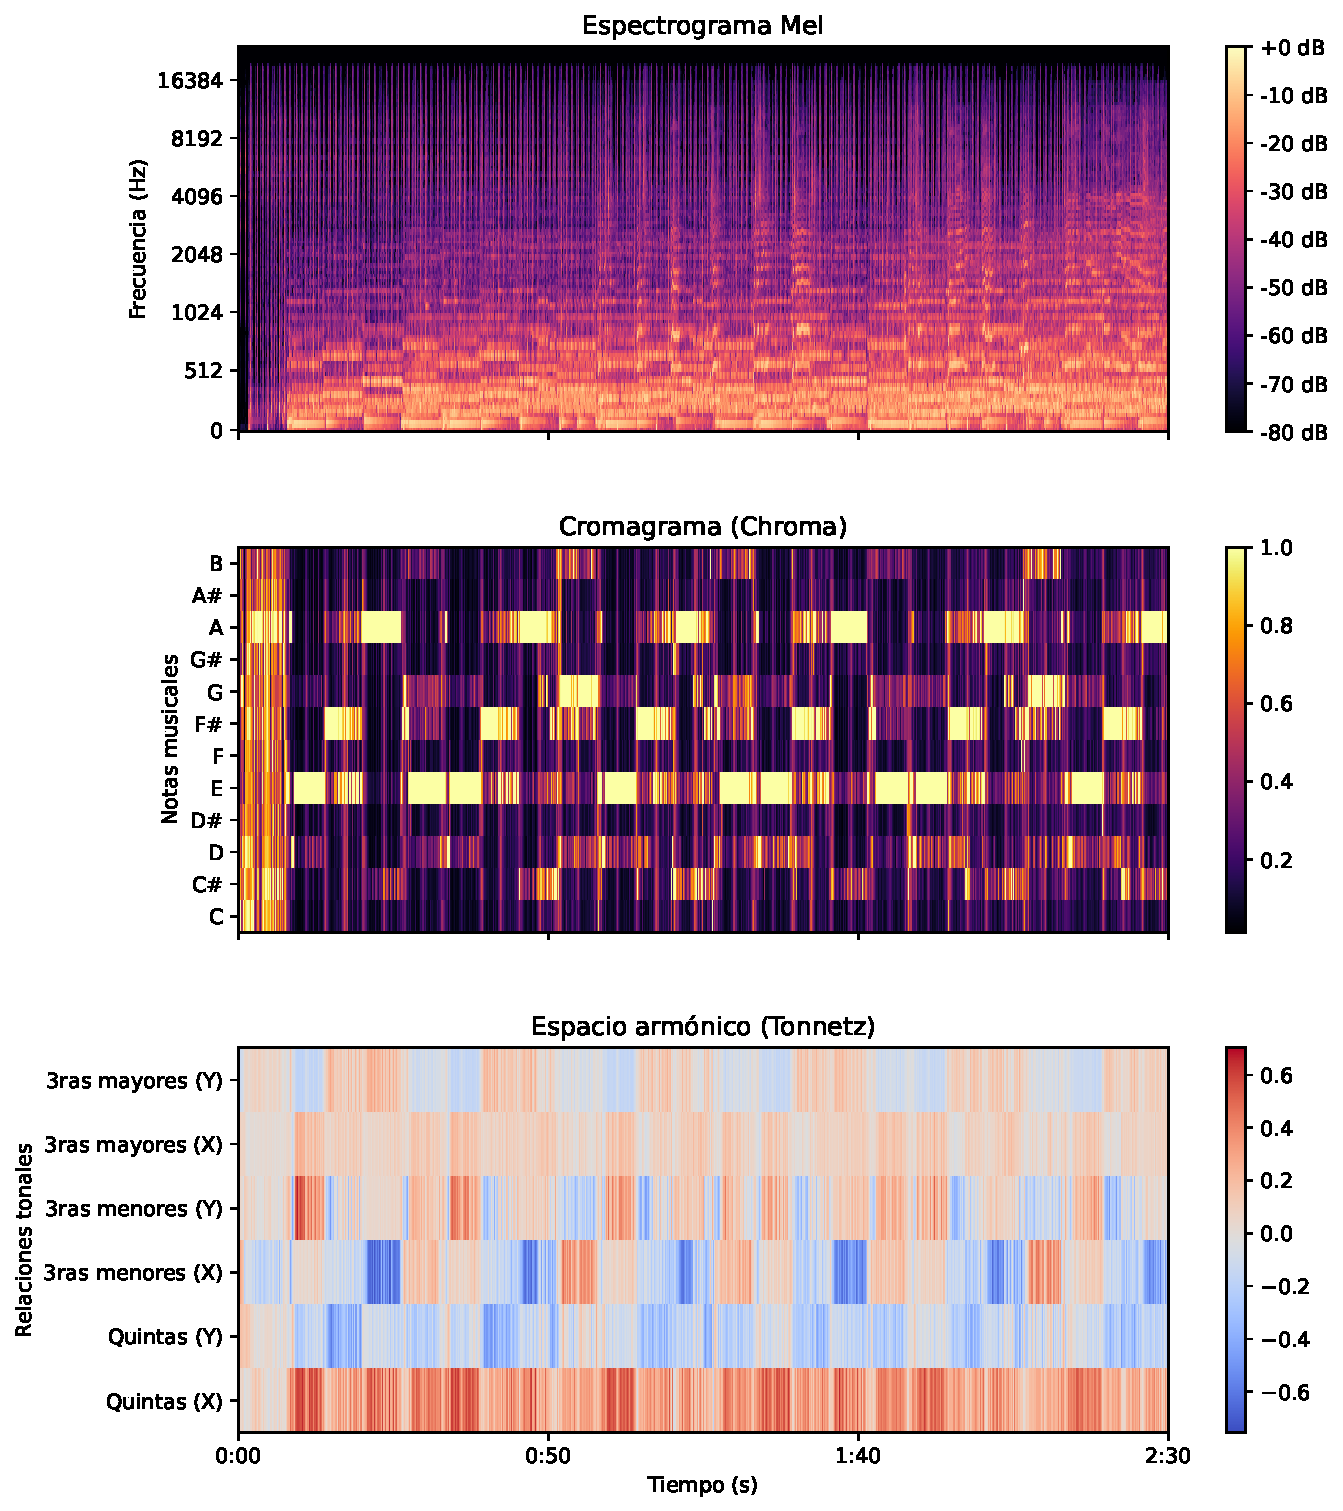
\includegraphics[width=1\textwidth]{./Figures/espectro_croma_tonnetz.pdf}
    \caption[Representaciones visuales del audio]{Representación visual de un espectrograma, un cromagrama y un tonnetz.}
    \label{fig:representaciones_2d}
\end{figure}

Además de las representaciones bidimensionales, las bibliotecas de procesamiento de señales facilitan la extracción de atributos numéricos unidimensionales. En la tabla \ref{tab:atributos_dsp} se presenta un listado que introduce algunas de las características de bajo nivel más representativas en el análisis musical. En la elaboración del trabajo se usaron Librosa y Essentia en este proceso.

Estas transformaciones matemáticas reducen la dimensionalidad del archivo de audio. Sin embargo, carecen de significado semántico. Su función principal, en el contexto de este trabajo, es la de generar las variables predictivas necesarias para entrenar modelos de aprendizaje automático.

El listado completo de las variables de entrada, el análisis de su relevancia y su impacto en el rendimiento de los algoritmos se detalla en el Capítulo 3.

\begin{table}[htpb]
    \centering
    \caption[Atributos representativos]{Listado introductorio de los principales atributos de procesamiento de señales extraídos del audio.}
    \renewcommand{\arraystretch}{1.2}
    \begin{tabular}{p{3.5cm} p{8.5cm}}    
        \toprule
        \textbf{Atributo} & \textbf{Descripción principal} \\
        \midrule
        MFCC & Coeficientes cepstrales que modelan la percepción auditiva humana. \\       
        Centroide espectral & Indica el centro de masa del espectro acústico. Se asocia al brillo del sonido. \\
        Ancho de banda & Mide la dispersión de las frecuencias alrededor del centroide espectral. \\
        Tasa de cruces por cero & Cuantifica la cantidad de cambios de signo en la señal temporal. \\
        Rolloff espectral & Estima la frecuencia por debajo de la que se concentra la mayor parte de la energía. \\
        \bottomrule
    \end{tabular}
    \label{tab:atributos_dsp}
\end{table}

\section{Información semántica del audio}
\label{sec:semantica}

Las representaciones de bajo nivel descritas en la sección 2.2 no siempre son suficientes para capturar conceptos musicales complejos. Es posible mejorar la cobertura de la información musical con el aprendizaje por transferencia. Esta técnica consiste en utilizar modelos previamente entrenados con grandes volúmenes de datos para extraer características semánticas de alto nivel.

Para este fin existen bibliotecas especializadas, como PANNs Inference. Esta herramienta provee acceso a redes neuronales optimizadas para el análisis de eventos sonoros. Dentro de sus opciones, destaca la arquitectura denominada CNN14 \citep{kong2020panns}. Se trata de una red neuronal convolucional, capaz de abstraer patrones del audio y generar embeddings numéricos basados en las clases del conjunto de datos AudioSet. 

Un ejemplo de las probabilidades de detección obtenidas para distintas clases de eventos sonoros a lo largo del tiempo se visualiza en la figura \ref{fig:mapa_semantico}, donde se muestran ventanas consecutivas de 10 segundos de la canción de Radiohead. En este mapa de calor, las áreas más claras indican una mayor probabilidad de activación para cada clase.

El uso de esta arquitectura permite transformar la onda sonora para extraer embeddings y obtener probabilidades asociadas a etiquetas predefinidas, como la presencia de aplausos, instrumentos musicales específicos o habla. Estos datos semánticos enriquecen el conjunto de variables de entrada para la inferencia de algunas de las características musicales que se definieron en el alcance del trabajo.

\newpage
\begin{figure}[!htpb]
    \centering
    
\includegraphics[width=1\textwidth]{mapa_top_clases.pdf}
    \caption[Probabilidades de detección semántica]{Mapa de calor de las características semánticas extraídas mediante la red CNN14.}
    \label{fig:mapa_semantico}
\end{figure}

\section{Modelos de inteligencia artificial utilizados}
\label{sec:modelos}

Una vez obtenidos los descriptores numéricos y semánticos, es necesario aplicar algoritmos de predicción. Para este fin, se utilizaron dos enfoques principales:

\begin{itemize}
    \item Algoritmos LightGBM: se integró la arquitectura LightGBM, basada en el ensamble de árboles de decisión. Esta herramienta destaca por su alta velocidad computacional y eficiencia en tareas generales de predicción.
    \item Redes MLP: los perceptrones multicapa son redes neuronales artificiales con capacidad para modelar relaciones complejas. Permiten, entre otras aplicaciones, predecir múltiples variables continuas de forma simultánea.
\end{itemize}

\section{Despliegue e integración}
\label{sec:despliegue}

La integración del sistema predictivo requirió del despliegue de una interfaz de programación de aplicaciones. Para su construcción se utilizó FastAPI \citep{ramirez2018fastapi} como marco de trabajo. Esta herramienta facilita el desarrollo de servicios web de alto rendimiento basados en Python \citep{python3}.

El alojamiento remoto del producto se apoyó en los servicios de infraestructura de OCI (por su sigla en inglés, Oracle Cloud Infrastructure) \citep{oracle_oci}. Se provisionó una instancia de cómputo virtual en la nube para desplegar la aplicación y ejecutar los modelos predictivos. El uso de esta tecnología garantiza la disponibilidad continua del sistema.

%     \centering
%     \includegraphics[width=0.9\textwidth]{./Figures/diagrama_bloques.pdf}
%     \caption{Diagrama de bloques del sistema en su entorno de despliegue en la nube.}
%     \label{fig:diagrama_despliegue}
% \end{figure}


% \subsection{Uso de mayúscula inicial para los título de secciones}

% Si en el texto se hace alusión a diferentes partes del trabajo referirse a ellas como capítulo, sección o subsección según corresponda. Por ejemplo: ``En el capítulo \ref{Chapter1} se explica tal cosa'', o ``En la sección \ref{sec:ejemplo} se presenta lo que sea'', o ``En la subsección \ref{subsec:ejemplo} se discute otra cosa''.

% Cuando se quiere poner una lista tabulada, se hace así:

% \begin{itemize}
% 	\item Este es el primer elemento de la lista.
% 	\item Este es el segundo elemento de la lista.
% \end{itemize}

% Notar el uso de las mayúsculas y el punto al final de cada elemento.

% Si se desea poner una lista numerada el formato es este:

% \begin{enumerate}
% 	\item Este es el primer elemento de la lista.
% 	\item Este es el segundo elemento de la lista.
% \end{enumerate}

% Notar el uso de las mayúsculas y el punto al final de cada elemento.

% \subsection{Este es el título de una subsección}
% \label{subsec:ejemplo}

% Se recomienda no utilizar \textbf{texto en negritas} en ningún párrafo, ni tampoco texto \underline{subrayado}. En cambio sí se debe utilizar \textit{texto en itálicas} para palabras en un idioma extranjero, al menos la primera vez que aparecen en el texto. En el caso de palabras que estamos inventando se deben utilizar ``comillas'', así como también para citas textuales. Por ejemplo, un \textit{digital filter} es una especie de ``selector'' que permite separar ciertos componentes armónicos en particular.

% La escritura debe ser impersonal. Por ejemplo, no utilizar ``el diseño del firmware lo hice de acuerdo con tal principio'', sino ``el firmware fue diseñado utilizando tal principio''. 

% El trabajo es algo que al momento de escribir la memoria se supone que ya está concluido, entonces todo lo que se refiera a hacer el trabajo se narra en tiempo pasado, porque es algo que ya ocurrió. Por ejemplo, "se diseñó el firmware empleando la técnica de test driven development".

% En cambio, la memoria es algo que está vivo cada vez que el lector la lee. Por eso transcurre siempre en tiempo presente, como por ejemplo:

% ``En el presente capítulo se da una visión global sobre las distintas pruebas realizadas y los resultados obtenidos. Se explica el modo en que fueron llevados a cabo los test unitarios y las pruebas del sistema''.

% Se recomienda no utilizar una sección de glosario sino colocar la descripción de las abreviaturas como parte del mismo cuerpo del texto. Por ejemplo, RTOS (\textit{Real Time Operating System}, Sistema Operativo de Tiempo Real) o en caso de considerarlo apropiado mediante notas a pie de página.

% Si se desea indicar alguna página web utilizar el siguiente formato de referencias bibliográficas, dónde las referencias se detallan en la sección de bibliografía de la memoria, utilizado el formato establecido por IEEE en \citep{IEEE:citation}. Por ejemplo, ``el presente trabajo se basa en la plataforma EDU-CIAA-NXP \citep{CIAA}, la cual...''.

% \subsection{Figuras} 

% Al insertar figuras en la memoria se deben considerar determinadas pautas. Para empezar, usar siempre tipografía claramente legible. Luego, tener claro que \textbf{es incorrecto} escribir por ejemplo esto: ``El diseño elegido es un cuadrado, como se ve en la siguiente figura:''

% \begin{figure}[h]
% \centering
% \includegraphics[scale=.45]{./Figures/cuadradoAzul.png}
% \end{figure}

% La forma correcta de utilizar una figura es con referencias cruzadas, por ejemplo: ``Se eligió utilizar un cuadrado azul para el logo, como puede observarse en la figura \ref{fig:cuadradoAzul}''.

% \begin{figure}[ht]
% 	\centering
% 	\includegraphics[scale=.45]{./Figures/cuadradoAzul.png}
% 	\caption{Ilustración del cuadrado azul que se eligió para el diseño del logo.}
% 	\label{fig:cuadradoAzul}
% \end{figure}

% El texto de las figuras debe estar siempre en español, excepto que se decida reproducir una figura original tomada de alguna referencia. En ese caso la referencia de la cual se tomó la figura debe ser indicada en el epígrafe de la figura e incluida como una nota al pie, como se ilustra en la figura \ref{fig:palabraIngles}.

% \begin{figure}[htpb]
% 	\centering
% 	\includegraphics[scale=.3]{./Figures/word.jpeg}
% 	\caption{Imagen tomada de la página oficial del procesador\protect\footnotemark.}
% 	\label{fig:palabraIngles}
% \end{figure}

% \footnotetext{Imagen tomada de \url{https://goo.gl/images/i7C70w}}

% La figura y el epígrafe deben conformar una unidad cuyo significado principal pueda ser comprendido por el lector sin necesidad de leer el cuerpo central de la memoria. Para eso es necesario que el epígrafe sea todo lo detallado que corresponda y si en la figura se utilizan abreviaturas entonces aclarar su significado en el epígrafe o en la misma figura.



% \begin{figure}[ht]
% 	\centering
% 	\includegraphics[scale=.37]{./Figures/questionMark.png}
% 	\caption{¿Por qué de pronto aparece esta figura?}
% 	\label{fig:questionMark}
% \end{figure}

% Nunca colocar una figura en el documento antes de hacer la primera referencia a ella, como se ilustra con la figura \ref{fig:questionMark}, porque sino el lector no comprenderá por qué de pronto aparece la figura en el documento, lo que distraerá su atención.

% Otra posibilidad es utilizar el entorno \textit{subfigure} para incluir más de una figura, como se puede ver en la figura \ref{fig:three graphs}. Notar que se pueden referenciar también las figuras internas individualmente de esta manera: \ref{fig:1de3}, \ref{fig:2de3} y \ref{fig:3de3}.
 
% \begin{figure}[!htpb]
%      \centering
%      \begin{subfigure}[b]{0.3\textwidth}
%          \centering
%          \includegraphics[width=.65\textwidth]{./Figures/questionMark}
%          \caption{Un caption.}
%          \label{fig:1de3}
%      \end{subfigure}
%      \hfill
%      \begin{subfigure}[b]{0.3\textwidth}
%          \centering
%          \includegraphics[width=.65\textwidth]{./Figures/questionMark}
%          \caption{Otro.}
%          \label{fig:2de3}
%      \end{subfigure}
%      \hfill
%      \begin{subfigure}[b]{0.3\textwidth}
%          \centering
%          \includegraphics[width=.65\textwidth]{./Figures/questionMark}
%          \caption{Y otro más.}
%          \label{fig:3de3}
%      \end{subfigure}
%         \caption{Tres gráficos simples.}
%         \label{fig:three graphs}
% \end{figure}

% El código para generar las imágenes se encuentra disponible para su reutilización en el archivo \file{Chapter2.tex}.

% \subsection{Tablas}

% Para las tablas utilizar el mismo formato que para las figuras, sólo que el epígrafe se debe colocar arriba de la tabla, como se ilustra en la tabla \ref{tab:peces}. Observar que sólo algunas filas van con líneas visibles y notar el uso de las negritas para los encabezados.  La referencia se logra utilizando el comando \verb|\ref{<label>}| donde label debe estar definida dentro del entorno de la tabla.

% \begin{verbatim}
% \begin{table}[h]
% 	\centering
% 	\caption[caption corto]{caption largo más descriptivo}
% 	\begin{tabular}{l c c}    
% 		\toprule
% 		\textbf{Especie}     & \textbf{Tamaño} & \textbf{Valor}\\
% 		\midrule
% 		Amphiprion Ocellaris & 10 cm           & \$ 6.000 \\		
% 		Hepatus Blue Tang    & 15 cm           & \$ 7.000 \\
% 		Zebrasoma Xanthurus  & 12 cm           & \$ 6.800 \\
% 		\bottomrule
% 		\hline
% 	\end{tabular}
% 	\label{tab:peces}
% \end{table}
% \end{verbatim}


% \begin{table}[h]
% 	\centering
% 	\caption[caption corto]{caption largo más descriptivo.}
% 	\begin{tabular}{l c c}    
% 		\toprule
% 		\textbf{Especie} 	 & \textbf{Tamaño} 		& \textbf{Valor}  \\
% 		\midrule
% 		Amphiprion Ocellaris & 10 cm 				& \$ 6.000 \\		
% 		Hepatus Blue Tang	 & 15 cm				& \$ 7.000 \\
% 		Zebrasoma Xanthurus	 & 12 cm				& \$ 6.800 \\
% 		\bottomrule
% 		\hline
% 	\end{tabular}
% 	\label{tab:peces}
% \end{table}

% En cada capítulo se debe reiniciar el número de conteo de las figuras y las tablas, por ejemplo, figura 2.1 o tabla 2.1, pero no se debe reiniciar el conteo en cada sección. Por suerte la plantilla se encarga de esto por nosotros.

% \subsection{Ecuaciones}
% \label{sec:Ecuaciones}

% Al insertar ecuaciones en la memoria dentro de un entorno \textit{equation}, éstas se numeran en forma automática  y se pueden referir al igual que como se hace con las figuras y tablas, por ejemplo ver la ecuación \ref{eq:metric}.

% \begin{equation}
% 	\label{eq:metric}
% 	ds^2 = c^2 dt^2 \left( \frac{d\sigma^2}{1-k\sigma^2} + \sigma^2\left[ d\theta^2 + \sin^2\theta d\phi^2 \right] \right)
% \end{equation}
                                                        
% Para generar la ecuación \ref{eq:metric} se utilizó el siguiente código:

% \begin{verbatim}
% \begin{equation}
% 	\label{eq:metric}
% 	ds^2 = c^2 dt^2 \left( \frac{d\sigma^2}{1-k\sigma^2} + 
% 	\sigma^2\left[ d\theta^2 + 
% 	\sin^2\theta d\phi^2 \right] \right)
% \end{equation}
% \end{verbatim}

\chapter{Diseño e implementación} % Main chapter title

\label{Chapter3} % Change X to a consecutive number; for referencing this chapter elsewhere, use \ref{ChapterX}

% Todos los capítulos deben comenzar con un breve párrafo introductorio que indique cuál es el contenido que se encontrará al leerlo.  La redacción sobre el contenido de la memoria debe hacerse en presente y todo lo referido al proyecto en pasado, siempre de modo impersonal.

\definecolor{mygreen}{rgb}{0,0.6,0}
\definecolor{mygray}{rgb}{0.5,0.5,0.5}
\definecolor{mymauve}{rgb}{0.58,0,0.82}

%%%%%%%%%%%%%%%%%%%%%%%%%%%%%%%%%%%%%%%%%%%%%%%%%%%%%%%%%%%%%%%%%%%%%%%%%%%%%
% parámetros para configurar el formato del código en los entornos lstlisting
%%%%%%%%%%%%%%%%%%%%%%%%%%%%%%%%%%%%%%%%%%%%%%%%%%%%%%%%%%%%%%%%%%%%%%%%%%%%%
\lstset{ %
  backgroundcolor=\color{white},   % choose the background color; you must add \usepackage{color} or \usepackage{xcolor}
  basicstyle=\footnotesize,        % the size of the fonts that are used for the code
  breakatwhitespace=false,         % sets if automatic breaks should only happen at whitespace
  breaklines=true,                 % sets automatic line breaking
  captionpos=b,                    % sets the caption-position to bottom
  commentstyle=\color{mygreen},    % comment style
  deletekeywords={...},            % if you want to delete keywords from the given language
  %escapeinside={\%*}{*)},          % if you want to add LaTeX within your code
  %extendedchars=true,              % lets you use non-ASCII characters; for 8-bits encodings only, does not work with UTF-8
  %frame=single,	                % adds a frame around the code
  keepspaces=true,                 % keeps spaces in text, useful for keeping indentation of code (possibly needs columns=flexible)
  keywordstyle=\color{blue},       % keyword style
  language=Python,                % the language of the code
  %otherkeywords={*,...},           % if you want to add more keywords to the set
  numbers=left,                    % where to put the line-numbers; possible values are (none, left, right)
  numbersep=5pt,                   % how far the line-numbers are from the code
  numberstyle=\tiny\color{mygray}, % the style that is used for the line-numbers
  rulecolor=\color{black},         % if not set, the frame-color may be changed on line-breaks within not-black text (e.g. comments (green here))
  showspaces=false,                % show spaces everywhere adding particular underscores; it overrides 'showstringspaces'
  showstringspaces=false,          % underline spaces within strings only
  showtabs=false,                  % show tabs within strings adding particular underscores
  stepnumber=1,                    % the step between two line-numbers. If it's 1, each line will be numbered
  stringstyle=\color{mymauve},     % string literal style
  tabsize=2,	                   % sets default tabsize to 2 spaces
  title=\lstname,                  % show the filename of files included with \lstinputlisting; also try caption instead of title
  morecomment=[s]{/*}{*/}
}


Este capítulo detalla el diseño y la implementación del sistema predictivo. Se analizan los conjuntos de datos utilizados, la extracción de atributos del audio y el tratamiento de datos según las distribuciones de las variables objetivo. Asimismo, se describen las técnicas de reducción y selección de variables, el proceso de optimización de los modelos y los resultados de la iteración productiva. Finalmente, se presenta la arquitectura desarrollada para el despliegue y la integración del sistema en un entorno operativo.

%----------------------------------------------------------------------------------------
%	SECTION 1
%----------------------------------------------------------------------------------------
\section{Conjuntos de datos}
\label{sec:conjuntos_datos}
% Aquí se describirá la extracción de datos del audio.

\subsection{Análisis de conjuntos de datos públicos}

La definición de la estrategia para la extracción de atributos se fundamenta en una revisión de conjuntos de datos públicos estandarizados en el ámbito MIR. 
El objetivo fue entender cómo repositorios de referencia, como FMA y Million Song Dataset, representan y estructuran los datos musicales, para decidir su viabilidad en el contexto de aplicación de este trabajo. 

\subsubsection{GTZAN}
Este conjunto de datos se considera el equivalente al MNIST \cite{lecun1998gradient} para el análisis de audio \cite{sturm2014state}, dada su adopción histórica como estándar de evaluación en tareas de clasificación de géneros musicales.
\begin{itemize}
    \item Variables predictivas principales: tempo, representaciones chroma, amplitud media cuadrática (RMS), descriptores espectrales y coeficientes MFCC.
    \item Estructura: 1~000 archivos de audio en crudo limitados a 30 segundos, acompañados de metadatos tabulares e imágenes de espectrogramas de Mel en su versión distribuida mediante Kaggle \citep{gtzan_kaggle}. 
    Todas estas representaciones fueron extraídas utilizando la biblioteca Librosa. Las tablas contienen los atributos calculados sobre la pista completa y también sobre divisiones de 3 segundos para incrementar el volumen de datos de entrenamiento. En ambos escenarios se aplica una reducción de dimensionalidad temporal: las variables se calculan inicialmente sobre micro-ventanas de milisegundos y luego se colapsan a valores estáticos mediante estadísticos de agregación, como la media y la varianza.
    \item Variables objetivo principales en Plusyc: se podría relacionar con \textit{suggested genres}. 
    \item Desventajas: provee segmentos cortos de audio, lo que limita la representatividad de la información musical a nivel de canción; y solo abarca 10 géneros musicales, mientras que Plusyc trabaja con más de 500.
\end{itemize}

\subsubsection{FMA estándar}
Se analiza la versión estándar de FMA, diseñada para superar las limitaciones de tamaño y acceso a las colecciones completa y mediana.
\begin{itemize}
    \item Variables predictivas principales: representaciones chroma, Transformada de Q Constante (CQT), tonnetz, MFCC, RMS, descriptores espectrales y tasa de cruces por cero (ZCR).
    \item Estructura: ofrece recortes de audio de 30 segundos para sus subconjuntos estándar, acompañados de matrices de atributos precomputados distribuidos en formato tabular (CSV). Los atributos fueron extraídos utilizando Librosa y posteriormente colapsados mediante estadísticos de agregación, como la media, desviación estándar, asimetría y curtosis, para obtener valores estáticos por pista.
    \item Metadatos contextuales: información tabular adicional que incluye álbum, artista, popularidad, fechas de lanzamiento y ubicación geográfica.
    \item Variables objetivo principales: géneros musicales estructurados en una taxonomía jerárquica de clases y para un subconjunto de aproximadamente 13~000 pistas, proporciona atributos como \textit{danceability, energy, valence, speechiness} y \textit{liveness}.
    \item Desventajas: el análisis está restringido a segmentos de 30 segundos en la versión estándar. Las versiones media y completa exceden las capacidades de procesamiento de la infraestructura actual de la empresa. Además, la incertidumbre sobre las versiones exactas de Librosa utilizadas originalmente dificulta la replicabilidad técnica sobre canciones nuevas. Finalmente, la información etiquetada de 13~000 pistas es mucho menor que la de más de 60~000 de Plusyc.
\end{itemize}

\subsubsection{Million Song Dataset (MSD)}
Desarrollado por la Universidad de Columbia y The Echo Nest \cite{bertin2011million}, este conjunto escaló la investigación de información musical a nivel industrial.
\begin{itemize}
    \item Variables predictivas principales: representaciones de tono (chroma y pitch) y descriptores de timbre, ambos calculados a nivel de segmento.
    \item Estructura: colección de metadatos y descriptores precomputados empaquetados en archivos HDF5.
    \item Método de extracción: a diferencia de la segmentación por ventanas fijas, el MSD utiliza una división adaptativa basada en eventos. Esto fragmenta la canción en segmentos de duración variable. Para cada uno de estos segmentos, se calculan coeficientes de tono y timbre, y se genera una matriz de atributos alineada con la estructura temporal de la pista.
    \item Variables objetivo principales: proporciona atributos musicales fundamentales como \textit{tempo, loudness, key} y \textit{mode}.
    \item Desventajas: los descriptores se generaron con algoritmos propietarios de The Echo Nest, lo que complica procesar la segmentación por eventos en canciones nuevas de forma idéntica para realizar el proceso de inferencia.
\end{itemize}

\subsubsection{AudioSet}
Este conjunto masivo establece un estándar para la clasificación de eventos sonoros generales
\begin{itemize}
    \item Estructura: conjunto de identificadores de videos de YouTube y marcas de tiempo que referencian segmentos de 10 segundos, anotados bajo una ontología de 527 clases.
    \item Variables predictivas principales: el corpus original no extrae descriptores tradicionales. Su distribución oficial provee embeddings precomputados mediante el modelo VGGish \cite{hershey2017cnn}, que sirven como entrada rápida para entrenar clasificadores de terceros sin necesidad de descargar el audio original.
    \item Variables objetivo principales: etiquetas multiclase que identifican la presencia de instrumentos musicales, como tipos de voces (habla, canto) y ambientes acústicos.
    \item Desventajas: el enfoque en sonidos generales limita su precisión para los atributos musicales.
\end{itemize}

% En la tabla \ref{tab:variables_datasets} se presentan algunas de las variables predictivas más relevantes de cada conjunto de datos.

Todos estos conjuntos de datos presentan varias limitaciones frente a la solución propuesta: algunos restringen el análisis a segmentos cortos de audio, mientras que otros requieren tamaños de almacenamiento excesivamente pesados o estructuras de datos difíciles de replicar durante el proceso de inferencia y dependientes de las versiones de las bibliotecas de extracción.

Por otro lado, estas restricciones motivaron que el proceso de extracción se ejecute directamente sobre el catálogo privado para eliminar las limitaciones, y su revisión permitió sentar las bases para determinar cuáles son las variables predictivas en la música, cómo se segmentan las canciones, cómo se reduce la dimensionalidad y para hacer los primeros experimentos predictivos de las variables objetivo requeridas.

Cabe mencionar que, a pesar de que en algunas de las fuentes de datos públicas se incluye información del contexto como la región del artista, el año de lanzamiento, el álbum o las letras, en esta solución se trabaja exclusivamente con información musical que se extrae del audio. 

\subsection{Reducción de dimensionalidad mediante estadísticas}

En el ámbito del procesamiento de señales, la información de un archivo de audio se representa como una serie de tiempo multivariada: una secuencia de puntos de datos \cite{muller2015fundamentals}, en este caso, descriptores numéricos y semánticos, indexados y ordenados cronológicamente.

La estrategia adoptada se inspiró en los conjuntos de datos de referencia, donde la señal se divide en ventanas temporales y la información de cada ventana se colapsa en valores estáticos. Esto permite reducir estas secuencias a un vector por cada canción, buscando optimizar el uso de la memoria y los tiempos de procesamiento.
Esta transformación de la señal de secuencias de números a un vector de estadísticos ocurre de la siguiente manera:

\begin{itemize}
    \item Segmentación temporal: se estableció una ventana de análisis de 10 segundos continuos. Esta decisión se fundamenta en la arquitectura de la red neuronal CNN14, entrenada sobre el conjunto de datos AudioSet, cuyos segmentos originales son de 10 segundos.
    \item Extracción de variables predictivas: para cada segmento de 10 segundos de la canción, el algoritmo usa Librosa y Essentia para extraer el conjunto de variables predictivas principales que proveen las fuentes de datos públicos. También se extrae información global de la canción y algunas de las variables predictivas escalares se calculan de forma global y también de forma segmentada y agregada.
    \item Extracción de embeddings y probabilidades: para esos segmentos de 10 segundos, el algoritmo también extrae un vector de embeddings y las probabilidades de activación para 173 clases de eventos musicales provistas por PANNs inference.
    \item Agrupación estadística: dado que una canción estándar produce una cantidad variable de segmentos de 10 segundos, se aplicó una técnica de colapso estadístico a lo largo del eje temporal, diferenciando el tratamiento según el tipo de variable:
    \begin{itemize}
        \item Para las variables predictivas (DSP), se calcularon siete estadísticos por pista: media, desviación estándar, asimetría, curtosis, y los percentiles 10 (cerca del mínimo), 50 (mediana) y 90 (cerca del máximo para evitar ruido).
        \item Para los embeddings y las probabilidades semánticas de las 173 clases seleccionadas de PANNs, se calcularon cuatro medidas: media, valor máximo, desviación estándar y el percentil 90.
    \end{itemize}
\end{itemize}

Este enfoque matemático permite comprimir el volumen masivo de información de una serie de tiempo en un único vector unidimensional por canción.

Algunos experimentos preliminares sirvieron para validar que esta representación permitía capturar la información esencial de la canción de manera eficiente y compacta.
El algoritmo de extracción, es el resultado de múltiples pruebas con distintas configuraciones de variables, estadísticos y métodos de segmentación. Algunos de los experimentos que no resultaron exitosos comprenden:
pruebas con solo variables predictivas sin embeddings, demuestran que no es posible capturar eventos como el público en vivo o el habla en los primeros intentos de inferencia de \textit{liveness} y \textit{speechiness}. Las pruebas con embeddings pero sin variables predictivas en general no proporcionan la información de \textit{key}, \textit{tempo}, \textit{loudness}, \textit{mood} o \textit{genres}.
Pruebas con distintas ventanas resultaron ser ineficientes en el proceso de extracción de más de 60~000 canciones. Pruebas aplicando todos los estadísticos resultaron en un espacio de variables que consume mucho espacio de almacenamiento y con alta correlación.

\subsection{Conformación del espacio de variables masivo}
% Tras validar la superioridad de la arquitectura mixta, se ejecutó el proceso de extracción sobre el catálogo completo. El procesamiento computacional requirió más de una semana de ejecución ininterrumpida para procesar las canciones completas.

% El algoritmo de extracción definitivo combinó las funciones de Librosa y Essentia con la inferencia de la red neuronal CNN14. El resultado fue un conjunto de datos masivo compuesto por más de 9000 variables predictivas independientes por cada registro de audio. Este extenso espacio de características garantiza la disponibilidad de toda la información acústica y semántica posible para la etapa de experimentación. El alto costo computacional de la extracción justifica esta estrategia de recopilación exhaustiva, eliminando la necesidad de reprocesar el audio y trasladando el desafío técnico hacia la selección rigurosa de las variables más relevantes durante la etapa de modelado, proceso que se detalla en la sección \ref{sec:seleccion_variables} %.


\section{Ejecución de tareas sobre el conjunto de datos}
\label{sec:ejecucion_tareas}
% Aquí se detallarán las distribuciones de las variables objetivo, dificultades encontradas y estrategias de muestreo.


\section{Selección de variables de entrada}
\label{sec:seleccion_variables}
% Aquí se describirán las técnicas de selección y reducción para una arquitectura mixta.


\section{Modelado y optimización}
\label{sec:modelado_optimizacion}
% Aquí se abordará el proceso de modelado y la búsqueda de hiperparámetros.


\section{Iteración productiva}
\label{sec:iteracion_productiva}
% Aquí se presentarán los resultados generales de la iteración.


\section{Arquitectura de despliegue e integración}
\label{sec:arquitectura_despliegue}
% Aquí se documentará la arquitectura para el despliegue e integración en un ambiente productivo.

% La idea de esta sección es resaltar los problemas encontrados, los criterios utilizados y la justificación de las decisiones que se hayan tomado.
% Se puede agregar código o pseudocódigo dentro de un entorno lstlisting con el siguiente código:




\begin{verbatim}
\begin{lstlisting}[caption= "un epígrafe descriptivo"]
	las líneas de código irían aquí...
\end{lstlisting}
\end{verbatim}

A modo de ejemplo, se muestra el fragmento de código \ref{cod:vControl}:

\begin{lstlisting}[label=cod:vControl,caption=Pseudocódigo del lazo principal de control.]  % Start your code-block

#define MAX_SENSOR_NUMBER 3
#define MAX_ALARM_NUMBER  6
#define MAX_ACTUATOR_NUMBER 6

uint32_t sensorValue[MAX_SENSOR_NUMBER];		
FunctionalState alarmControl[MAX_ALARM_NUMBER];	//ENABLE or DISABLE
state_t alarmState[MAX_ALARM_NUMBER];						//ON or OFF
state_t actuatorState[MAX_ACTUATOR_NUMBER];			//ON or OFF

void vControl() {

	initGlobalVariables();
	
	period = 500 ms;
		
	while(1) {

		ticks = xTaskGetTickCount();
		
		updateSensors();
		
		updateAlarms();
		
		controlActuators();
		
		vTaskDelayUntil(&ticks, period);
	}
}
\end{lstlisting}




% Chapter Template

% todo en la parte de datasets se me sugirió mover aquí esto...
% Algunos de los experimentos que no resultaron exitosos comprenden:
% pruebas con solo variables predictivas sin embeddings, demuestran que no es posible capturar eventos como el público en vivo o el habla en los primeros intentos de inferencia de \textit{liveness} y \textit{speechiness}. Las pruebas con embeddings pero sin variables predictivas en general no proporcionan la información de \textit{key}, \textit{tempo}, \textit{loudness}, \textit{mood} o \textit{genres}.
% Pruebas con distintas ventanas resultaron ser ineficientes en el proceso de extracción de más de 60~000 canciones. Pruebas aplicando todos los estadísticos resultaron en un espacio de variables que consume mucho espacio de almacenamiento y con alta correlación.

\chapter{Ensayos y resultados} % Main chapter title

\label{Chapter4} % Change X to a consecutive number; for referencing this chapter elsewhere, use \ref{ChapterX}
Todos los capítulos deben comenzar con un breve párrafo introductorio que indique cuál es el contenido que se encontrará al leerlo.  La redacción sobre el contenido de la memoria debe hacerse en presente y todo lo referido al proyecto en pasado, siempre de modo impersonal.

%todo Dada la complejidad de objetivos como los géneros musicales, 197 clases resultantes, se priorizó el análisis de la precisión \textit{Top-K} para capturar la pluralidad semántica de la música
%----------------------------------------------------------------------------------------
%	SECTION 1
%----------------------------------------------------------------------------------------

\section{Pruebas funcionales del hardware}
\label{sec:pruebasHW}

La idea de esta sección es explicar cómo se hicieron los ensayos, qué resultados se obtuvieron y analizarlos.

% Chapter Template

\chapter{Conclusiones} % Main chapter title

Este capítulo presenta un resumen de los logros y las dificultades para llegar al estado actual de la solución y sugiere una serie de siguientes pasos para la evolución del sistema.

\label{Chapter5} % Change X to a consecutive number; for referencing this chapter elsewhere, use \ref{ChapterX}

\section{Conclusiones generales}

En este trabajo se propuso diseñar e implementar un sistema capaz de predecir características musicales a partir de audio de canciones. El objetivo principal fue automatizar
un proceso tradicionalmente manual y laborioso de clasificación musical y reducir la dependencia de servicios de tercecros para evitar costos recurrentes.
El trabajo está en producción, clasifica las canciones que ingresan al sistema, es funcional en el contexto de una empresa en crecimiento. 

En relación a los objetivos específicos, se puede concluir que:

%----------------------------------------------------------------------------------------

%----------------------------------------------------------------------------------------
%	SECTION 1
%----------------------------------------------------------------------------------------

\begin{itemize}
\item Se cumplieron los requerimientos técnicos al lograr la caracterización de las variables solicitadas a partir de los datos de Plusyc.
\item La extracción de variables acústicas DSP sirvió para las predicciones, y la inclusión de embeddings y probabilidades de PANNs fue lo que permitió resolver las variables semánticas complejas. Sin esto último, no se habría completado el trabajo.
\item Se aplicaron acciones para mitigar problemas en los datos. Fue necesario aplicar técnicas de preprocesamiento; se cortó el histórico en una fecha específica para aislar un cambio en la distribución de los datos.
\item Se entrenaron modelos de aprendizaje automático para predecir las características musicales y la evaluación de las métricas de rendimiento dan resultados productivos, acorde al análisis y diseño realizados.
\item La decisión de usar bibliotecas como Librosa y PANNs inference y modelos como redes MLP y ensambles de árboles, permitió no depender de licencias ni pagar costos por consultas a modelos de terceros, también facilitó el trabajo al no requerir de arquitecturas complejas.
\item En específico, la clasificación de estados de ánimo y géneros sugiere que la ambigüedad humana al etiquetar afecta el aprendizaje. Estos resultados indican que el equipo de curaduría necesita estandarizar los criterios para la ingesta manual de datos.
\item Para la detección de público en vivo y habla en canciones, se requirió de limpieza de ruido por falsas etiquetas apoyada en un modelo preentrenado con el conjunto de datos AudioSet, creado para la generación automática de subtítulos como [Aplausos] o [Rapping].
\item Completar el trabajo tomó más tiempo del planificado en el cronograma original. Hubo una subestimación del esfuerzo, dado que la cantidad de modelos y el proceso de aprendizaje requirieron más iteraciones de las previstas.

\end{itemize}

\section{Próximos pasos}

Los diseños actuales quedan disponibles y se pueden usar para iteraciones futuras. Algunos aspectos que se podrían mejorar o explorar son:

\begin{itemize}
\item El uso de las inferencias de PANNs y la exploración de otros modelos preentrenados, para mejorar la limpieza de algunos datos y corregir audios mal etiquetados.
Como ejemplos, el \textit{speechiness}, \textit{liveness} y la predicción de \textit{instrumentalness}: el modelo actual logra diferenciar una canción instrumental de una que no lo es, pero los valores en el medio no son claros. 
Se sugiere revisar puntualmente, ya que presenta ruido en los valores intermedios por falta de definiciones claras.
\item También se sugiere iterar sobre el \textit{tempo} para buscar una solución más robusta que el algoritmo de DSP.
\item Se propone empezar a usar el estado de ánimo secundario como filtro en Plusyc para mejorar la precisión de las recomendaciones musicales.
\item El sistema se puede ajustar para el despliegue bajo el modelo de software como servicio y así permitir ofrecer el servicio al público interesado.
\item El equipo de curadores sigue clasificando música. Se contempla automatizar un reentrenamiento periódico para que el sistema aprenda nuevos géneros cada vez que una clase alcance un mínimo de 100 muestras, con el uso de tecnologías como Airflow y MLflow para optimizar estos procesos, hoy manuales.
\item Se podría evaluar a futuro el uso de arquitecturas basadas en transformadores, si se cuenta con mayor capacidad de cómputo, para mejorar la clasificación de clases densas. 
También, complementar el sistema con modelos de aprendizaje profundo enfocados exclusivamente en música.
\end{itemize}
%----------------------------------------------------------------------------------------

%   SECTION 2

%----------------------------------------------------------------------------------------

% \section{Próximos pasos}



% Acá se indica cómo se podría continuar el trabajo más adelante.



% \section{Conclusiones generales}

% % Este capítulo resume los hallazgos del proyecto y establece la hoja de ruta para su evolución en Plusyc.

% \begin{itemize}
% \item Se cumplió la totalidad de los requerimientos técnicos al lograr la caracterización de las variables acústicas solicitadas.
% \item La ejecución tomó más tiempo del planificado en el cronograma original. Hubo una subestimación del esfuerzo, ya que la cantidad de modelos obligó a iterar más de lo previsto para encontrar resultados aceptables.
% \item Se aplicaron acciones para mitigar problemas en los datos. Se cortó el histórico en enero de 2026 para aislar un cambio en la distribución de los registros. Además, se usó submuestreo y limpieza con modelos preentrenados para compensar el desbalance en clases como liveness y speechiness.
% \item La extracción de variables acústicas tradicionales sirvió como base, pero la inclusión de embeddings y probabilidades de PANNs fue lo que permitió resolver las variables semánticas complejas. Sin esto último, no se habría completado el trabajo.
% \item La clasificación de estados de ánimo y géneros demostró que la ambigüedad humana al etiquetar afecta el aprendizaje. Estos resultados indican que el equipo de curaduría necesita estandarizar los criterios para la ingesta manual de datos.
% \item Se optó por usar PyTorch y PANNs para no depender de licencias ni pagar costos por consultas a modelos de terceros. El sistema se desplegó bajo el modelo de software como servicio para facilitar un procesamiento escalable y asíncrono.
% \end{itemize}

% \section{Próximos pasos}

% % Acá se indica cómo se podría continuar el trabajo más adelante.

% \begin{itemize}
% \item Los modelos actuales quedan como base para iteraciones futuras. Se debe revisar puntualmente instrumentalness, ya que presenta mucho ruido por falta de definiciones claras en los valores intermedios.
% \item Se deja como trabajo pendiente usar las inferencias de PANNs para automatizar la limpieza de datos en el histórico y corregir audios mal etiquetados.
% \item El equipo de curadores sigue clasificando música. Se contempla automatizar un reentrenamiento periódico para que el sistema aprenda nuevos géneros cada vez que una clase alcance un mínimo de 100 muestras.
% \item Se propone empezar a usar el estado de ánimo secundario como filtro en Plusyc para mejorar la precisión de las recomendaciones musicales.
% \item Se sugiere evaluar a futuro el uso de arquitecturas basadas en transformadores para audios, si se cuenta con mayor capacidad de cómputo, para buscar mejoras en la clasificación de clases densas como los géneros.
% \end{itemize}

%----------------------------------------------------------------------------------------
% Apéndices
%----------------------------------------------------------------------------------------

\appendix

% Incluir apéndices desde archivos separados si es necesario
%\chapter{Apéndice A: variables predictivas por tipo y modelo}
\label{AppendixA}

Se detalla la cantidad y proporción de los tipos de variable predictiva.

\begin{table}[htpb]
    \centering
    \caption{Distribución del tipo de variables predictivas en los modelos.}
    \label{tab:proporcion_variables}
    \renewcommand{\arraystretch}{1.2}
    % Aquí inicia el ajuste al ancho de la página
    \resizebox{\textwidth}{!}{%
    \begin{tabular}{@{}lccccc@{}}
        \toprule
        \multirow{2}{*}{\textbf{Variable objetivo}} & \multirow{2}{*}{\textbf{Total}} & \multirow{2}{*}{\textbf{DSP}} & \multicolumn{3}{c}{\textbf{PANNs}} \\
        \cmidrule(l){4-6}
        & & & \textbf{Emb.} & \textbf{Prob.} & \textbf{Total (\%)} \\
        \midrule
        \textit{Key} y \textit{mode}        & 173  & 173 (100\,\%) & 0           & 0          & 0 (0,0\,\%) \\
        \textit{Perceptibles (MLP)}         & 2 140 & 480 (22,4\,\%) & 1 315       & 345        & 1 660 (77,6\,\%) \\
        \textit{Speechiness}                & 92   & 22 (23,9\,\%)  & 62          & 8          & 70 (76,1\,\%) \\
        \textit{Liveness}                   & 76   & 24 (31,6\,\%)  & 36          & 16         & 52 (68,4\,\%) \\
        \textit{Primary mood}               & 1 423 & 382 (26,8\,\%) & 1 010       & 31         & 1 041 (73,2\,\%) \\
        \textit{Secondary mood}             & 1 397 & 385 (27,6\,\%) & 980         & 32         & 1 012 (72,4\,\%) \\
        \textit{Suggested genres}           & 1 309 & 370 (28,3\,\%) & 912         & 27         & 939 (71,7\,\%) \\
        \bottomrule
    \end{tabular}%
    } % Aquí cierra el resizebox
\end{table}

%----------------------------------------------------------------------------------------
% Bibliografía
%----------------------------------------------------------------------------------------

\renewcommand{\bibname}{Bibliografía} % Para asegurarte de que el título sea correcto
\phantomsection % Necesario para que el enlace del marcador sea correcto

\printbibliography[heading=bibintoc]

\end{document}






